\documentclass{beamer}
%
% Choose how your presentation looks.
%
% For more themes, color themes and font themes, see:
% http://deic.uab.es/~iblanes/beamer_gallery/index_by_theme.html
%
\mode<presentation>
{
  \usetheme{Madrid}      % or try Darmstadt, Madrid, Warsaw, ...
  \usecolortheme{beaver} % or try albatross, beaver, crane, ...
  \usefonttheme{serif}  % or try serif, structurebold, ...
  \setbeamertemplate{navigation symbols}{}
  \setbeamertemplate{caption}[numbered]
} 


\usepackage[utf8]{inputenc}
% \usepackage[latin1]{inputenc}
\usepackage[T1]{fontenc}
\usepackage[portuges,brazilian]{babel}
\usepackage{graphicx,hyperref,url}
\usepackage{lmodern}
\usepackage{caption}
\usepackage{subfigure}
%\usepackage{subcaption}
\usepackage{latexsym}
\usepackage{amssymb, amsmath}
\usepackage{multicol}
\usepackage{pifont} 
%%%,bbding}%%,dingbat} %%% ver manual de simbolos
\usepackage{listings}
\usepackage{comment}
\usepackage{sansmathaccent}
\usepackage{qtree}
%\pdfmapfile{+sansmathaccent.map}
\usepackage{wasysym} %% tem carinhas

\definecolor{azulclaro}{rgb}{0.9,0.9,0.9}
\definecolor{mygreen}{rgb}{0,0.6,0}
\definecolor{mygray}{rgb}{0.5,0.5,0.5}
\definecolor{mymauve}{rgb}{0.58,0,0.82}
\definecolor{darkgray}{rgb}{.4,.4,.4}
\definecolor{purple}{rgb}{0.65, 0.12, 0.82}

%\newcommand{\minizinc}{MiniZinc}

% (TODO) review
 \lstset{ 
 %  label={pgm_ex01},
     backgroundcolor=\color{azulclaro}, 
     language=C, %%Miranda,%%Perl,%%%Python, %%Mercury,
     showstringspaces=false,
     basicstyle=\bf\scriptsize\ttfamily,
% %%      basicstyle= \footnotesize %%% TESTAR
      keywordstyle=\bfseries\color{green!40!black},
%     keywordstyle=\textbf{\color{mygreen}}, 
%     otherkeywords={*, \%, array, constraint, solve, output,  show, "/\", satisfy, set, of, if, then, elseif, float, search},
% %%  keywordstyle=\color{blue},       % keyword style
% %%    commentstyle=\itshape\color{purple!40!black},
       commentstyle=\color{orange},    % comment style
       identifierstyle=\color{blue},
       stringstyle=\color{orange},
%       stringstyle=\color{mymauve},
       numbers=left,  % where to put the line-numbers; possible values are (none, left, right)
       numbersep=5pt,   % how far the line-numbers are from the code
       numberstyle=\tiny\color{magenta},
       keepspaces=true      
%     % %caption={LEGENDA no source PASCAL ficou OK},
 }
 
\graphicspath
{ 
	% {/home/ccs/Dropbox/figs_genericas/}%
	% {figuras/}%
	% {/home/ccs/Dropbox/CCS/picat/}%
	{figs/fig_ponteiros/}%
	{figs/fig_recursao/}%
	{figs/fig_arvores/}%
	{figs/fig_filas/}%
	{figs/fig_hash/}%
	{figs/fig_listas/}%
	{figs/fig_pilhas/}%
}
 
\DeclareGraphicsExtensions{.pdf,.png,.jpg,.jpeg}

%Global Background must be put in preamble
%\usebackgroundtemplate{\includegraphics[width=\paperwidth]{amarelinho.pdf}}
%%% \begin{frame}[allowframebreaks=0.8]

% The log drawn in the upper right corner.

%\logo{\centering
%\includegraphics[height=0.050\paperheight]{figuras/logo_SBPO_Peixe.png}
%%\hspace{9.6cm}
%\includegraphics[height=0.027\paperheight]{figuras/logo_udesc_horizontal.jpg}


%%%%%%%%%%%%%%%%%%%%%%%%%%%%%%%%%%%%%%%%%%%%%%%%%%%%%%%%%%%%%%%%%%%%%

\title[EDA]{\fontsize{20}{30}\selectfont \textcolor{black}{Estrutura de Dados}}

\author[]{Claudio Cesar de Sá, Alessandro Ferreira Leite,
Lucas Hermman Negri, Gilmário Barbosa}
%\\     {\small \url{claudio.sa@udesc.br}}

\institute[UDESC]{
    Departamento de Ci\^encia da Computa\c{c}\~ao \\
    Centro de Ci\^encias e Tecnol\'ogias\\
   Universidade do Estado de Santa Catarina}

\date{\today}

\AtBeginSection[]
{
  \begin{frame}<beamer>
    \frametitle{Onde estamos ...}
    \tableofcontents[currentsection,currentsubsection]
  \end{frame}
}
%%%%%%%%%%%%%%%%%%%%%%%%%%%%%%%%%%%%%%%%%%%%%%%%%%%%%%%%%%%%%%%%%%%%%

\begin{document}

\begin{frame}
    \titlepage
\end{frame}

%%%%%%%%%%%%%%%%%%%%%%%%%%%%%%%%%%%%%%%%%%%%%%%%%%%%%%%%%%%%%%%%%%%%%

\begin{frame} [allowframebreaks=0.7]
\frametitle{Sumário}
\tableofcontents
\end{frame}

%%%%%%%%%%%%%%%%%%%%%%%%%%%%%%%%%%%%%%%%%%%%%%%%%%%%%%%%%%%%%%%%%%%%%

\begin{frame}[fragile]
\frametitle{Agradecimentos}

Vários autores e colaboradores ...
\begin{itemize}
 % \item Alessandro Ferreira Leite --
 % \item Lucas Hermman Negri -- IFMS
 % \item Gilmário Barbosa -- UDESC
 \item Ao Google Images ... 
  
\end{itemize}

\end{frame}



%%%%%%%%%%%%%%%%%%%%%%%%%%%%%%%%%%%%%%%%%%%%%%%%%%%%%%%%%%%%%%%%%%%%%
%!TEX root = curso_EDA_SLIDES.tex

\section{O Curso}
\begin{frame}


\frametitle{Disciplina}

\begin{block}{Estrutura de Dados -- EDA001}

\begin{itemize}
\item \emph{\textbf{Turma:}} 
\item \emph{\textbf{Professor:}} Claudio Cesar de Sá
  \begin{itemize}
  \item \texttt{claudio.sa@udesc.br}
  \item Sala 13 Bloco F
  \end{itemize}
\item \emph{\textbf{Carga horária:}} 72 horas-aula 
\textcolor{red}{$\bullet$}~Teóricas: 36 \textcolor{red}{$\bullet$}~Práticas: 36
\item \emph{\textbf{Curso:}} BCC
\item \emph{\textbf{Requisitos:}} LPG, Linux, sólidos conhecimentos da linguagem C -- há um documento específico sobre isto
%\item \emph{\textbf{Período:}} 2º semestre de 2017
\item \emph{\textbf{Período:}} 1º semestre de 2018
\item \emph{\textbf{Horários:}}
  \begin{itemize}
  \item 3ª 15h20 (2 aulas) - F-205  -- aula expositiva
  \item 5ª 15h20 (2 aulas) - F-205 -- lab
  
  \end{itemize}

\end{itemize}

\end{block}

\end{frame}


%-------------------------------------
\begin{frame}
\frametitle{Ementa}

\begin{block}{Ementa}
Representação e manipulação de tipos abstratos de dados. Estruturas lineares. 
Introdução a estruturas hierárquicas. Métodos de classificação. Análise de eficiência. Aplicações.
\end{block}

\end{frame}

%-------------------------------------
\begin{frame} [allowframebreaks=0.9]
\frametitle{Objetivos}

\begin{itemize}
\item \emph{\textbf{Geral:}} 
 
 \textcolor{red}{Há um documento específico sobre isto $=$ Plano de Ensino}


\newpage
\item \emph{\textbf{Específicos:}} 

    \textcolor{red}{Há um documento específico sobre isto $=$ Plano de Ensino}


\end{itemize}

\end{frame}

%-----------------------------------------------------------------------

\begin{frame}
\frametitle{Livros que estarei usando ...}

\begin{columns}
\begin{column}{.5\textwidth}
\centering
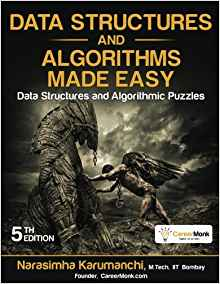
\includegraphics[height=6cm, width=5cm]{figs/fig_gerais/capa_livro_made_easy.jpeg}

\end{column}

\begin{column}{.5\textwidth}
\centering

\includegraphics[height=6cm, width=5cm]{figs/fig_gerais/capa_livro_program_design_C.jpeg}

\end{column}

\end{columns}


\end{frame}
%-----------------------------------------------------------------------

\begin{frame}
\frametitle{Conteúdo programático}

   \textcolor{red}{Há um documento específico sobre isto $=$ Plano de Ensino}
    
\end{frame}


%-----------------------------------------------------------------------
\begin{frame}
\frametitle{Bibliografia UDESC}

    \textcolor{red}{Há um documento específico sobre isto $=$ Plano de Ensino}
      
 \end{frame}

%-----------------------------------------------

\begin{frame}
\frametitle{Conteúdo programático}

 \textcolor{red}{Há um documento específico sobre isto $=$ Plano de Ensino}

\end{frame}
---------------------------

\subsection{Ferramentas}
\begin{frame}

    \frametitle{Ferramentas ... nesta ordem}

  \begin{itemize}
   \item Linux (veja o diret\'orio de linux no GitHub deste curso)
   \item Algumas aulas sobre uso comandos do Linux (nivelamento)
    \item Linguagem C (ora o compilador g++)
    \item Codeblock, Geany, Sublime, Atom, etc
            

      % \url{http://ccl.northwestern.edu/netlogo/docs/} (escondido in WEB)
      
    \end{itemize}
\end{frame}

%%%%%%%%%%%%%%%%%%%%%%%%%%%%%%%%%%%%%%%%%%%%%%%%%%%%%%%%%%%%%%%%%%%%%

\subsection{Metodologia e avaliação}  

\begin{frame}[allowframebreaks=0.9]

\frametitle{Metodologia e avaliação}

\textbf{Metodologia:} \\

\textit{As aulas serão expositivas e práticas. A cada novo assunto tratado, exemplos  são demonstrados utilizando ferramentas computacionais adequadas
  para consolidar os conceitos 
 tratados.
 }
 \pause
 $\Rightarrow  $ Na sequ\^encia avaliaç\~oes .... a cada 15 a 21 dias!

\newpage
    \textbf{Avaliação}

    \begin{itemize}
    \item n-provas -- $\approx$  90\%\\
      
	\quad \textcolor{red}{$\bullet$}~$P_1$: xx/mar ou ago\\
	\quad \textcolor{red}{$\bullet$}~$P_2$: xx/abril ou set\\
		\quad \textcolor{red}{$\bullet$}~$P_3$: xx/maio ou set\\
	\quad \textcolor{red}{$\bullet$}~$P_4$: xx/junho ou out\\
		\quad \textcolor{red}{$\bullet$}~$P_5$: xx/junho ou nov\\
		\quad \textcolor{red}{$\bullet$}~$TF$: Trabalho Final sobre \'arvores $\approx$  10\%\\
	\quad \textcolor{red}{$\bullet$}~$P_F$: 2x/junho ou nov\\(provão: todo conteúdo)

      \item Exercícios de laboratório  -- $\approx $ pouco ... \%
             
      \item Presença e participação: 75\% é o mínimo obrigatório
      para a UDESC. Quem quiser faltar por razões diversas,
       ou assuntos específicos, trate pessoalmente com o professor.
        
      \item Tarefas extras que geram pontos por excelência 
      
      \item Média para aprovação: 6,0 (seis)\\
      Nota maior ou igual a 6,0, repito a mesma no Exame Final. 
      Caso contrário, regras da UDESC se aplicam.
      
%%%      \item Sitio para entrega de trabalhos: \textbf{\url{https://www.cloudwok.com/u/mnG8}}
      
      \item Sítio das avaliações: \textbf{\url{https://run.codes/Users/login}}   código da disciplina: \textbf{SJ95}
      \item Turma: 2018-1
      
    \end{itemize}

\end{frame}



\subsection{Dinâmica}
\begin{frame} [allowframebreaks=0.9]

    \frametitle{Dinâmica de Aula}

    \begin{itemize}
    
       \item Há um monitor na disciplina -- Lucas -- ver no site de monitoria da UDESC     os horários
       
       \item Há uma lista de discussão (para avisos e dúvidas gerais):  \textbf{\url{eda-lista@googlegroups.com}}
       
      \item $\approx $ Teoria na 3a. feira
      \item $\approx $Prática na 5a. feira
      \item E/ou 50\% do tempo em teoria, 50\% implementações 
      \item Onde tudo vai estar atualizado?
   \end{itemize}
    \pause
 
 \newpage
    
  \begin{itemize}    
      \item \textcolor{red}{\textbf{\url{https://github.com/claudiosa/CCS/tree/master/estrutura_dados_EDA}}} 
     
      \item Ou seja, tudo vai estar \textit{rolando} no GitHub do professor
      
      \item No Google: \texttt{github + claudiosa}
   
      \item Finalmente ...   
  \end{itemize}
    
    
    \pause
    \newpage
    
    \begin{itemize}    
    
   \item Questões específicas (leia-se: notas, dor-de-dente, etc) venha falar pessoalmente com o professor!
      
   \end{itemize}

\end{frame}



%%%%%%%%%%%%%%%%%%%%%%%%%%%%%%%%%%%%%%%%%%%%%%%%%%%%%%%%%%%%%%%%%%%%%

\subsection{Referências}  
%[allowframebreaks=0.9]

%-------------------------------------
\begin{frame}[allowframebreaks=0.9]
\frametitle{Bibliografia}  

\textbf{Básica:} 
\begin{itemize}

\item   \textcolor{red}{Há um documento específico sobre isto $=$ Plano de Ensino} ... veja em detalhes
tudo que foi escrito aqui

\item Mais uma vez: \url{https://github.com/claudiosa/CCS/tree/master/estrutura_dados_EDA}

\end{itemize}
\end{frame}

%-------------------------------------------------------------------------------------------------
\begin{frame}[allowframebreaks=0.9]
\frametitle{Antes de Começarmos ....}  


\begin{itemize}

\item Todos os cursos de Estrutura de Dados começam com uma motivação em torno
 da área para Ciência   

\item Vou omitir ... mas reflita se ela é ou não onipresente no nosso cotidiano?

\item Exemplos: bancos eletronicos, web, smartphones, etc
\end{itemize}


\end{frame}
%-------------------------------------------------------------------------------------------------



%%%%%%%%%%%%%%%%%%%%%%%%%%%%%%%%%%%%%%%%%%%%%%%%%%%%%%%%%%%%%%%%%%%%%



\section{Ponteiros}

\begin{frame}[c]{\Large Capítulo xxxxx -- Ponteiros}


\begin{columns}
\begin{column}{.5\textwidth}
\centering
Pontos fundamentais a serem cobertos:
  \begin{enumerate}
  \item Uso de Memória
  \item Alocação de memória Estática x Dinâmica
  \item Alocação dinâmica de memória
  \item  Funções para alocação de memória
  \item  Utilizando as funções para alocação de memória
  \item  Alocação de memória e estruturas em C
  \item  Ponteiros para ponteiros
  \item Mais alocação de vetores e matrizes como ponteiros
\end{enumerate}  

\end{column}
\begin{column}{.5\textwidth}
\centering
%
\includegraphics[height=5cm, width=3.5cm]{figs/fig_ponteiros/pilha_livro.jpeg}
%\hspace{+0.25cm}
%\scriptsize\textcolor{red}{[Tizio, Caio et al., Nature (2006)]}
\end{column}
\end{columns}

\end{frame}
%------------



%\author{Alessandro Ferreira Leite}
%\title{Estrutura de Dados \\ Estrutura de dados Linear: Pilha} 

\section{Pilha}

\begin{frame}[c]{\Large Capítulo 03 -- Pilhas}


\begin{columns}
\begin{column}{.5\textwidth}
\centering
Pontos fundamentais a serem cobertos:
  \begin{enumerate}
  \item Contexto e motivação
  \item Definição
  \item Implementações
  \item Exercícios 
\end{enumerate}  

\end{column}
\begin{column}{.5\textwidth}
\centering

\includegraphics[height=5cm, width=3.5cm]{figs/fig_pilhas/pilha_livro.jpeg}
%\hspace{+0.25cm}
%\scriptsize\textcolor{red}{[Tizio, Caio et al., Nature (2006)]}
\end{column}
\end{columns}

\end{frame}
%--------------------

  \begin{frame}{Introdução}    
		\begin{itemize}
			\item Uma das estruturas de dados mais simples
			\item Embora seja uma das estrutura de dados mais utilizadas em programação
			\item A pilha se \textit{fortalece} quando combinada dentro de outras estruturas
			\begin{itemize}
			  \item Uso de pilhas na sequência de visita a nós de uma árvore
			  \item Dentro de outras estruturas como filas (depois)
			\end{itemize}
			
			\item Há uma metáfora emprestada do mundo real, que a 
			computação utiliza pilhas 
			para resolver muitos problemas de forma simplificada.
		\end{itemize}
  \end{frame}
  
  
   \begin{frame}
   \frametitle{Aplicações}


\begin{block}{Alguns exercícios são clássicos (e devemos implementá-los):}

   \begin{itemize}
     \item Balanceamento de símbolos. Exemplo: \texttt{([aaa])}
     \item Conversão da notação infixa para pós-fixa
     \item Conversão da notação infixa para in-fixa
     \item Avaliação de uma expressão pós-fixa. Exemplo: \texttt{2 3 +}
     \item Implementações de chamadas de funções (inclusive as chamadas recursivas de funções)
  %% \item Encontrar spans
     \item Armazenamento de páginas visitadas no  navegador em uma dada janela (botão \textbf{back})
     \item Sequência de comandos de um editor de texto, e depois aplique  o \textit{undo}, ou \texttt{crtl-z}
     \item Casamento de \textit{tags} in HTML e XML
     \item As teclas $\uparrow $ e $\downarrow $ na console ou terminal do Linux, duas pilhas neste caso!
     
   \end{itemize}

\end{block}
  
  
  
  \end{frame}
  
  
  
  
   \begin{frame}{Definição}
     \begin{block}{Definição}
       Um conjunto ordenado de itens no qual novos itens podem ser 
       inseridos e a partir do qual podem ser eliminados em uma 
       extremidade denominada \alert{topo} da pilha.
     \end{block}
     \pause
     \begin{block}{Definição}
       Uma seqüência de objetos, todos do mesmo tipo, sujeita às
        seguintes regras de comportamento:       
				\begin{enumerate}
					\item Sempre que solicitado a remoção de um elemento, o elemento removido é o último da seqüência.
					\item Sempre que solicitado a inserção de um novo elemento, 
					       o objeto é inserido no fim da seqüência (\alert{topo}).
				\end{enumerate}
     \end{block}  
   \end{frame}
  
   \begin{frame}{Pilha}     
			\begin{itemize}
				\item Uma pilha é um objeto dinâmico, constantemente mutável, onde elementos são inseridos e removidos.
				\item Em uma pilha, cada novo elemento é inserido no topo.
				\item Os elementos da pilha só podem ser retirado na ordem inversa à ordem em que foram inseridos				
					\begin{itemize}
						\item O primeiro que sai é o último que entrou (\textit{clássico})
						\item Por essa razão, uma pilha é dita uma estrutura 
						do tipo: \alert{LIFO}(\textit{last-in, first} ou UEPS último a entrar é o primeiro a sair.)
					\end{itemize}
			\end{itemize}
  \end{frame}
  
   \begin{frame}{Operações básicas}     
			\begin{itemize}
				\item As operações básicas que devem ser implementadas em uma estrutura do tipo pilha são:
			\end{itemize}
			\begin{table}[ht]
			  \centering
						\begin{tabular}{l|l}
						    \hline \textbf{Operação} & \textbf{Descrição} \\
						    \hline push(p, e) & empilha o elemento \textit{e}, inserindo-o no topo da pilha \textit{p}.\\
						    \hline pop(p) & desempilha o elemento do topo da pilha \textit{p}.\\
						    \hline 
						\end{tabular}
						\caption{Operações básicas da estrutura de dados pilha.}
				\end{table}
  \end{frame}
  
   \begin{frame}[c]{Exemplo} 
		   	\begin{figure}[!htpb]
				\centering
				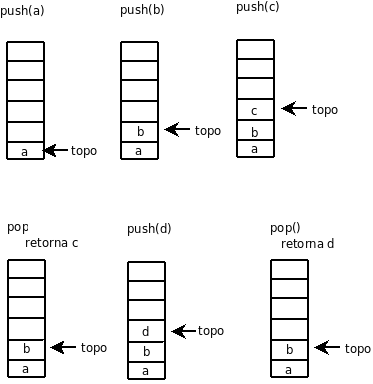
\includegraphics[width=.6\textwidth]{pilha}
			\end{figure} 
   \end{frame}
  
   \begin{frame}{Operações auxiliares}   
			\begin{itemize}
				\item Além das operações básicas, temos as operações ``\textit{auxiliares}''. São elas:
			\end{itemize}
			\begin{table}[ht]
			  \centering
						\begin{tabular}{l|l}
						    \hline \textbf{Operação} & \textbf{Descrição} \\
						    \hline create & cria uma pilha vazia.\\
						    \hline empty(p) & determina se uma pilha \textit{p} está ou não vazia.\\
						    \hline free(p) & libera o espaço ocupado na memória pela pilha \textit{p}.\\
						    \hline 
						\end{tabular}
						\caption{Operações auxiliares da estrutura de dados pilha.}
				\end{table}
  \end{frame}
  
\begin{frame}[fragile,plain]{Interface do Tipo Pilha -- Típica}
\begin{lstlisting}[language=C]
/* Definicao da estrutura */
typedef struct { DEFINA O SEU MODELO AQUI }  Pilha;

/*Aloca dinamicamente ou estaticamente a estrutura pilha, 
  inicializando seus campos e retorna seu ponteiro.*/
Pilha * create(void);

/*Insere o elemento e na pilha p.*/
void push(Pilha *p, int e);

/*Retira e retorna o elemento do topo da pilha p*/
int pop(Pilha *p);

/*Informa se a pilha p esta ou nao vazia.*/
int empty(Pilha *p);
\end{lstlisting}
\end{frame}



\begin{frame}
\frametitle{Implementações} 


\begin{enumerate}

  \item Baseada em um simples vetor
    \item Baseada em um vetor dinâmico
      \item Baseada em lista encadeada
      \pause
      \item mas todas usam ponteiros!


\end{enumerate}


\end{frame}


\begin{frame}{Implementação de Pilha com Vetor}  
	\begin{itemize}
		\item Normalmente as aplicações que precisam de uma 
		estrutura pilha, é comum saber de antemão o número 
		máximo de elementos que precisam estar armazenados 
		simultaneamente na pilha.
		\item Essa estrutura de pilha tem um limite conhecido.
		\item Os elementos são armazenados em um vetor.
		\item Essa implementação é mais simples.
		\item Os elementos inseridos ocupam as primeiras posições do vetor. 
	\end{itemize}
\end{frame}

\begin{frame}{Implementação de Pilha com Vetor}  
	\begin{itemize}
		\item Seja \textit{p} uma pilha armazenada em um vetor \textit{VET} de \textit{N} elementos:		
			\begin{enumerate}
				\item O elemento vet[topo] representa o elemento do topo.
				\item A parte ocupada pela pilha é vet[0 .. topo - 1].
				\item A pilha está vazia se topo = -1.
				\item Cheia se topo = N - 1.
				\item Para desempilhar um elemento da pilha, não vazia,
				 basta $$x = vet[topo--]$$ \textcolor{red}{(recupera valor do topo e depois decrementa)} 
				\item Para empilhar um elemento na pilha, em uma pilha não cheia, 
				basta $$vet[++t] = e$$   \textcolor{red}{(soma antes e depois insere)}
			\end{enumerate}
	\end{itemize}
\end{frame}

\begin{frame}[fragile]{Implementação de Pilha com Vetor}
\begin{lstlisting}[language=C]
#define N 20 /* numero maximo de elementos*/
#include <stdio.h>
#include "pilha.h"

/*Define a estrutura da pilha*/
struct pilha{
  int topo;            /* indica o topo da pilha */
  int elementos[N];   /* elementos da pilha*/
};

Pilha* create(void){
  Pilha* p = (Pilha * ) malloc(sizeof(Pilha));
  p->topo = -1;     /* inicializa a pilha com 0 elementos */
  return p;
}	
	\end{lstlisting}  
\end{frame}

\begin{frame}[fragile,c]{Implementação de Pilha com Vetor}
\begin{itemize}
	\item Empilha um elemento na pilha
\end{itemize}
\begin{lstlisting}[language=C]
void push(Pilha *p, int e){
     if (p->topo == N - 1){ /* capacidade esgotada */
        printf("A pilha esta cheia");
        exit(1);
     }
     /* insere o elemento na proxima posicao livre */
     p->elementos[++p->topo] = e;
}	
\end{lstlisting}  
\end{frame}

%%%
\begin{frame}[fragile,c]{Implementação de Pilha com Vetor}
\begin{itemize}
	\item Desempilha um elemento da pilha
\end{itemize}
\begin{lstlisting}[language=C]
int pop(Pilha *p)
{
     int e;
     if (empty(p)){
        printf("Pilha vazia.\n");
        exit(1);             
     } 
     
     /* retira o elemento do topo */
     e = p->elementos[p->topo--];
     return e;
}	
\end{lstlisting}  
\end{frame}


\begin{frame}[fragile]{Implementação de Pilha com Vetor}
\begin{lstlisting}[language=C]
/**
 * Verifica se a pilha p esta vazia
 */
int empty(Pilha *p)
{
   return (p->t == -1);
}

\end{lstlisting}
\end{frame}

\begin{frame}{Exemplos de Uso}
\begin{itemize}
	\item Na área computacional existem diversas aplicações de pilhas. 
	\item Alguns exemplos são: caminhamento em árvores, chamadas de sub-rotinas por um compilador ou pelo sistema operacional, inversão de uma lista, avaliar expressões, entre outras.
	\item Uma das aplicações clássicas é a conversão e a avaliação de expressões algébricas. Um exemplo, é o funcionamento das calculadoras da HP, que trabalham com expressões pós-fixadas.
\end{itemize}
\end{frame}






%\begin{frame}{Avaliação de Expressões}
%	\begin{itemize}
%		\item Considere as expressões aritméticas abaixo, e imagine que é nosso objetivo avaliar se as expressões estão definidas corretamente.		
%		\begin{enumerate}
%			\item (A + B) / C
%			\item 3 +  \{[2 + (7 * 3)/5] + (C - B)\} 
%		\end{enumerate}
%	\end{itemize}
%\end{frame}
%

\section{Aplicações -- Estudo de Casos}

\begin{frame}[c]{Balanceamento de Parenteses} 

		   	\begin{figure}[!htpb]
				\centering
				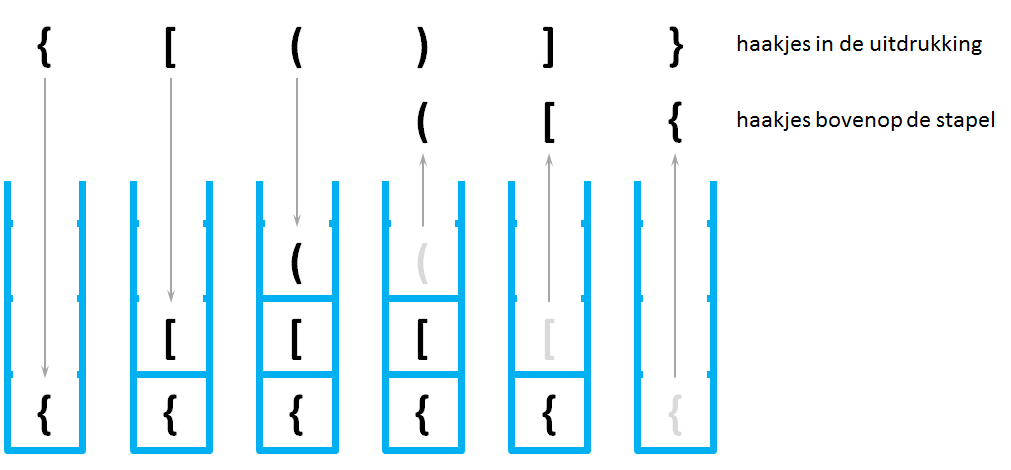
\includegraphics[width=.8\textwidth , height=.7\textheight]{parenteses_balanceado.png}
			\end{figure} 
\end{frame}


\begin{frame}[c]{Balanceamento de Parenteses} 

		   	\begin{figure}[!htpb]
				\centering
				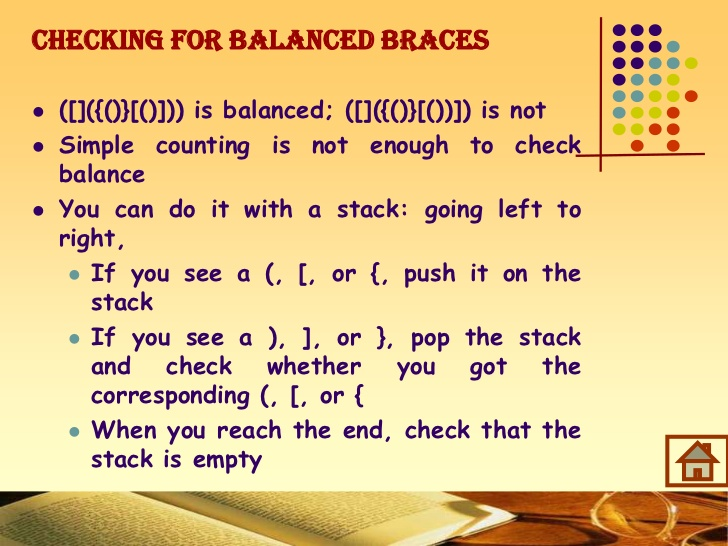
\includegraphics[width=.8\textwidth , height=.7\textheight]{alg_balanceamento.jpg}
			\end{figure} 
\end{frame}


\begin{frame}[c]{Validar Expressões Infixas} 

		   	\begin{figure}[!htpb]
				\centering
				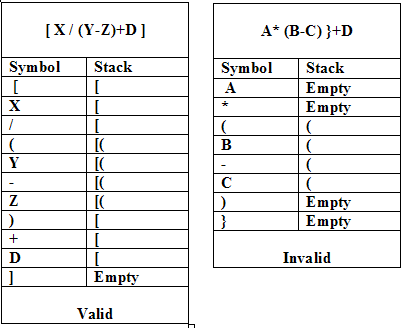
\includegraphics[width=.6\textwidth]{validar_expressoes.png}
			\end{figure} 
\end{frame}


\begin{frame}[c]{Conversão Pré-fixa para Pós-fixa} 

		   	\begin{figure}[!htpb]
				\centering
				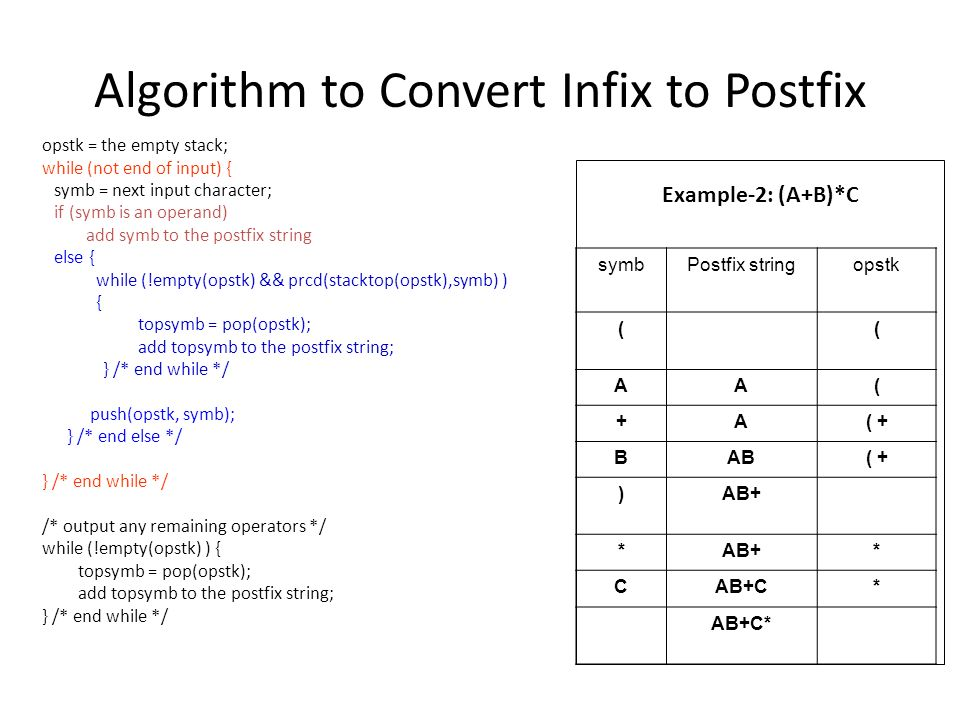
\includegraphics[width=.9\textwidth , height=.8\textheight]{infix_postfix00.jpg}
			\end{figure} 

\end{frame}



\begin{frame}[c]{Conversão Pré-fixa para Pós-fixa} 

		   	\begin{figure}[!htpb]
				\centering
				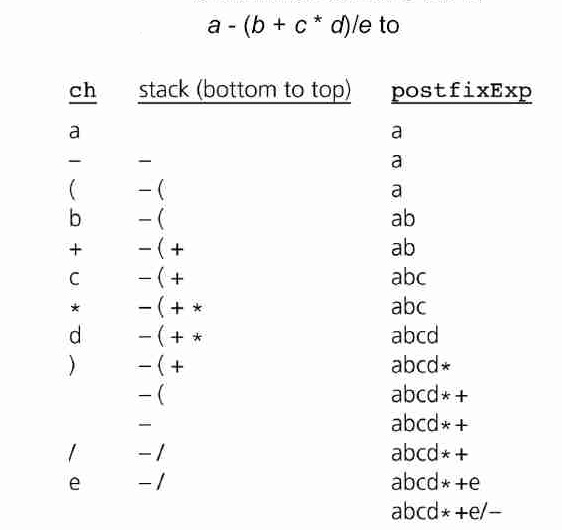
\includegraphics[width=.9\textwidth , height=.8\textheight]{infix_postfix01.jpg}
			\end{figure} 
\end{frame}



\begin{frame}[c]{Avaliação de Expressões Pós-fixas} 

		   	\begin{figure}[!htpb]
				\centering
				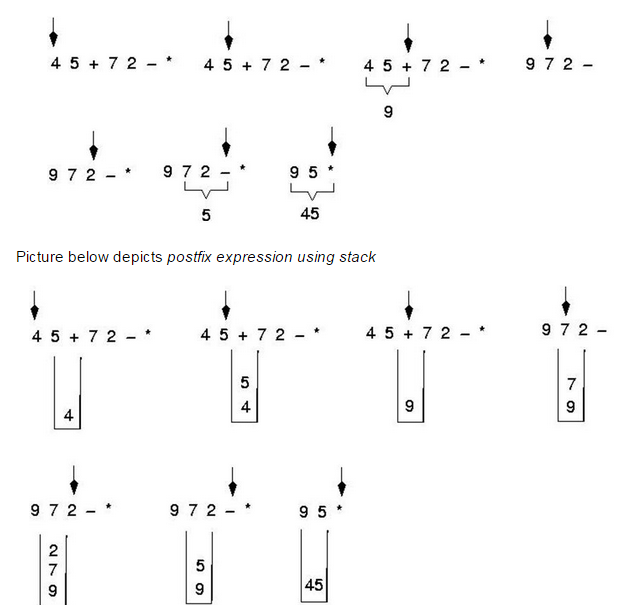
\includegraphics[width=.6\textwidth]{calcula_post_exp.png}
			\end{figure} 
\end{frame}


\begin{frame}[c]{DFS: Busca em Profundidade} 

		   	\begin{figure}[!htpb]
				\centering
				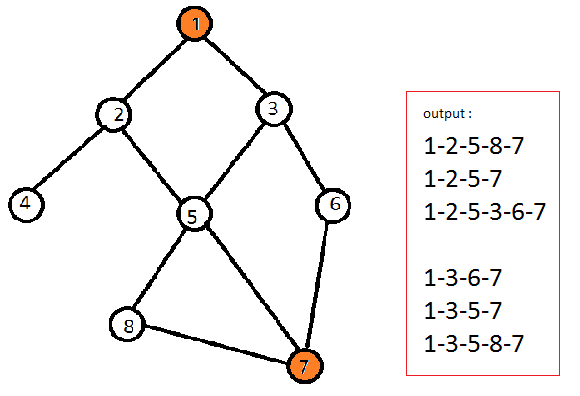
\includegraphics[width=.8\textwidth, height=.7\textheight]{grafo_visitas.png}
			\end{figure} 
\end{frame}



\begin{frame}[c]{DFS: Busca em Profundidade} 

		   	\begin{figure}[!htpb]
				\centering
				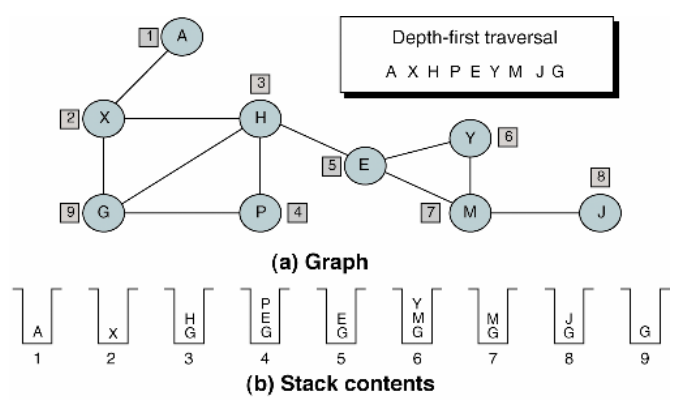
\includegraphics[width=.8\textwidth, height=.7\textheight]{dfs01.png}
			\end{figure} 
\end{frame}



\begin{frame}[c]{DFS: Busca em Profundidade} 

		   	\begin{figure}[!htpb]
				\centering
				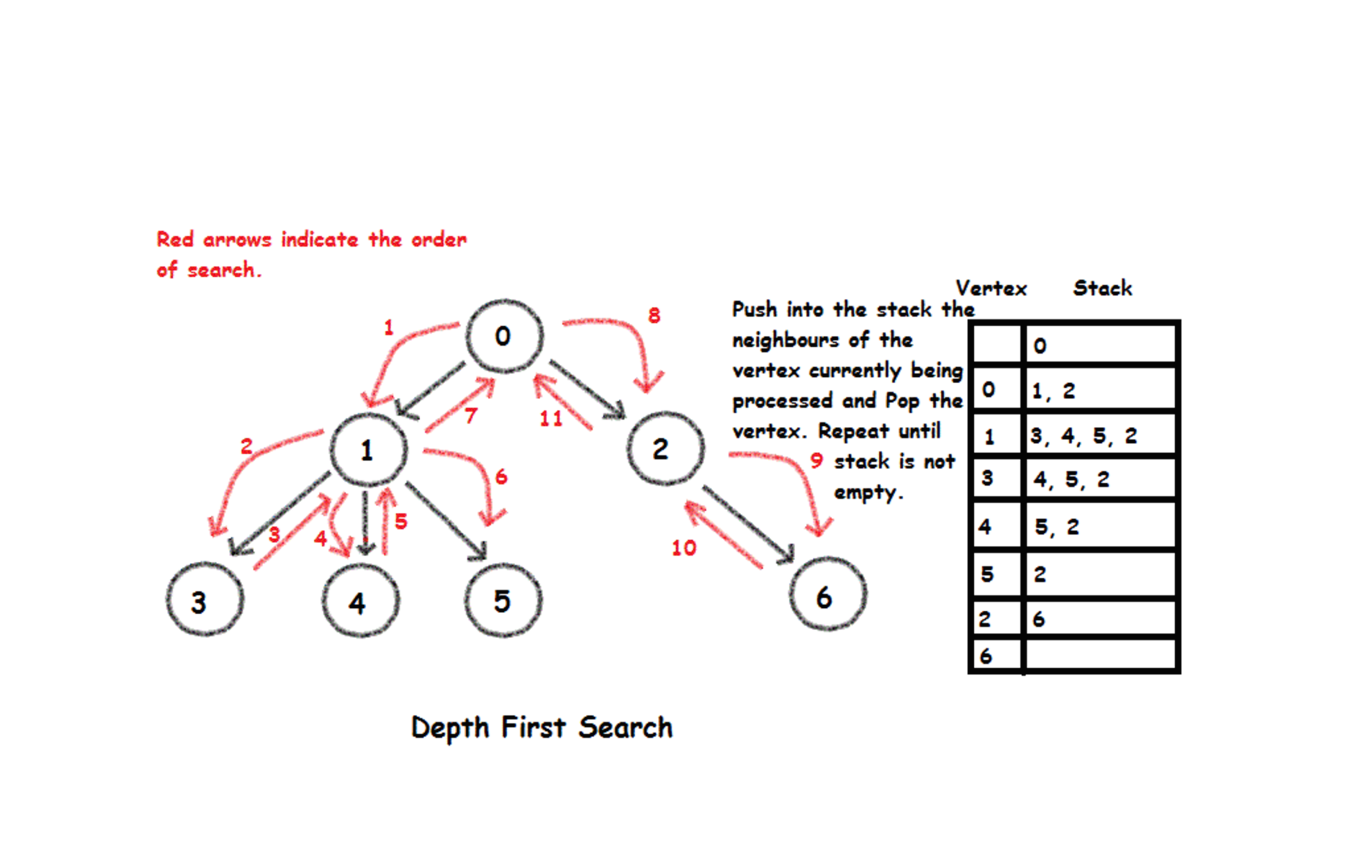
\includegraphics[width=.8\textwidth, height=.7\textheight]{dfs02.png}
			\end{figure} 
\end{frame}


\begin{frame}[c]{Representando Grafos: Matriz de Adjacência} 

		   	\begin{figure}[!htpb]
				\centering
				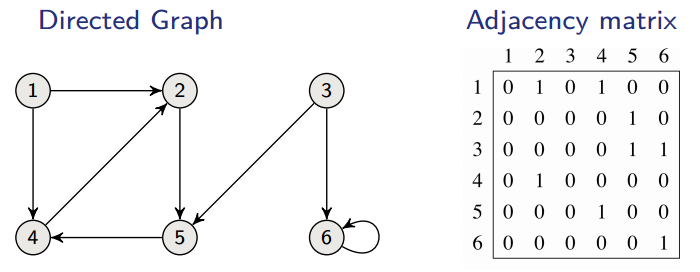
\includegraphics[width=.8\textwidth, height=.5\textheight]{adjacency-matrix.png}
			\end{figure} 
\end{frame}


\begin{frame}[c]{O Algoritmo DFS Iterativo} 

		   	\begin{figure}[!htpb]
				\centering
				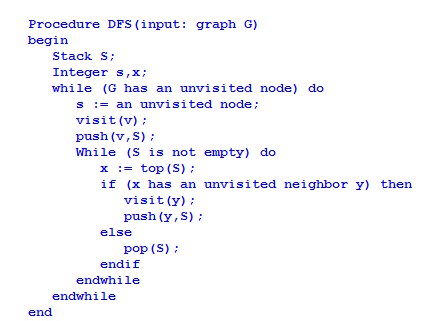
\includegraphics[width=.8\textwidth, height=.7\textheight]{depth-first-search-algorithm01.png}
			\end{figure} 
\end{frame}


\begin{frame}[c]{Ainda sobre o DFS} 

\begin{itemize}
  \item Veloz -- pouca memória
  \item Versátil: muitos tipos de aplicações
  \item Versão recursiva fica ainda mais simples
  \item Evita ciclos com os nós visitados 
  \item Veja a implementação usando pilhas
  
\end{itemize}

\end{frame}



\begin{frame}[fragile]{Exercícios}
	\begin{enumerate}
	
	\item Os exercícios propostos no início deste capítulo (slide inicial)
	
	
		\item Escreva uma função que inverta a ordem das letras de cada palavra de uma sentença, preservando a ordem das palavras. Suponha que as palavras da sentença são separadas por espaços. A aplicação da operação à sentença \textbf{AMU MEGASNEM ATERCES}, por exemplo, deve produzir \textbf{UMA MENSAGEM SECRETA}.
		\item Implemente uma função que receba uma pilha como parâmetro e retorne o valor armazenado em seu topo, restaurando o conteúdo da pilha. Essa função deve obedecer ao protótipo: 
		\begin{verbatim}
		   char topo(Pilha* p);
		\end{verbatim} 
		\item Implemente uma função que receba duas pilhas, $p_1, p_2$, e passe todos os elementos da pilha $p_2$ para o topo da pilha $p_1$. Essa função deve obedecer ao protótipo: 
		\begin{verbatim}
		   void concatena(Pilha* p1, Pilha* p2);
		\end{verbatim} 
	\end{enumerate}
\end{frame}
 % cap 2
%!TEX root = curso_EDA_SLIDES.tex
%!TeX spellcheck = pt_BR
\section{Filas}

\begin{frame}

\begin{center}
{\Large Capítulo 03 -- Filas}
\end{center}

\begin{columns}
\begin{column}{.4\textwidth}
\centering
Pontos fundamentais a serem cobertos:
  \begin{enumerate}
  \item Contexto e motivação
  \item Definição
  \item Implementações
  \item Exercícios 
\end{enumerate}  

\end{column}

\begin{column}{.6\textwidth}
\centering
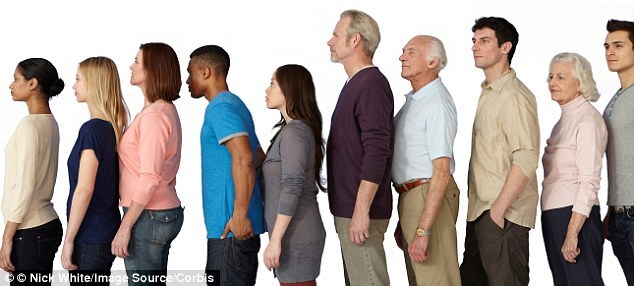
\includegraphics[height=4cm, width=7cm]{figs/fig_filas/fila_pessoas.jpeg}
%\hspace{+0.25cm}
%\scriptsize\textcolor{red}{[Tizio, Caio et al., Nature (2006)]}
\end{column}

\end{columns}


\end{frame}
%-----------------------------------------------------------------------


  \begin{frame}{Introdução}    

		\begin{itemize}
			\item Assim como a estrutura de dados Pilha, Fila é outra estrutura de dados 
			bastante utilizada em computação.
			\item Um exemplo é a implementação de uma fila de impressão.
			\item Se uma impressora é compartilhada por várias máquinas, 
			normalmente adota-se uma estratégia para determinar a ordem de impressão dos documentos.
			\item A maneira mais simples é tratar todas as requisições 
			com a mesma prioridade e imprimir os documentos na ordem em que 
			foram submetidos -- o primeiro submetido é o primeiro a ser impresso.
		\end{itemize}
  \end{frame}

%-----------------------------------------------------------------------
  
\begin{frame}{Fila}
     \begin{block}{Aplicações}

\begin{enumerate}
  \item Escalonamento de processos na CPU (processos com a mesma prioridade)
        os quais são executados em ordem de chegada
  \item Simulação de filas no mundo real tais como: filas em banco, compra de tickets, etc
  
  \item Multi-programação
  \item Transferência assíncrona de dados (IO de arquivos, pipe, sockets)
  \item Fila de espera em um \textit{call-center}      
  \item Encontrar número de atendentes em supermercados e caixas bancários dado uma
  demanda de pessoas na sala de espera
  
\end{enumerate}
     \end{block}          
\end{frame}


%-----------------------------------------------------------------------
  
\begin{frame}{Fila}
     \begin{block}{Aplicações Indiretas}

\begin{enumerate}
  \item Estrutura de dados auxiliares em algoritmos
  \item Componente de outras estruturas
\end{enumerate}
     \end{block}          
\end{frame}

%-----------------------------------------------------------------------
  
\begin{frame}{Fila}
     \begin{block}{Definição}
       Um conjunto ordenado de itens a partir do qual podem-se eliminar 
       itens numa extremidade (chamada de \alert{início} da fila) e
        no qual podem-se inserir itens na outra extremidade 
        (chamada \alert{final} da fila).
     \end{block}          
\end{frame}

%-----------------------------------------------------------------------

\begin{frame}{Representação}

\begin{itemize}
	\item Os nós de uma fila são armazenados em endereços contínuos.	
	\item A Figura~\ref{fig:fila-representacao} ilustra uma fila com três elementos.
\end{itemize}

\begin{figure}[ht!]
				\centering
				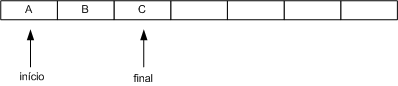
\includegraphics[width=.6\textwidth]{figs/fig_filas/exemplo_fila_tres_elementos.png}
				\caption{Exemplo de representação de fila.}
				\label{fig:fila-representacao}
			\end{figure} 

\begin{itemize}
	\item Após a retirada de um elemento (\textit{primeiro}) temos:

\end{itemize}

	\begin{figure}[hb!]
					\centering
				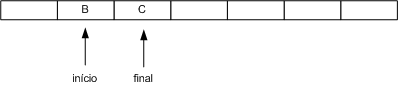
\includegraphics[width=.6\textwidth]{figs/fig_filas/exemplo_fila_tres_retirada.png}
				\caption{Representação de uma fila após a remoção do elemento ``A''.}	
	\end{figure} 

 \end{frame}
%-----------------------------------------------------------------------

\begin{frame}{Implementações}

\begin{block}{Quais as estruturas usadas por filas?}
  \begin{itemize}
    \item Baseada num vetor simples -- limitada
    \item Baseada num vetor circular simples -- limitada
    \item Baseada num vetor circular dinâmico -- \textbf{i}limitada
    \item Baseada numa lista encadeada (depois de listas)
    
  \end{itemize}
\end{block}

\end{frame}


%------------------------------------
\begin{frame}{Representação}
\begin{itemize}
	\item Após a inclusão de dois elementos temos:
	\begin{figure}[ht]
				\centering
				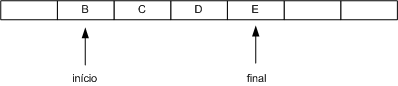
\includegraphics[width=.6\textwidth]{figs/fig_filas/exemplo_fila_tres_inclusao.png}
				\caption{Representação de uma fila após a inclusão de dois elementos ``D'' e ``E''.}	
			\end{figure} 
\end{itemize}

\begin{itemize}

	\item Como podemos observar, a operação de inclusão e retirada de um item da fila incorre na mudança do endereço do ponteiro que informa onde é o início e o término da fila.
\end{itemize}

\end{frame}







\begin{frame}[fragile]{Representação}
\begin{itemize}
	\item Em uma fila, o \alert{primeiro} elemento inserido é o primeiro a ser removido.
	\item Por essa razão, uma fila é chamada \textbf{\alert{fifo(\textit{first-in first-out})}} -- primeiro que entra é o primeiro a sair -- ao contrário de uma pilha que é \alert{lifo} (\textit{last-in, first-out})
	\item Para exemplificar a implementação em C, vamos considerar que o conteúdo armazenado na fila é do tipo inteiro.
	\item A estrutura de fila possui a seguinte representação:	
\end{itemize}
\footnotesize
\begin{lstlisting}[language=C]
  struct fila{
    int elemento[N];
    int ini, n;
  }
  typedef struct fila Fila;
\end{lstlisting}

\begin{itemize}
	\item Trata-se de uma estrutura heterogênea constituída de membros distintos entre si.
	 Os membros são as variáveis \alert{\textit{ini}} e \alert{\textit{fim}}, que serve para armazenar respectivamente, o início e o fim da fila e o vetor \alert{\textit{elemento}} 
	 de inteiros que armazena os itens da fila.
\end{itemize}
\end{frame}


\begin{frame}{Operações Primitivas}
  \begin{itemize}
	  \item As operações básicas que devem ser implementadas em uma estrutura do tipo Fila são:		
  \end{itemize}
  \begin{table}[ht]
			  \centering
						\begin{tabular}{l|l}
						    \hline \textbf{Operação} & \textbf{Descrição} \\
						    \hline criar() & aloca dinamicamente a estrutura da fila.\\
						    \hline insere(f,e) & adiciona um novo elemento \textit{(e)}, no final da fila \textit{f}.\\
						    \hline retira(f) & remove o elemento do início da fila \textit{f}.\\						   
						    %\hline pesquisar(f,e) & pesquisa o elemento \textit{e} na fila \textit{f}.\\
						    \hline 
						\end{tabular}
						\caption{Operações básicas da estrutura de dados fila.}
				\end{table}
\end{frame}
 
\begin{frame}{Operações auxiliares}   
			\begin{itemize}
				\item Além das operações básicas, temos as operações ``auxiliares''. São elas:
			\end{itemize}
			\begin{table}[ht]
			  \centering
						\begin{tabular}{l|l}
						    \hline \textbf{Operação} & \textbf{Descrição} \\						    
						    \hline vazia(f) & informa se a fila está ou não vazia.\\
						    \hline libera(f) & destrói a estrutura, e assim libera toda a memória alocada.\\
						    \hline 
						\end{tabular}
						\caption{Operações auxiliares da estrutura de dados fila.}
				\end{table}
  \end{frame}


\begin{frame}[fragile,plain]{Interface do Tipo Fila}
\footnotesize
\begin{lstlisting}[language=C]
typedef struct fila Fila;
/* Aloca dinamicamente a estrutura Fila, inicializando seus
 * campos e retorna seu ponteiro. A fila depois de criada
 * estarah vazia.*/
Fila* criar(void);

/* Insere o elemento e no final da fila f, desde que,
 * a fila nao esteja cheia.*/
void insere(Fila* f, int e);

/* Retira o elemento do inicio da fila, e fornece o 
 * valor do elemento retirado como retorno, desde que a fila
 * nao esteja vazia*/
int retira(Fila* f);

/*Verifica se a fila f estah vazia*/
int vazia(Fila* f);

/*Libera a memoria alocada pela fila f*/
void libera(Fila* f);
\end{lstlisting}
\end{frame}

\begin{frame}{Implementação de Fila com Vetor}
	\begin{itemize}
		\item Assim como nos casos da pilha e lista, a implementação de fila será feita usando um vetor para armazenar os elementos.
		\item Isso implica, que devemos fixar o número máximo de elementos na fila.
		\item O processo de inserção e remoção em extremidades opostas fará a fila ``andar'' no vetor.
		\item Por exemplo, se inserirmos os elementos 8, 7, 4, 3 e depois retiramos dois elementos, a fila não estará mais nas posições iniciais do vetor.
	\end{itemize}
	\begin{figure}[ht]
				\centering
				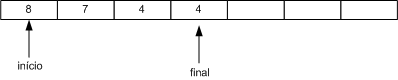
\includegraphics[width=.6\textwidth]{fila_insercao_quatro_elementos.png}
				\caption{Fila após inserção de quatro elementos.}	
	\end{figure} 	
\end{frame}

\begin{frame}{Implementação de Fila com Vetor}	
	\begin{figure}[ht]
				\centering
				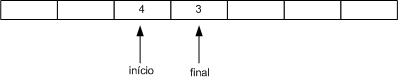
\includegraphics[width=.6\textwidth]{exemplo_fila_remove_dois_elementos.png}
				\caption{Fila após retirar dois elementos.}	
	\end{figure} 	
	\begin{itemize}
		\item Com essa estratégia, é fácil observar que, em um dado instante, a parte ocupada pelo vetor pode chegar a última posição.
		\item Uma solução seria ao remover um elemento da fila, deslocar a fila inteira no sentido do início do vetor.
		\item Entretanto, essa método é bastante ineficiente, pois cada retirada implica em deslocar cada elemento restante da fila. Se uma fila tiver 500 ou 1000 elementos, evidentemente esse seria um preço muito alto a pagar.		
	\end{itemize}
\end{frame}

\begin{frame}{Implementação de Fila com Vetor}		
	\begin{itemize}		
		\item Para reaproveitar as primeira posições do vetor sem implementar uma ``re-arrumação'' dos elementos, podemos incrementar as posições do vetor de forma ``circular''.
		\item Para essa implementação, os índices do vetor são incrementados de maneira que seus valores progridam ``circularmente''. 
		\item Dessa forma, se temos 100 posições no vetor, os índices assumem os seguintes valores:
		$$0, 1, 2, 3, \cdots, 98, 99, 0, 1, 2, 3, \cdots, 98, 99, \cdots$$
	\end{itemize}
\end{frame}



%-----------------------------

\begin{frame}{Porquê um \textit{vetor circular}?}

\begin{block}{Reflexões}
  \begin{itemize}
    \item Tamanho fixo -- muito interessante para maioria dos problemas
    \item Velocidade
    \item Fácil de manipular
    \item \textit{Circular} é a manipulação!
    
    
  \end{itemize}
\end{block}

\end{frame}

%------------------------------------------------
\begin{frame}{\textit{Vetor} Circular: Explicações}

\begin{figure}[ht!]
				\centering
				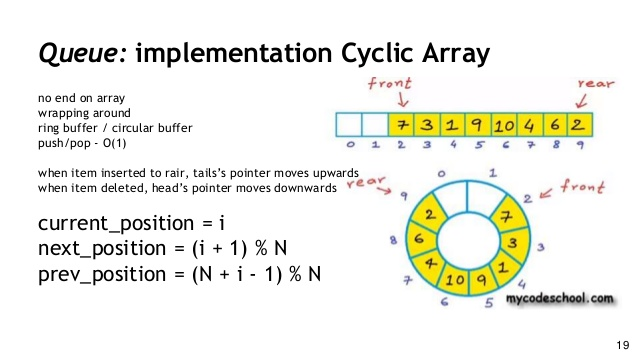
\includegraphics[width=.8\textwidth,height=.6\textheight]{figs/fig_filas/fila_circular_explicacao_01.jpg}
		%	\caption{Exemplo de representação de fila.}
			%	\label{fig:fila-representacao}
			\end{figure} 

\end{frame}

\begin{frame}{\textit{Vetor} Circular: Explicações}

\begin{figure}[ht!]
			\centering
			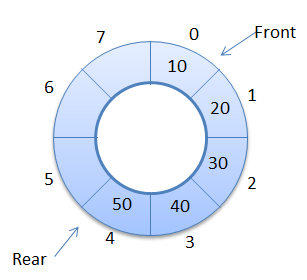
\includegraphics[width=.5\textwidth]{figs/fig_filas/fila_circular_simples.png}
		\caption{Notação aqui empregada}
			%	\label{fig:fila-representacao}
			\end{figure} 
\end{frame}


\begin{frame}{\textit{Vetor} Circular: Explicações}

\begin{figure}[ht!]
	\centering
		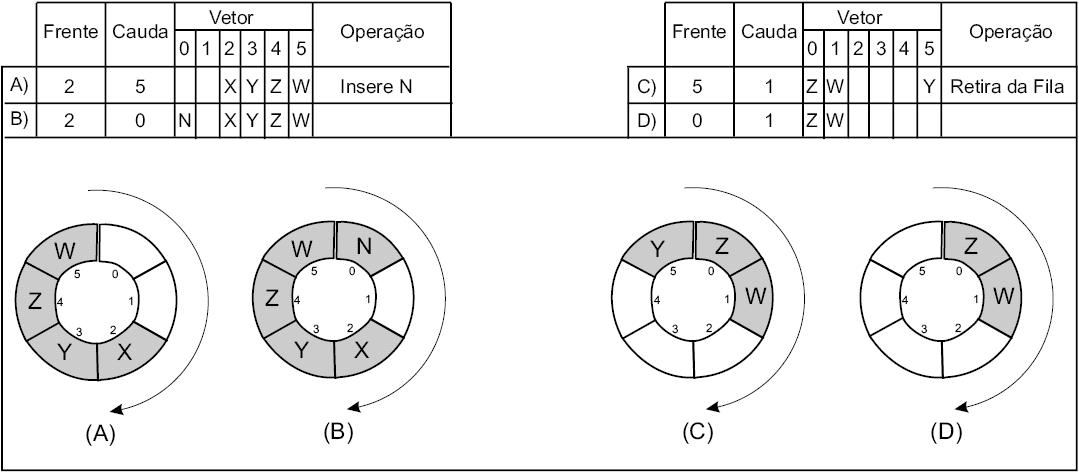
\includegraphics[width=.8\textwidth,height=5cm]{figs/fig_filas/fila_circular_explicacao_02.jpg}
		%	\caption{Exemplo de representação de fila.}
			%	\label{fig:fila-representacao}
			\end{figure} 
\end{frame}


\begin{frame}[fragile]{Função de Criação}
	\begin{itemize}
		\item A função que cria uma fila, deve criar e retornar o ponteiro de uma fila vazia

		\item A função deve informar onde é o início da fila, ou seja, fazer \texttt{f->ini = 0}, 
		como podemos ver no código abaixo
		
		\item A complexidade de tempo para criar a fila é constante, ou seja, $O(1)$
	\end{itemize}
\small	
\begin{lstlisting}[language=C]
/* Aloca dinamicamente a estrutura Fila, inicializando seus
 * campos e retorna seu ponteiro. A fila depois de criada
 * estarah vazia.
 */
Fila* criar(void)
{
   Fila* f = malloc(sizeof(Fila));
   f->n = 0; // quantidade CORRENTE elementos
   f->ini = 0; // inicio
   return f;
}
\end{lstlisting}
\end{frame}

\begin{frame}[fragile]{Função de Inserção}  
	\begin{itemize}
		\item Para inserir um elemento na fila, usamos a próxima posição 
		livre do vetor, indicada por \alert{n}.
		\item Devemos assegurar que há espaço para inserção do novo 
		elemento no vetor, haja vista se tratar de um vetor com capacidade limitada. 
		\item A complexidade de tempo para inserir um elemento na fila 
		é constante, ou seja, $O(1)$.
	\end{itemize}
\footnotesize
\begin{lstlisting}[language=C]
/* Insere o elemento e no final da fila f.*/
void insere(Fila* f, int e)
{
  int fim;
  if (f->n == N){
     printf("Fila cheia!\n"); }
  else{
     fim = (f->ini + f->n) % N;
     f->elementos[fim] = e;  
     f->n++;
  }
}
\end{lstlisting}	
\end{frame}

\begin{frame}[fragile]{Função de Remoção} 
	\begin{itemize}
		\item A função para retirar o elemento do 
		início da fila fornece o valor do elemento retirado 
		como retorno.
		\item Para remover um elemento, devemos verificar se 
		a fila está ou não vazia.
		\item A complexidade de tempo para remover 
		um elemento da fila é constante, ou seja, $O(1)$.
	\end{itemize}
	
\footnotesize
\begin{lstlisting}[language=C]
int retira(Fila* f)
{
  int e;
  if ( vazia(f) )
    printf("Fila vazia!\n");
  else{
    e = f->elementos[f->ini];
    f->ini = (f->ini + 1) % N;
    f->n--;
  }
  return e;
}
\end{lstlisting}	
\end{frame} 

%\begin{frame}[fragile]{Função de Pesquisa} 
%	\begin{itemize}
%		\item Para pesquisar um elemento qualquer na lista é necessário compará-lo com os elementos existentes, utilizando alguns dos algoritmos de busca conhecidos;
%		\item A complexidade de tempo dessa função depende do algoritmo de busca implementado. Se utilizarmos a busca seqüencial, a complexidade da função será $O(n)$. No entanto, é possível baixá-lo para $O(n\log n)$, utilizando alguns dos algoritmos mais refinados.
%\end{itemize}
%
%\footnotesize
%\begin{verbatim}
%}\end{verbatim}
%\end{frame}

\begin{frame}[fragile]{Exemplo de Uso da Fila}

\begin{footnotesize}

\begin{lstlisting}[language=C]
#define N 10
#include <stdio.h>
#include "fila.h"  // TDA.h

int main(void)
{
    Fila * f = criar();
    
    int i;
    for (i = 0; i < N; i++)
      insere(f, i * 2);
      
    printf("\nElementos removidos: ");
      
    for (i = 0; i < N/2; i++)
     printf("%d ", retira(f)); 
               
}
\end{lstlisting}
\end{footnotesize}
\end{frame} 


\begin{frame}{Exercícios}
	
	\begin{enumerate}
	\item
	\item
	\item
	
	\end{enumerate}
	
\end{frame}





\begin{frame}{Referências}
	
	\begin{enumerate}
		\item Tenenbaum, A. M., Langsam, Y., and Augestein, M. J. (1995). 
		\textit{Estruturas de Dados Usando C}. MAKRON Books, pp. 207-250.
		\item Wirth, N. (1989). \textit{Algoritmos e Estrutura de Dados}. LTC, pp. 151-165.
	
	\end{enumerate}
	
\end{frame}
 % cap 3

\section{Listas}

\begin{frame}

\begin{center}
{\Large Capítulo 05 -- Listas}
\end{center}

\begin{columns}
\begin{column}{.5\textwidth}
\centering
Pontos fundamentais a serem cobertos:
  \begin{enumerate}
  \item Contexto e motivação
  \item Definição
  \item Implementações
  \item Exercícios 
\end{enumerate}  

\end{column}
\begin{column}{.5\textwidth}
\centering
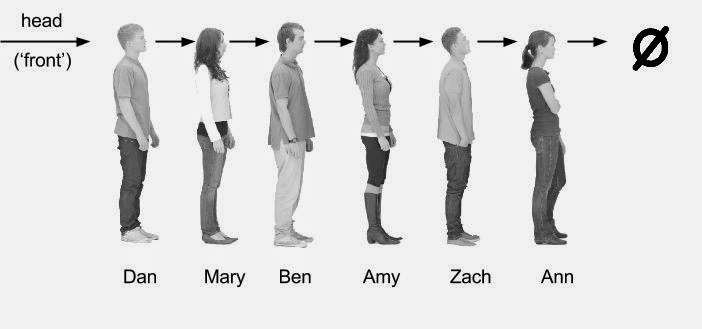
\includegraphics[height=2.5cm, width=7cm]{figs/fig_listas/ilustra_lista.jpg}
%\hspace{+0.25cm}
%\scriptsize\textcolor{red}{[Tizio, Caio et al., Nature (2006)]}
\end{column}
\end{columns}


\end{frame}
%----------------------------------------------------------------------------------------------------------
\begin{frame}

\begin{block}{ \textcolor{red}{Atenção:} }

\begin{itemize}
  \item \textcolor{red}{Duas partes este capítulo}
  \item   Listas com um vetor de tamanho fixo internamente
  \item  Listas estruturadas em nós alocados dinamicamente
  \item  Conceitualmente, equivalentes!
  \item  Implementações discutidas: alocação dinâmica!
  \item  Aqui justifica-se o estudo extensivo de ponteiros no início do curso
\end{itemize}

\end{block}

\end{frame}
%----------------------------------------------------------------------------------------------------------


%----------------------------------------------------------------------------------------------------------

\subsection{Listas -- Tamanho Limitado}
  \begin{frame}{Introdução}    
		\begin{itemize}
			\item Uma seqüência de nós ou elementos dispostos em uma ordem estritamente linear.
			\item Cada elemento da lista é acessível um após o outro, em ordem.
			\item Pode ser implementada de várias maneiras			
				\begin{enumerate}
					\item Em um vetor
					\item Em uma estrutura que tem um vetor de tamanho fixo e uma 
					variável para armazenar o tamanho da lista
					\item Conjunto de nós criados e ligados dinâmicamente (abordagem aqui adotada nos códigos apresentados)
					\pause
					\item As duas implementações iniciais são exercícios de disciplinas anteriores.
				\end{enumerate}
		\end{itemize}
  \end{frame}

%----------------------------------------------------------------------------------------------------------
  \begin{frame}{Motivação}    
	\begin{enumerate}
	\item Talvez a estrutura de dados mais importante
	\item Generaliza Pilhas e Filas
	\item Utilizada em várias outras estruturas como grafos e árvores
	\pause
	\item Os exemplos em código apresentados, utilizam extensivamente 
	endereçamentos de memória (ponteiros e ponteiros para ponteiros) e alocações dinãmicas
	de memória
	\item Contudo, para fins conceitual usaremos uma lista {\em rígida} nestes slides
	\end{enumerate}
	
  \end{frame}
%----------------------------------------------------------------------------------------------------------
\begin{frame}{Aplicações}    
	\begin{enumerate}
	\item 
	\pause
	\item 
	\end{enumerate}
	
  \end{frame}
%----------------------------------------------------------------------------------------------------------

\begin{frame}
\frametitle{Exemplo de Uso}
\begin{figure}[!hb]
	\centering
		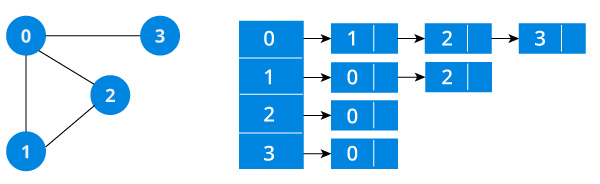
\includegraphics[height=0.30\paperheight, width=0.55\paperwidth]{figs/fig_listas/lista_matriz_adjacencia}			
			\caption{Uso de lista para representar matriz de adjacência}	
%%				\label{fig:lista-linear-repre}
			\end{figure} 

  \end{frame}
%----------------------------------------------------------------------------------------------------------



%----------------------------------------------------------------------------------------------------------  
\begin{frame}{Definição}
     \begin{block}{Definição}
     \begin{itemize}
       \item Um conjunto de nós, $x_1, x_2, x_3, \cdots, x_n$, organizados estruturalmente de forma a refletir as posições relativas dos mesmos. 
       \item  Se $n > 0$, então $x_1$ é o primeiro nó.
      \item Seja $L$ uma lista de $n$ nós, e $x_k$ um nó $\in$ L e $k$ a posição do nó em $L$. 
      \item  Então, $x_k$ é precedido pelo nó $x_{k-1}$ e seguido pelo nó $x_{k+1}$. 
      \item  O último nó de $L$ é $x_{n-1}$. Quando $n = 0$, dizemos que a lista está vazia.
       \end{itemize}
     \end{block}     
\end{frame}
%----------------------------------------------------------------------------------------------------------



%----------------------------------------------------------------------------------------------------------
\begin{frame}{Representação}
\begin{itemize}
	\item Os nós de uma lista são armazenados em {\it endereços contínuos} (apenas os endereços)
	\item A relação de ordem é representada pelo fato de que se o endereço do 
	nó $x_i$ é conhecido, então o endereço do nó $x_{i+1}$ também pode ser determinado. 	
	\item A Figura \ref{fig:lista-linear-repre} apresenta a representação de
	 uma lista linear de $n$ nós, com endereços representados por $k$
\end{itemize}

\begin{figure}[hb]
	\centering
		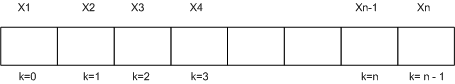
\includegraphics[width=.6\textwidth]{figs/fig_listas/lista-linear.png}			
			\caption{Exemplo de representação de lista -- usando um vetor}	
				\label{fig:lista-linear-repre}
			\end{figure} 
\end{frame}
%----------------------------------------------------------------------------------------------------------
\begin{frame}[fragile,c]{Representação com um Vetor de Inteiros}
\begin{itemize}
	\item Para exemplificar a implementações em C, vamos considerar que 
	o conteúdo armazenado na lista é do tipo inteiro (nos códigos são {\it strings}).
	\item A estrutura da lista possui a seguinte representação:	
\end{itemize}
\begin{lstlisting}[language=C]
  struct lista{
    int cursor;
    int elemento[N];
  }
  typedef struct lista Lista;
\end{lstlisting}

\begin{itemize}
	\item Trata-se de uma estrutura heterogênea constituída de membros distintos entre si. 
	\item Os membros são as variáveis \alert{\textit{cursor}}, que serve para armazenar a 
	quantidade de elementos da lista e o vetor \alert{\textit{elemento}} de inteiros
	que armazena os nós da lista.
	\item Até o momento uma alocação estática
\end{itemize}
\end{frame}
%----------------------------------------------------------------------------------------------------------

\begin{frame}[fragile,c]{Representação Estática -- Tamanho Fixo}
\begin{itemize}

 \item Para atribuirmos um valor a algum membro da lista devemos utilizar a seguinte notação:

\small	
\begin{lstlisting}[language=C]
Lista->elemento[0] = 1 //atribui o valor 1 ao primeiro elemento da lista.
Lista->elemento[n-1] = 4 //atribui o valor 4 ao ultimo elemento da lista.
\end{lstlisting}
\end{itemize}
\end{frame}  
%----------------------------------------------------------------------------------------------------------

\begin{frame}{Operações Primitivas}
  \begin{itemize}
	  \item As operações básicas que devem ser implementadas em uma estrutura do tipo Lista são:		
  \end{itemize}
  \begin{table}[!htpb]
	\centering
    \begin{tabular}{l|l}
	 \hline \hline 
	 \textbf{Operação} & \textbf{Descrição} \\
	\hline \hline \\
	criar() & cria uma lista vazia.\\
	 \hline inserir(l,e) & insere o elemento \textit{e} no final da lista \textit{l}.\\
	 \hline remover(l,e) & remove o elemento \textit{e} da lista \textit{l}.\\
	\hline imprimir(l) & imprime os elementos da lista \textit{l}.\\
	\hline pesquisar(l,e) & pesquisa o elemento \textit{e} na lista \textit{l}.\\
	\hline 	\hline 
	\end{tabular}
	\caption{Operações básicas da estrutura de dados lista.}
\end{table}
\end{frame}
%----------------------------------------------------------------------------------------------------------
 
\begin{frame}{Operações auxiliares}   
	\begin{itemize}
	\item Além das operações básicas, temos as operações ``auxiliares''. São elas:
	\end{itemize}
	\begin{table}[!htpb]
	  \centering
	\begin{tabular}{l||l}
	    \hline \hline 
	 \textbf{Operação} & \textbf{Descrição} \\
	\hline \hline \\
	    \hline empty(l) & determina se a lista \textit{l} está ou não vazia.\\
	    \hline destroy(l) & libera o espaço ocupado na memória pela lista \textit{l}.\\
	    \hline \hline
	\end{tabular}
\caption{Operações auxiliares da estrutura de dados lista.}
\end{table}
 \end{frame}
 
%----------------------------------------------------------------------------------------------------------

\begin{frame}[fragile,plain]{Interface do Tipo Lista}
\footnotesize
\begin{lstlisting}[language=C]
/* Aloca dinamicamente a estrutura lista, inicializando 
 * seus campos e retorna seu ponteiro. A lista depois 
 * de criada terah tamanho igual a zero. Sem malloc ... ainda */
Lista* criar(void);

/* Insere o elemento e no final da lista l, desde que,
 * a lista nao esteja cheia ... dada a limitacao inicial */
void inserir(Lista* l, int e);

/* Remove o elemento e da lista l,
 * desde que a lista nao esteja vazia e o elemento
 * e esteja na lista. A funcao retorna 0 se o elemento 
 * nao for encontrado na lista ou 1 caso contrario. */
void remover(Lista* l, int e);

/* Pesquisa na lista l o elemento e. A funcao retorna 
 * o endereco(indice) do elemento se ele pertencer a lista
 * ou -1 caso contrario.*/
int pesquisar(Lista* l, int e);

/* Lista os elementos da lista l. */
void imprimir(Lista* l);
\end{lstlisting}
\end{frame}
%----------------------------------------------------------------------------------------------------------

\begin{frame}{Implementação das Listas de Tamanho Fixo}

A utilização de vetores para implementar a lista traz algumas vantagens como:	
  \begin{enumerate}
	\item Os elementos são armazenados em posições contíguas da memória
	\item Basta ver a estrutura, internamente é um vetor
	\item Economia de memória, pois os ponteiros para o próximo elemento da lista são explícitos
	\item Há um índice de acesso direto e o {\em cursor} para indicar o último elemento
\end{enumerate}

\end{frame}

%----------------------------------------------------------------------------------------------------------
\begin{frame}{Implementação das Listas de Tamanho Fixo}

No entanto, as desvantagens são:		
  \begin{enumerate}
\item Custo de inserir/remover elementos da lista 
\pause
\item Neste caso se refere ao deslocamento células a frente no caso de inserção
\pause
\item ou  deslocamento células para trás no caso de remoção
\pause
\item Finalmente: limitação da quantidade de elementos da lista
\item Este é ponto ... tamanho fixo!
\item Aqui, usamos alocação dinâmica, mas todos conceitos aqui são complementares
\end{enumerate}

\end{frame}
%----------------------------------------------------------------------------------------------------------

\begin{frame}[fragile,c]{Função de Criação}
	\begin{itemize}
	\item A função que cria uma lista, deve criar e retornar uma lista vazia;
	\item A função deve atribuir o valor zero ao tamanho da lista, ou seja, fazer $l->cursor = 0$, como podemos ver no código abaixo.
	\item A complexidade de tempo para criar a lista é constante, ou seja, $O(1)$.
	\end{itemize}
	
\begin{lstlisting}[language=C]
/*
 * Aloca dinamicamente a estrutura lista, inicializando seus
 * campos e retorna seu ponteiro. A lista depois de criada
 * terah tamanho igual a zero.
 */
Lista* criar(void){
  Lista* l = (Lista*) malloc(sizeof(Lista));
  l->cursor = 0;
  return l;
}
\end{lstlisting}
\end{frame}
%----------------------------------------------------------------------------------------------------------

\begin{frame}[fragile,c]{Função de Inserção}  
	\begin{itemize}
	\item A inserção de qualquer elemento ocorre no final da lista, desde que a lista não esteja cheia.
	\item Com isso, para inserir um elemento basta atribuirmos o valor ao elemento cujo índice é o valor referenciado pelo campo \textit{cursor}, e incrementar o valor do cursor, ou seja fazer 
	\texttt{l->elemento[l->cursor++] = valor}, como podemos verificar no código abaixo, a uma complexidade de tempo constante, $O(1)$.
	\end{itemize}

\footnotesize
\begin{lstlisting}[language=C]
/*
 * Insere o elemento e no final da lista l, desde que,
 * a lista nao esteja cheia.
 */
void inserir(Lista* l, int e){
  if (l == NULL || l->cursor == N){
    printf("Error. A lista esta cheia\n");
  }else{
    l->elemento[l->cursor++] = e;
  }
}
\end{lstlisting}	
\end{frame}
%----------------------------------------------------------------------------------------------------------

\begin{frame}[fragile,c]{Função de Remoção} 
	\begin{itemize}
		\item Para remover um elemento da lista, primeiro precisamos verificar se ele está na lista, para assim removê-lo, e deslocar os seus sucessores, quando o elemento removido não for o último.
		\item A complexidade de tempo da função de remoção é $O(n)$, pois é necessário movimentar os $n$ elementos para remover um elemento e ajustar a lista.
	\end{itemize}
	
\footnotesize
\begin{lstlisting}[language=C]
/* remove um elemento da lista */
void remover(Lista* l, int e){     
  int i, d = pesquisar(l,e);
  if (d != -1){
    for(i = d; i < l->cursor; i++)
    {
      l->elemento[i] = l->elemento[i + 1];
    }
    l->cursor--;
  }  
}
\end{lstlisting}	
\end{frame} 
%----------------------------------------------------------------------------------------------------------

\begin{frame}[fragile]{Função de Pesquisa} 
   \begin{itemize}
	\item Para pesquisar um elemento qualquer na lista é necessário compará-lo com os elementos existentes, utilizando alguns dos algoritmos de busca conhecidos;
	\item A complexidade de tempo dessa função depende do algoritmo de busca implementado. Se utilizarmos a busca seqüencial, a complexidade da função será $O(n)$. No entanto, é possível baixá-lo para $O(n\log n)$.
 \end{itemize}

\footnotesize
\begin{lstlisting}[language=C]
int pesquisar(Lista* l, int e){
  if (l == NULL)
    return;
  
  int i = 0;
  while (i <= l->cursor && l->elemento[i] != e)
    i++;
        
  return i > l->cursor ? -1 : i;
}
\end{lstlisting}
\end{frame}
%----------------------------------------------------------------------------------------------------------

\begin{frame}[fragile]{Função de Impressão}

\begin{itemize}

\item A impressão da lista ocorre através da apresentação de todos os elementos compreendidos entre o intervalo: 
  $[0 .. l->cursor]$.

\item A complexidade de tempo da função de impressão é $O(n)$, pois no 
  pior caso, quando lista estiver cheia, é necessário percorrer 
  os $n$ elementos da lista.
\end{itemize}
	
\begin{lstlisting}[language=C]
/* Apresenta os elementos da lista l. */
void imprimir(Lista* l){
 int i;
 for(i = 0; i < l->cursor; i++)
   printf("%d ", l->elemento[i]);
 printf("\n");  
}
\end{lstlisting}	
\end{frame}
%----------------------------------------------------------------------------------------------------------

\begin{frame}[fragile,c]{Exemplo de Uso da Lista}

\begin{lstlisting}[language=C]
\#include <stdio.h>
\#include "list.h"
int main(void)
{
    Lista* l = criar();
    int i, j = 4;
    
    /* Inserir 5 elementos na lista */
    for (i = 0; i < 5; i++)
      inserir(l,j * i);
    
    /* Apresenta os elementos inseridos na lista*/    
    imprimir(l);
    /* Remove o segundo elemento da lista*/
    remover(l,j);
    /* Apresenta os elementos da lista */    
    imprimir(l);        
}
\end{lstlisting}

\end{frame} 

%----------------------------------------------------------------------------------------------------------

\subsection{Listas -- Tamanho Ilimitado}

\begin{frame}
\frametitle{Listas \textit{Ilimitadas}}
\begin{block}{Complemento}

\begin{itemize}
  \item Nesta parte vamos discutir as listas \textit{ilimitadas}
  \item Crescem ou não dinâmicamente de acordo com a disponibilidade de memória
  \item O usuário controla a memória etc
  \item Todos conceitos vistos anteriormente, são aqui preservados
\end{itemize}

\end{block}

\end{frame} 



%----------------------------------------------------------------------------------------------------------
%[allowframebreaks=0.9]

\begin{frame}%%[allowframebreaks=0.98]
\frametitle{Incluindo um nó no início da lista}

\begin{figure}[!ht]
	\centering
	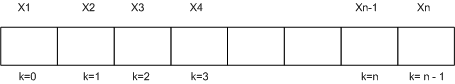
\includegraphics[width=.6\textwidth]{figs/fig_listas/lista-linear}
%%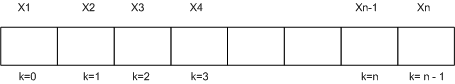
\includegraphics[height=0.50\paperheight, width=0.5\paperwidth]{figs/fig_listas/lista-linear}
	\end{figure} 

\begin{figure}[!hb]
	\centering
		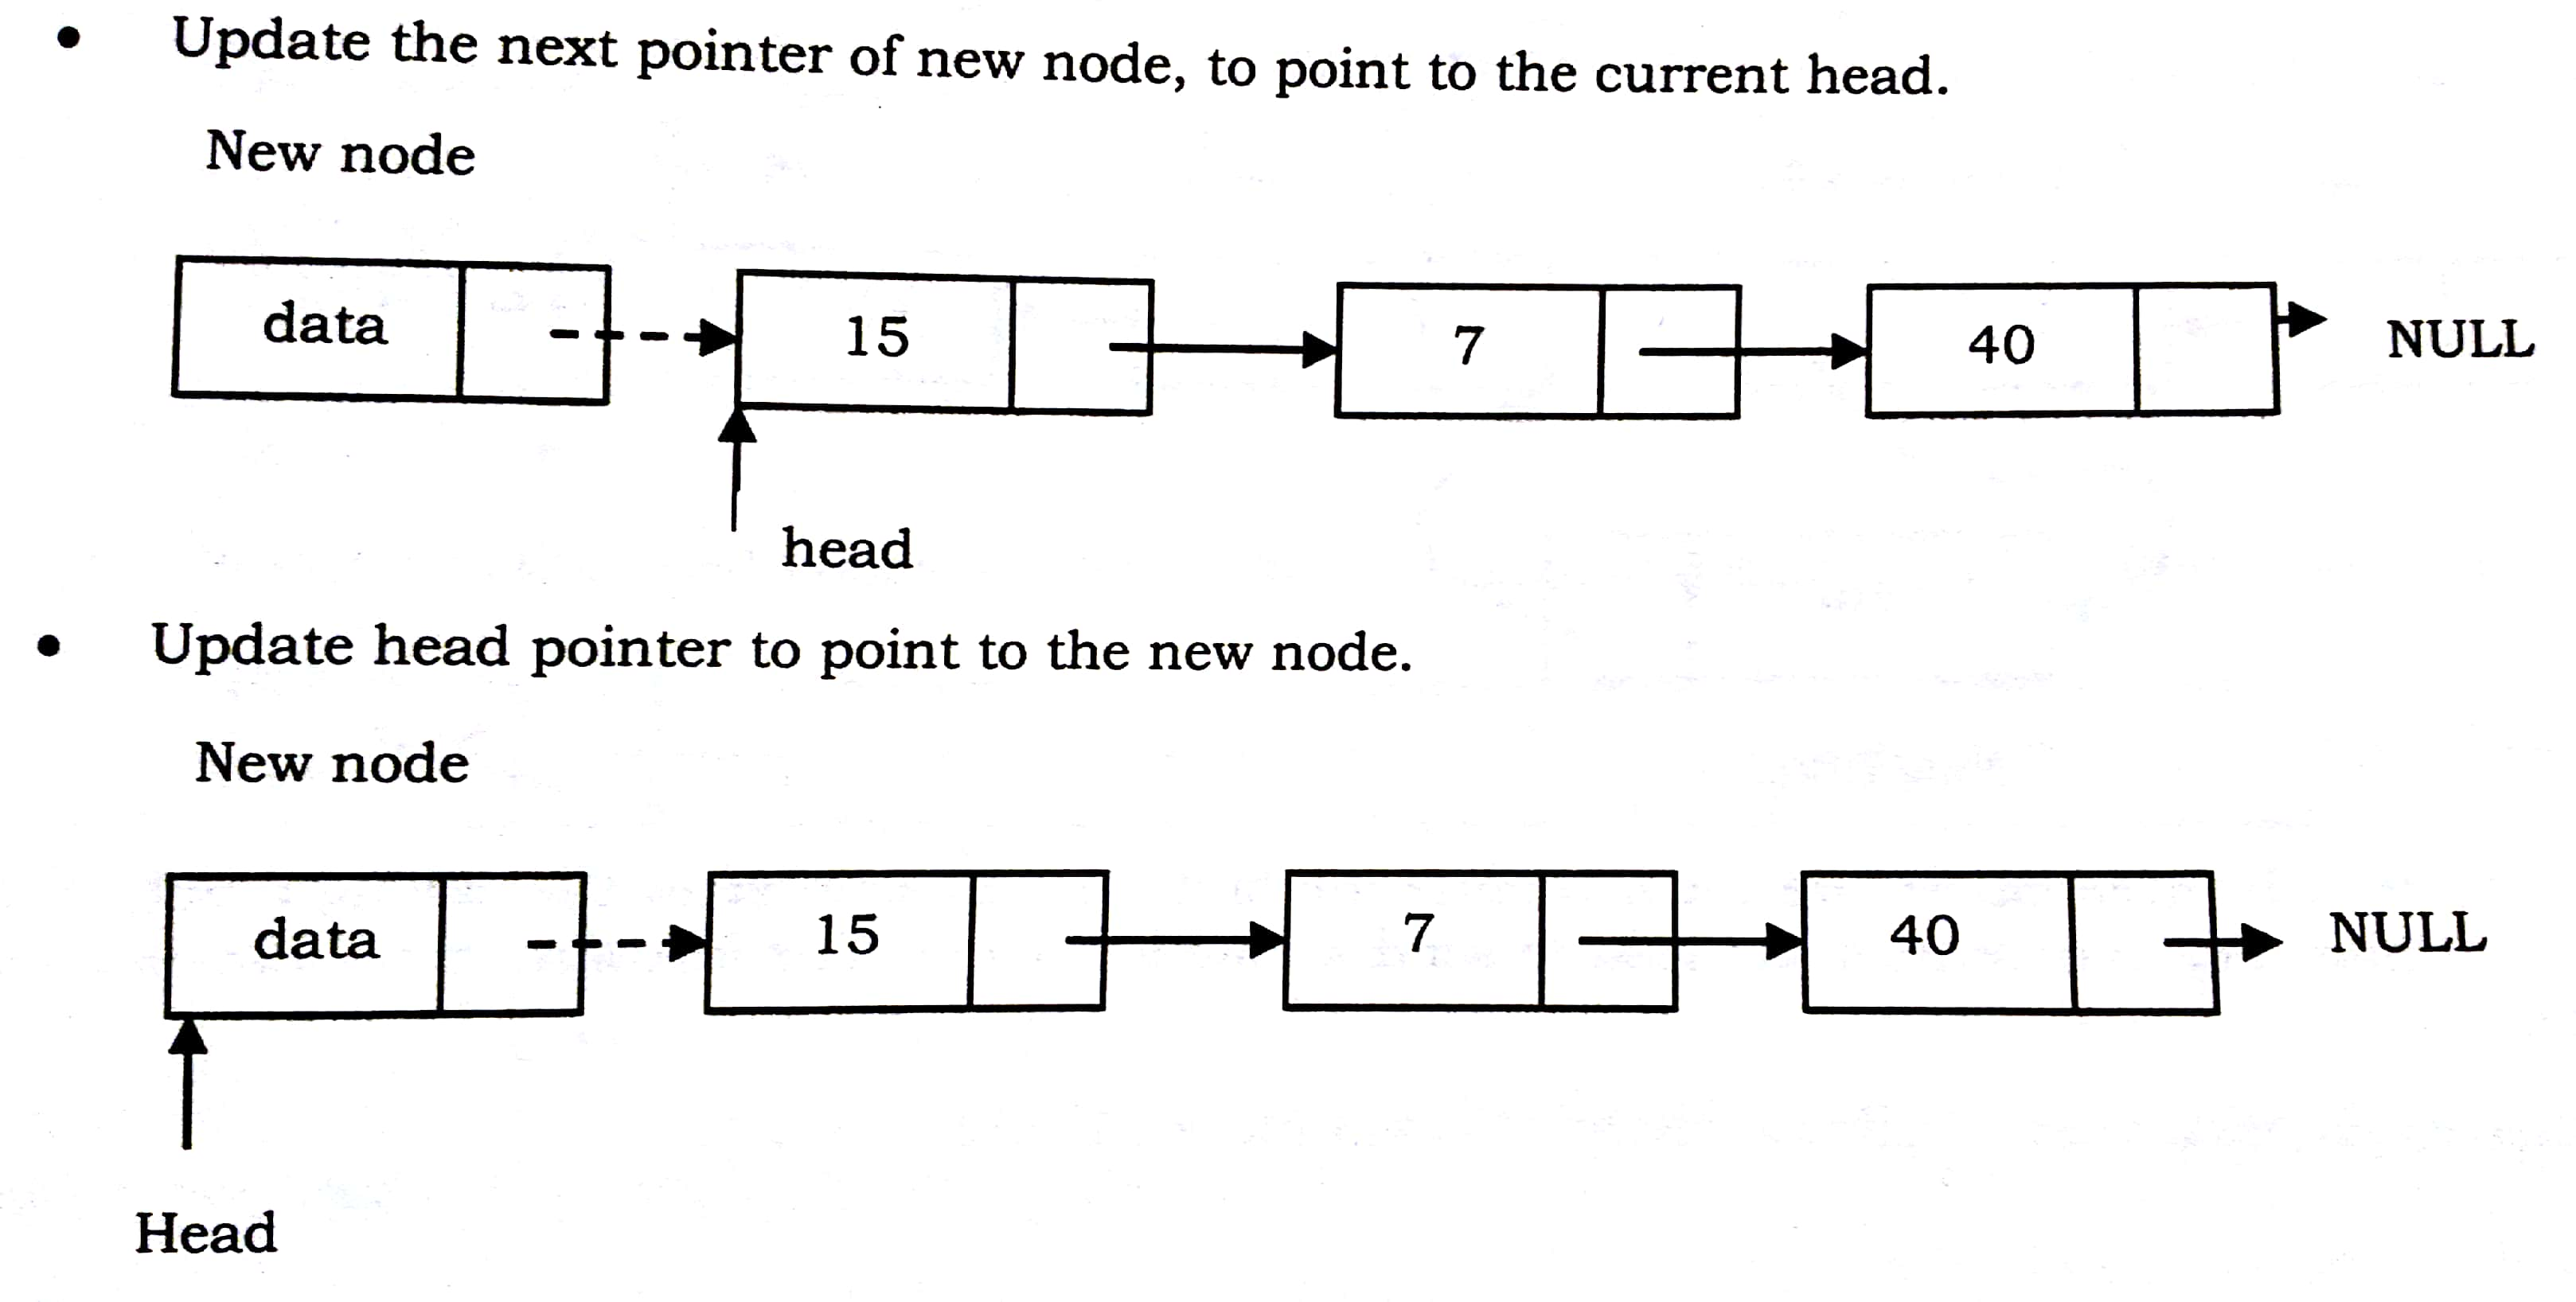
\includegraphics[height=0.50\paperheight, width=0.5\paperwidth]{figs/fig_listas/insere_inicio}			
			\caption{Incluir um nó no início da lista}	
%%				\label{fig:lista-linear-repre}
			\end{figure} 


\end{frame} 
%----------------------------------------------------------------------------------------------------------
%[allowframebreaks=0.9]

\begin{frame}%%%[allowframebreaks=0.98]

\frametitle{Incluindo um nó numa posição da  lista}

\begin{figure}[!hb]
	\centering
%%		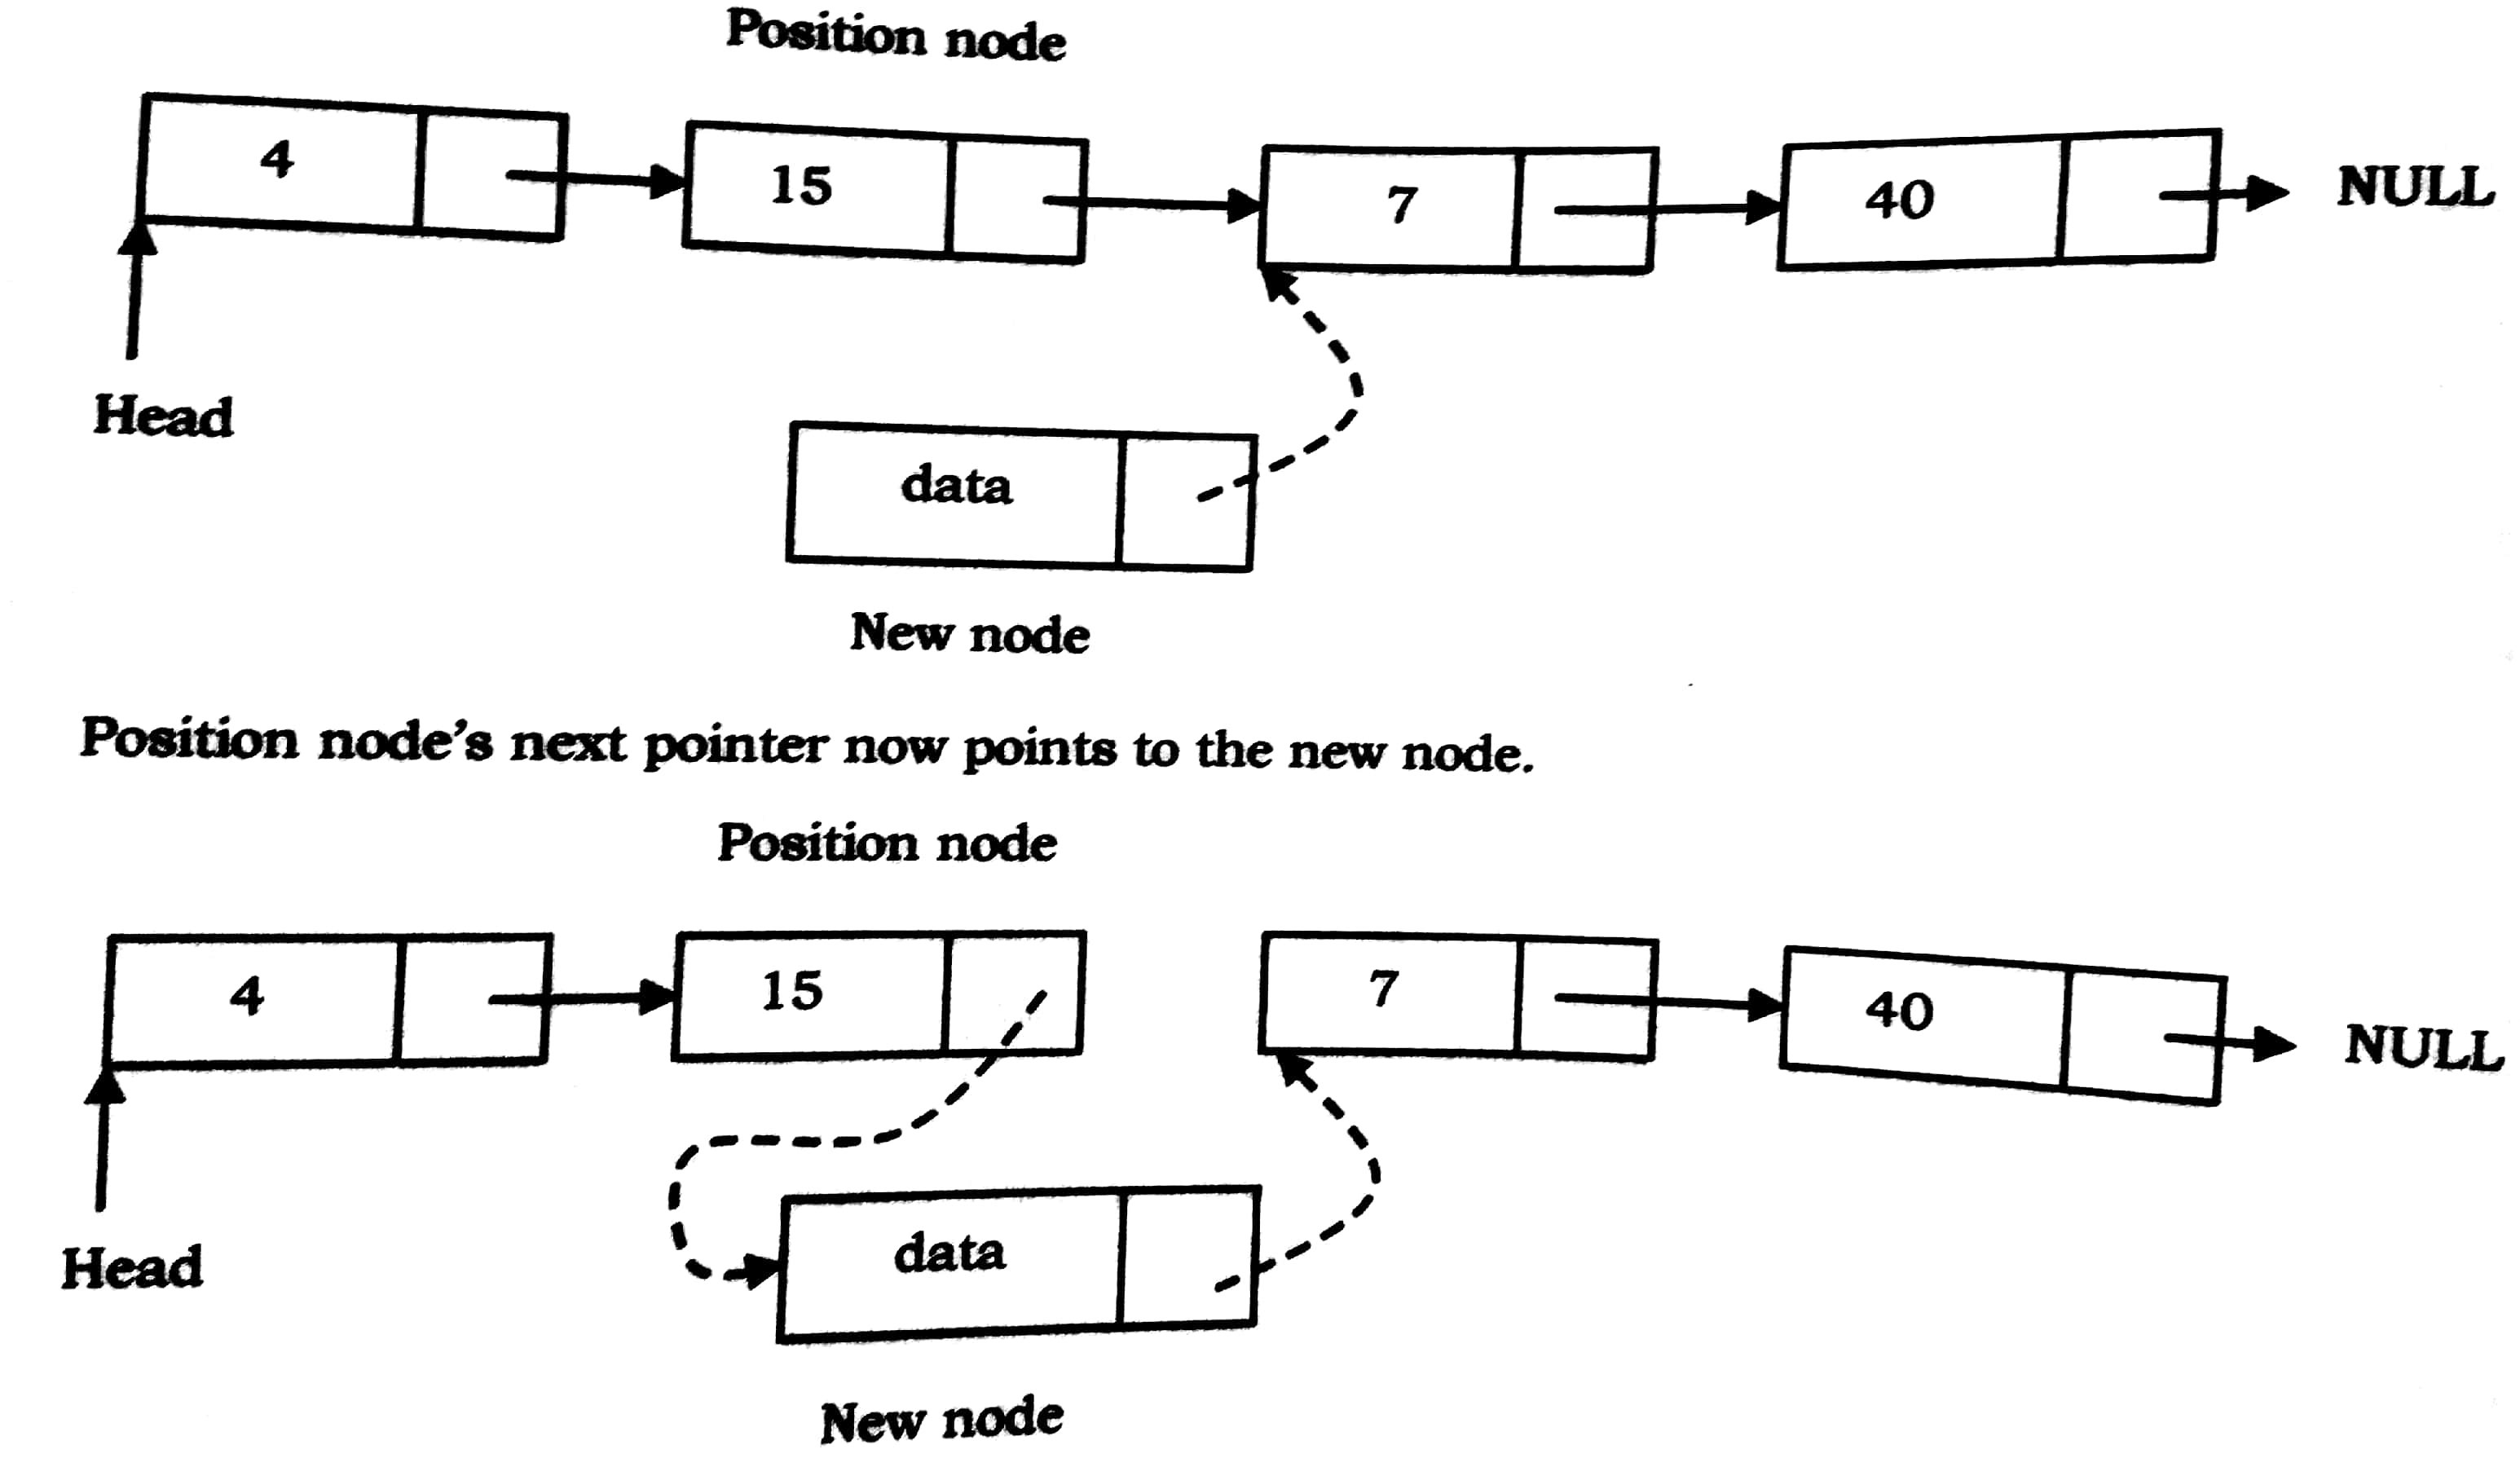
\includegraphics[scale=0.1]{figs/fig_listas/insere_posicao}
	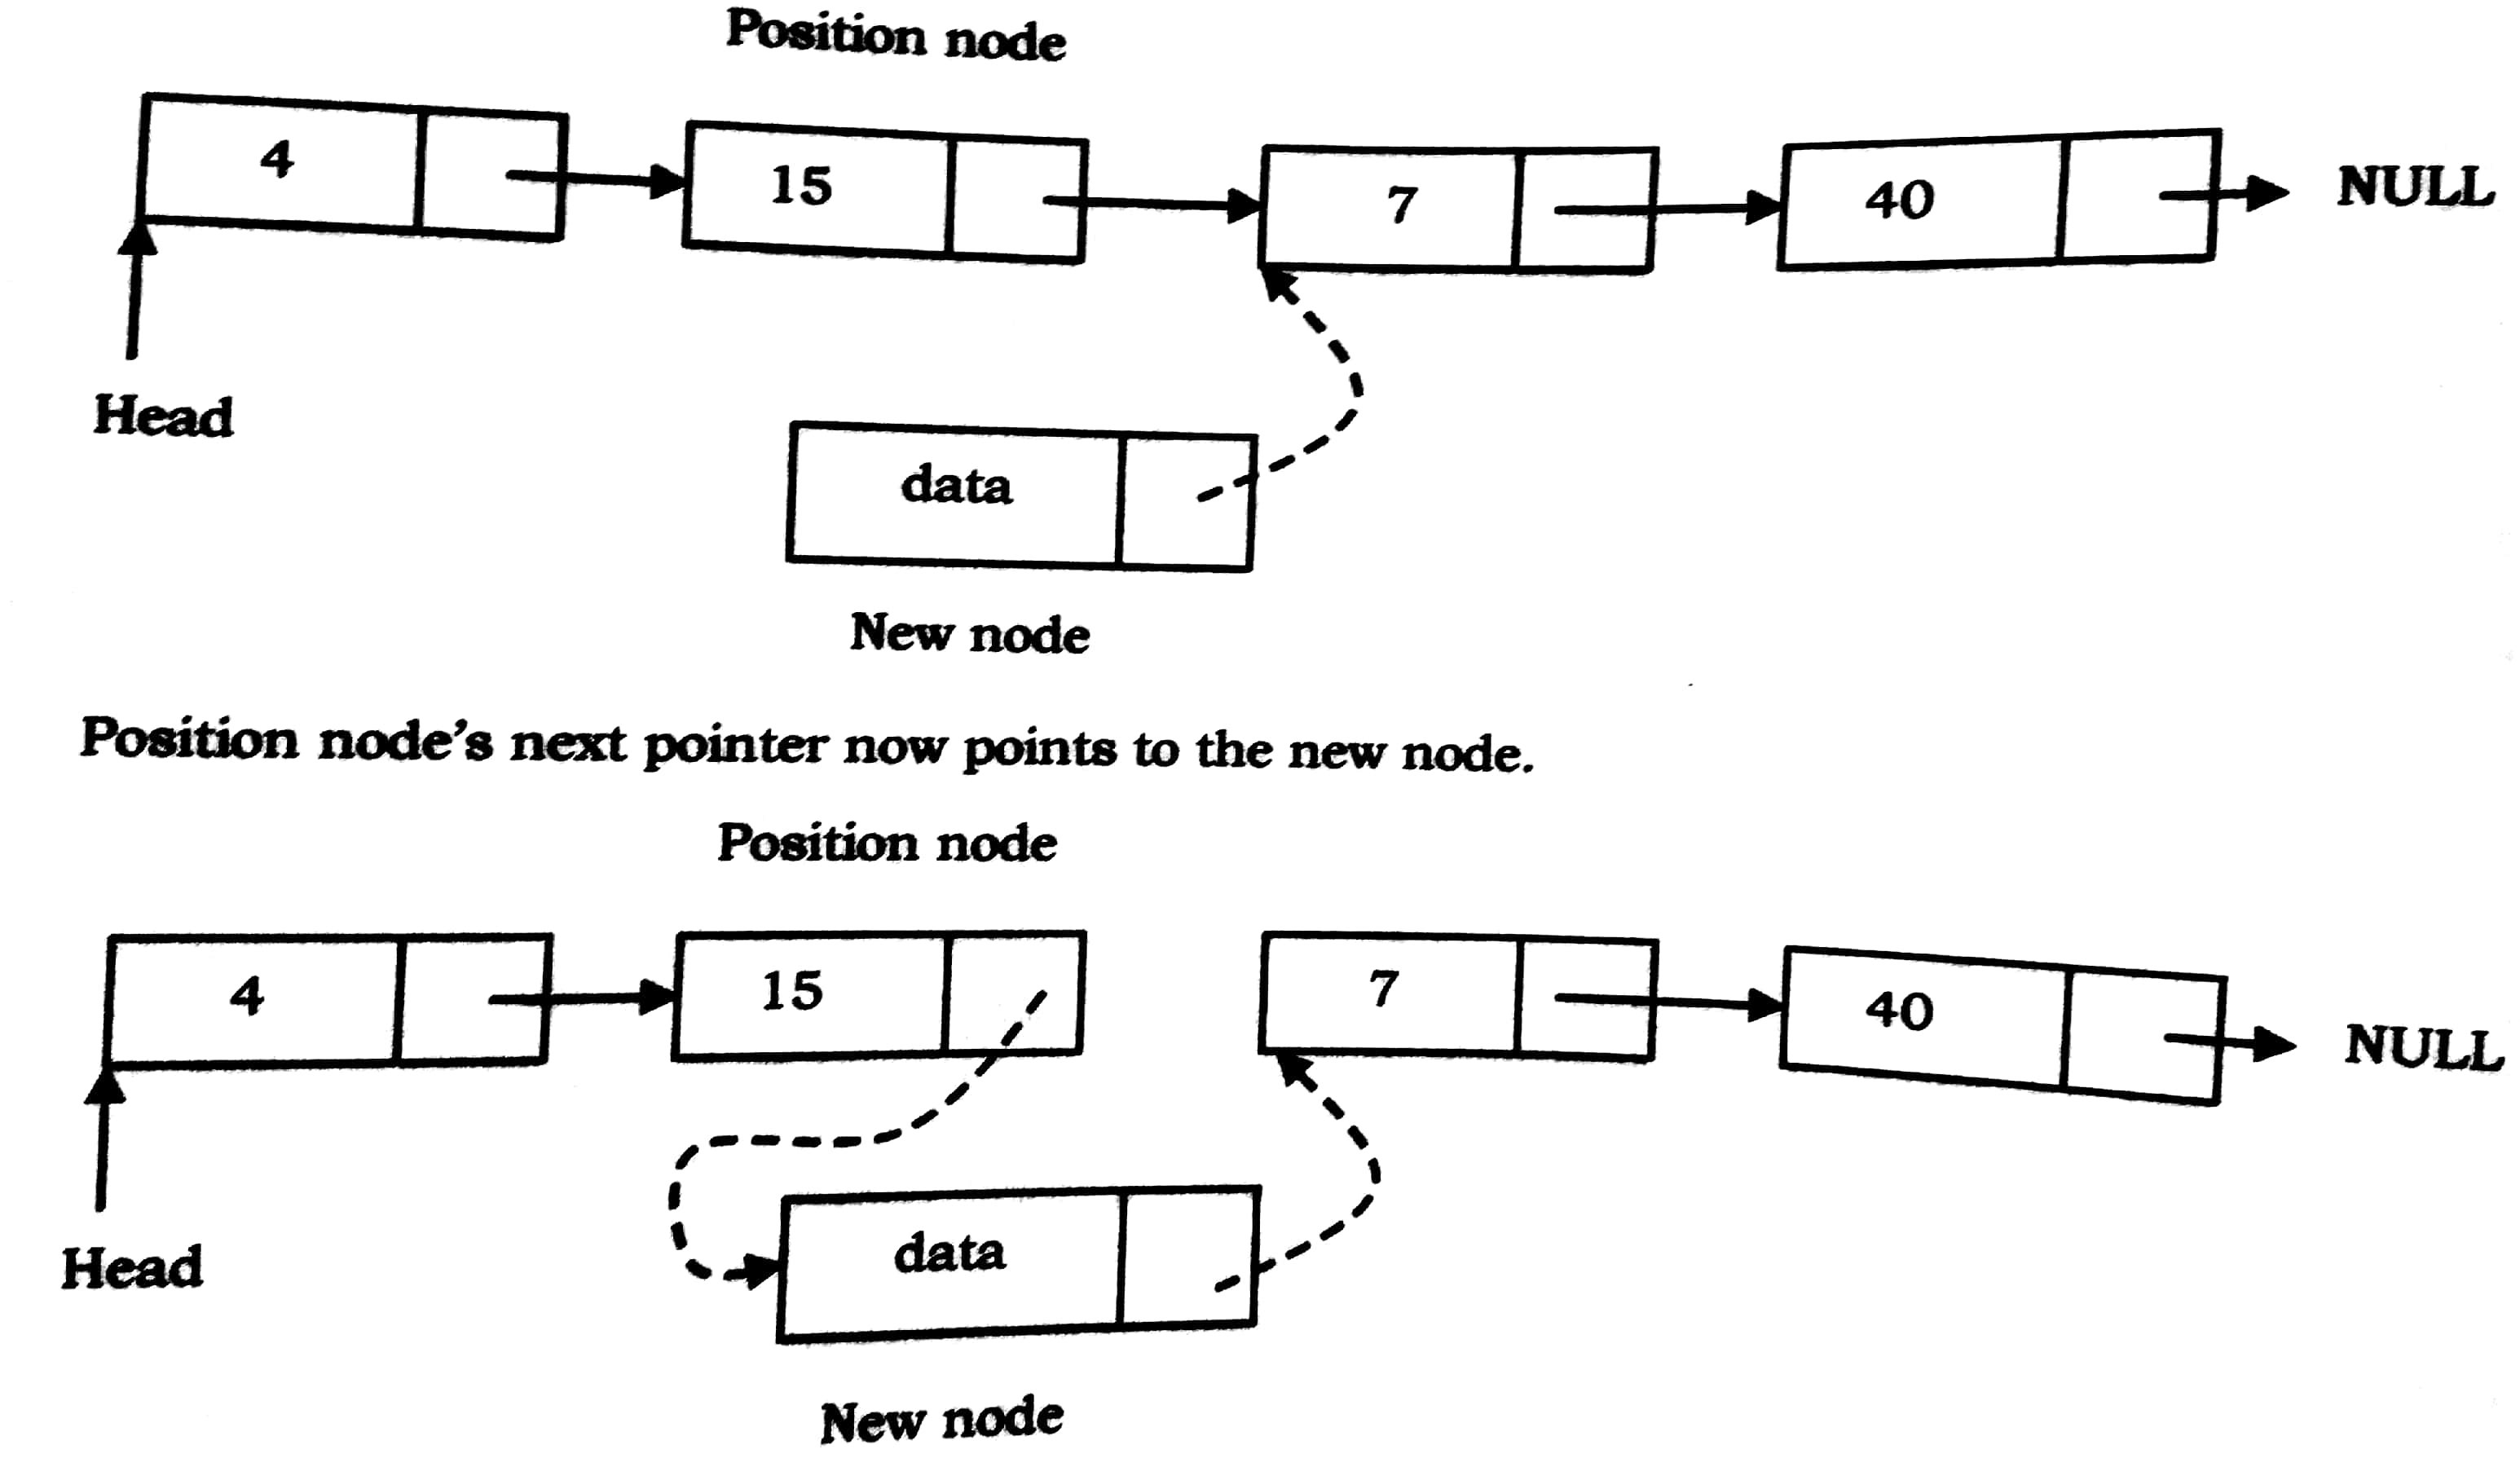
\includegraphics[height=0.50\paperheight, width=0.7\paperwidth]{figs/fig_listas/insere_posicao}						
			\caption{Incluir um nó numa posição da lista}	
%%				\label{fig:lista-linear-repre}
		\end{figure} 

\end{frame} 
%----------------------------------------------------------------------------------------------------------
%[allowframebreaks=0.9]

\begin{frame}%%%[allowframebreaks=0.98]

\frametitle{Excluindo o nó no início da lista -- \textit{cabeça} da lista}

\begin{figure}[!hb]
	\centering
%%		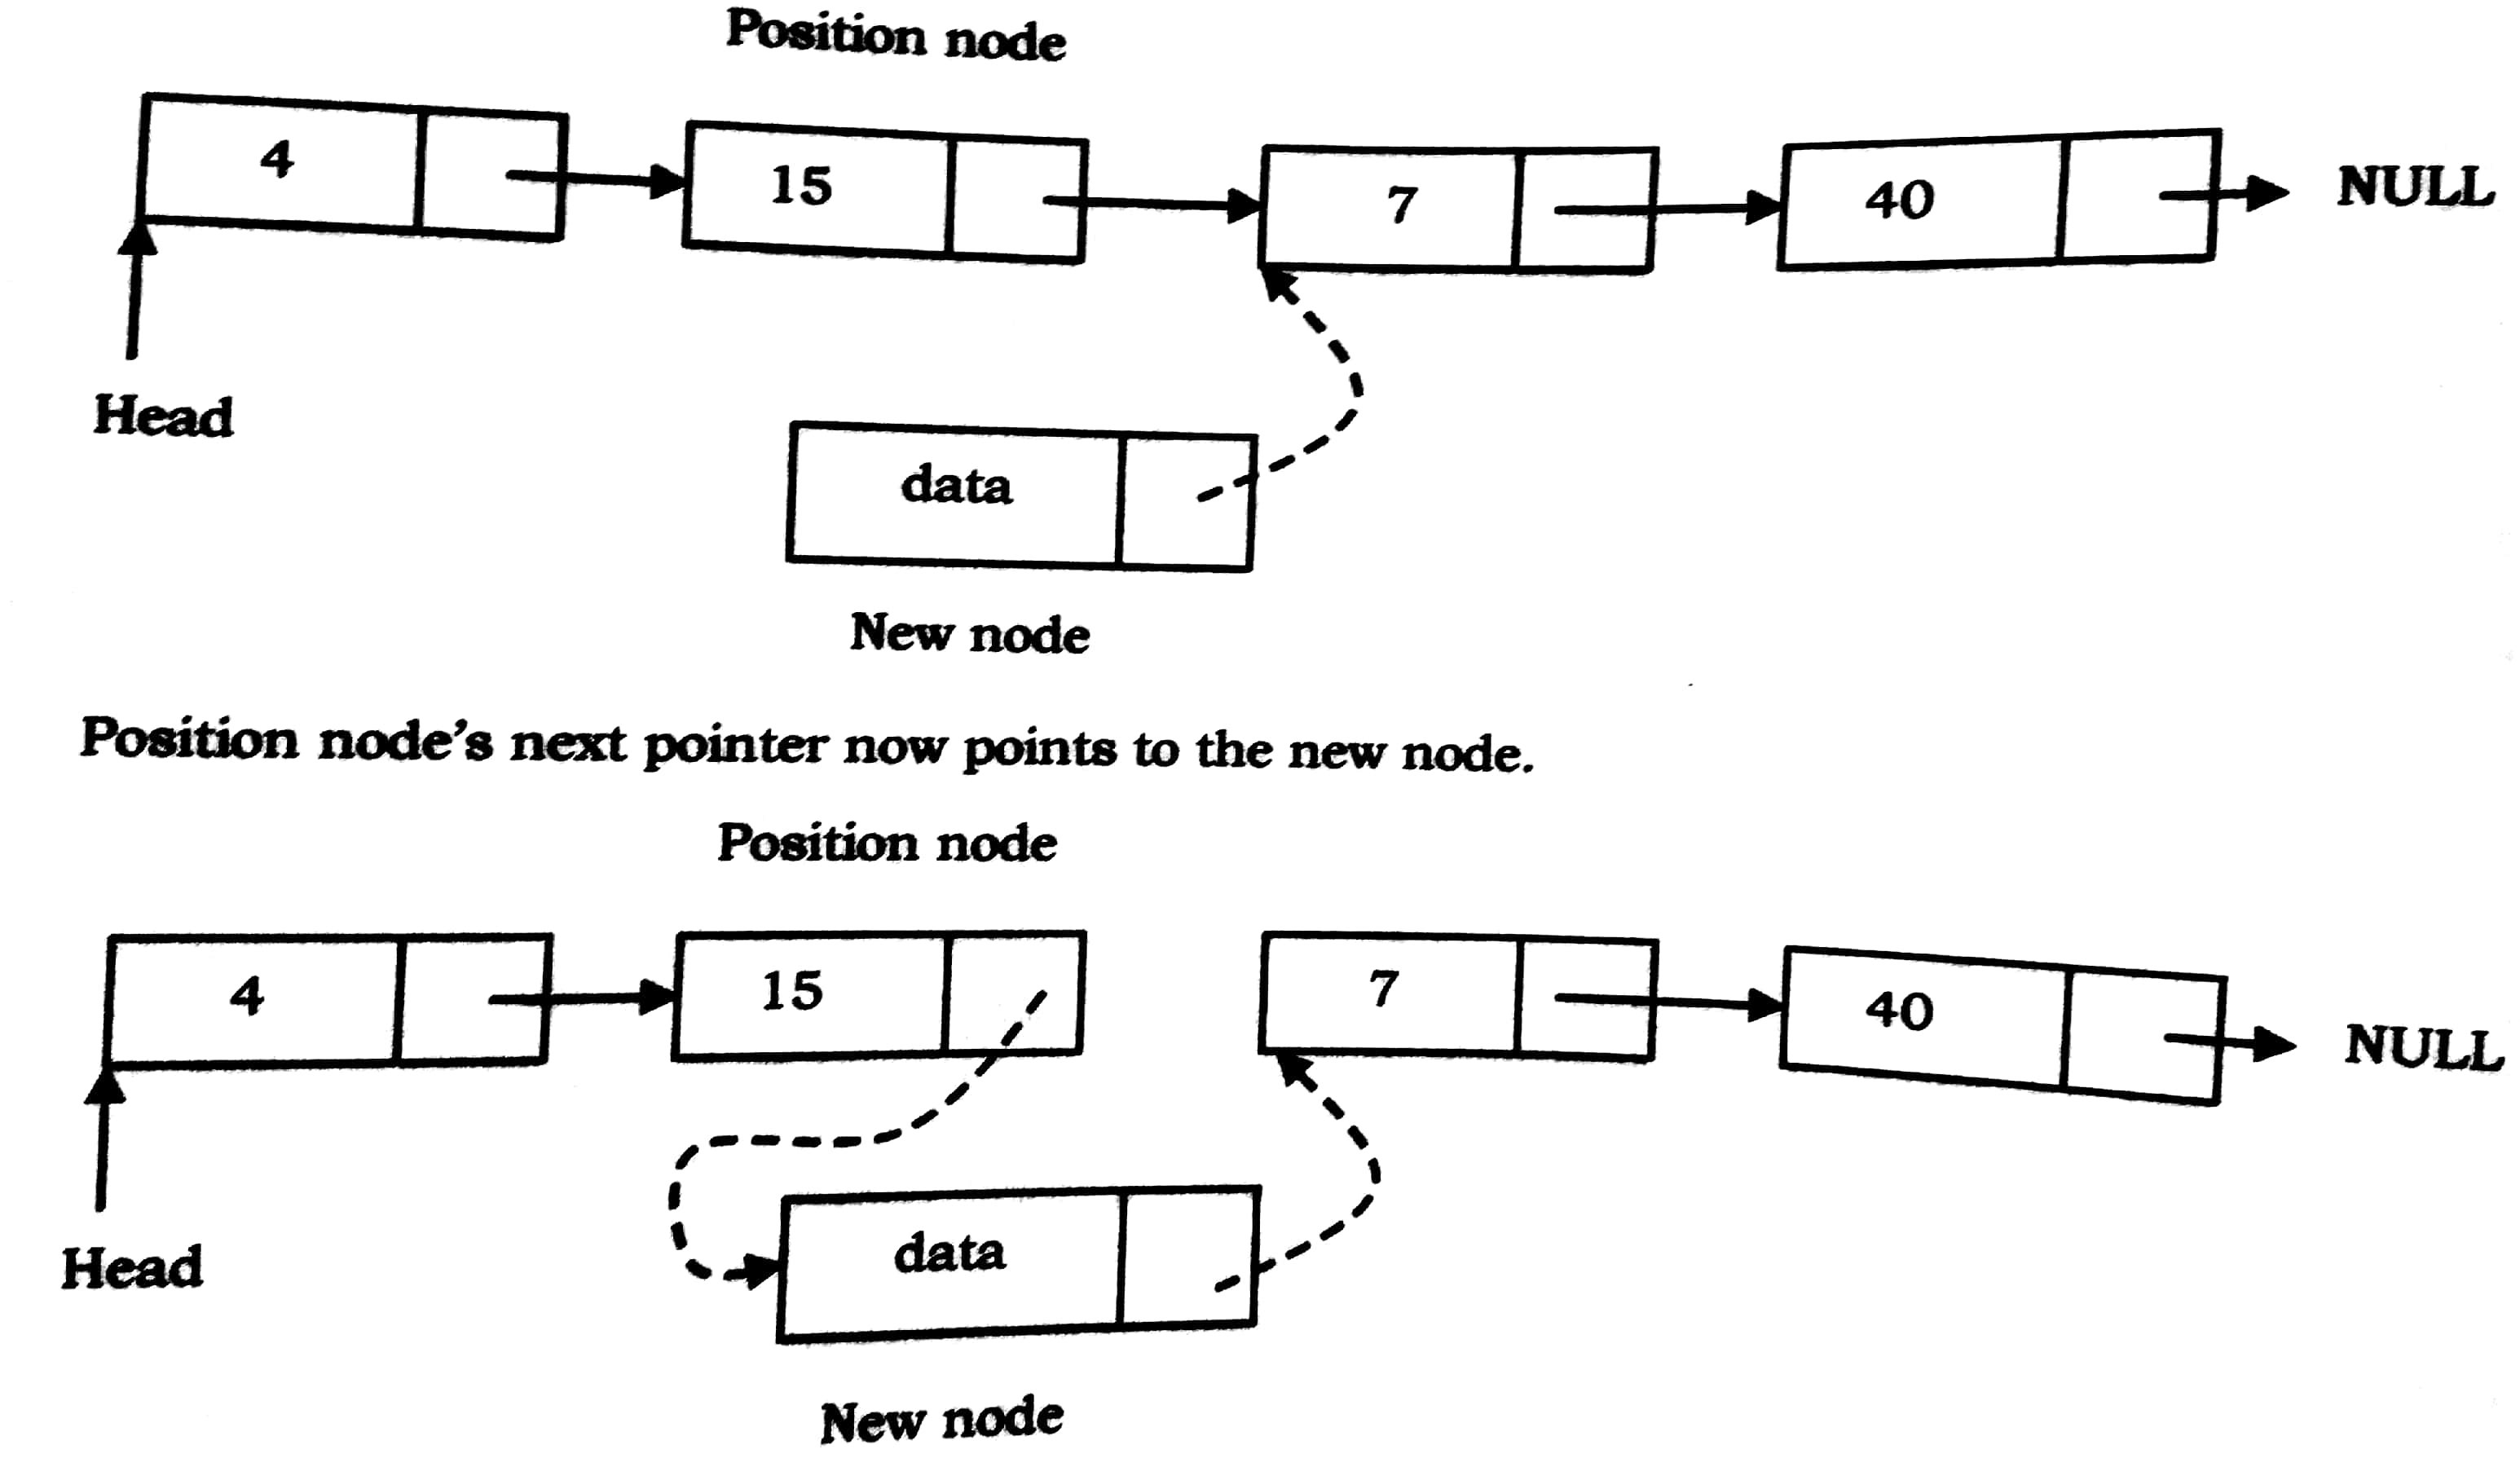
\includegraphics[scale=0.1]{figs/fig_listas/insere_posicao}
	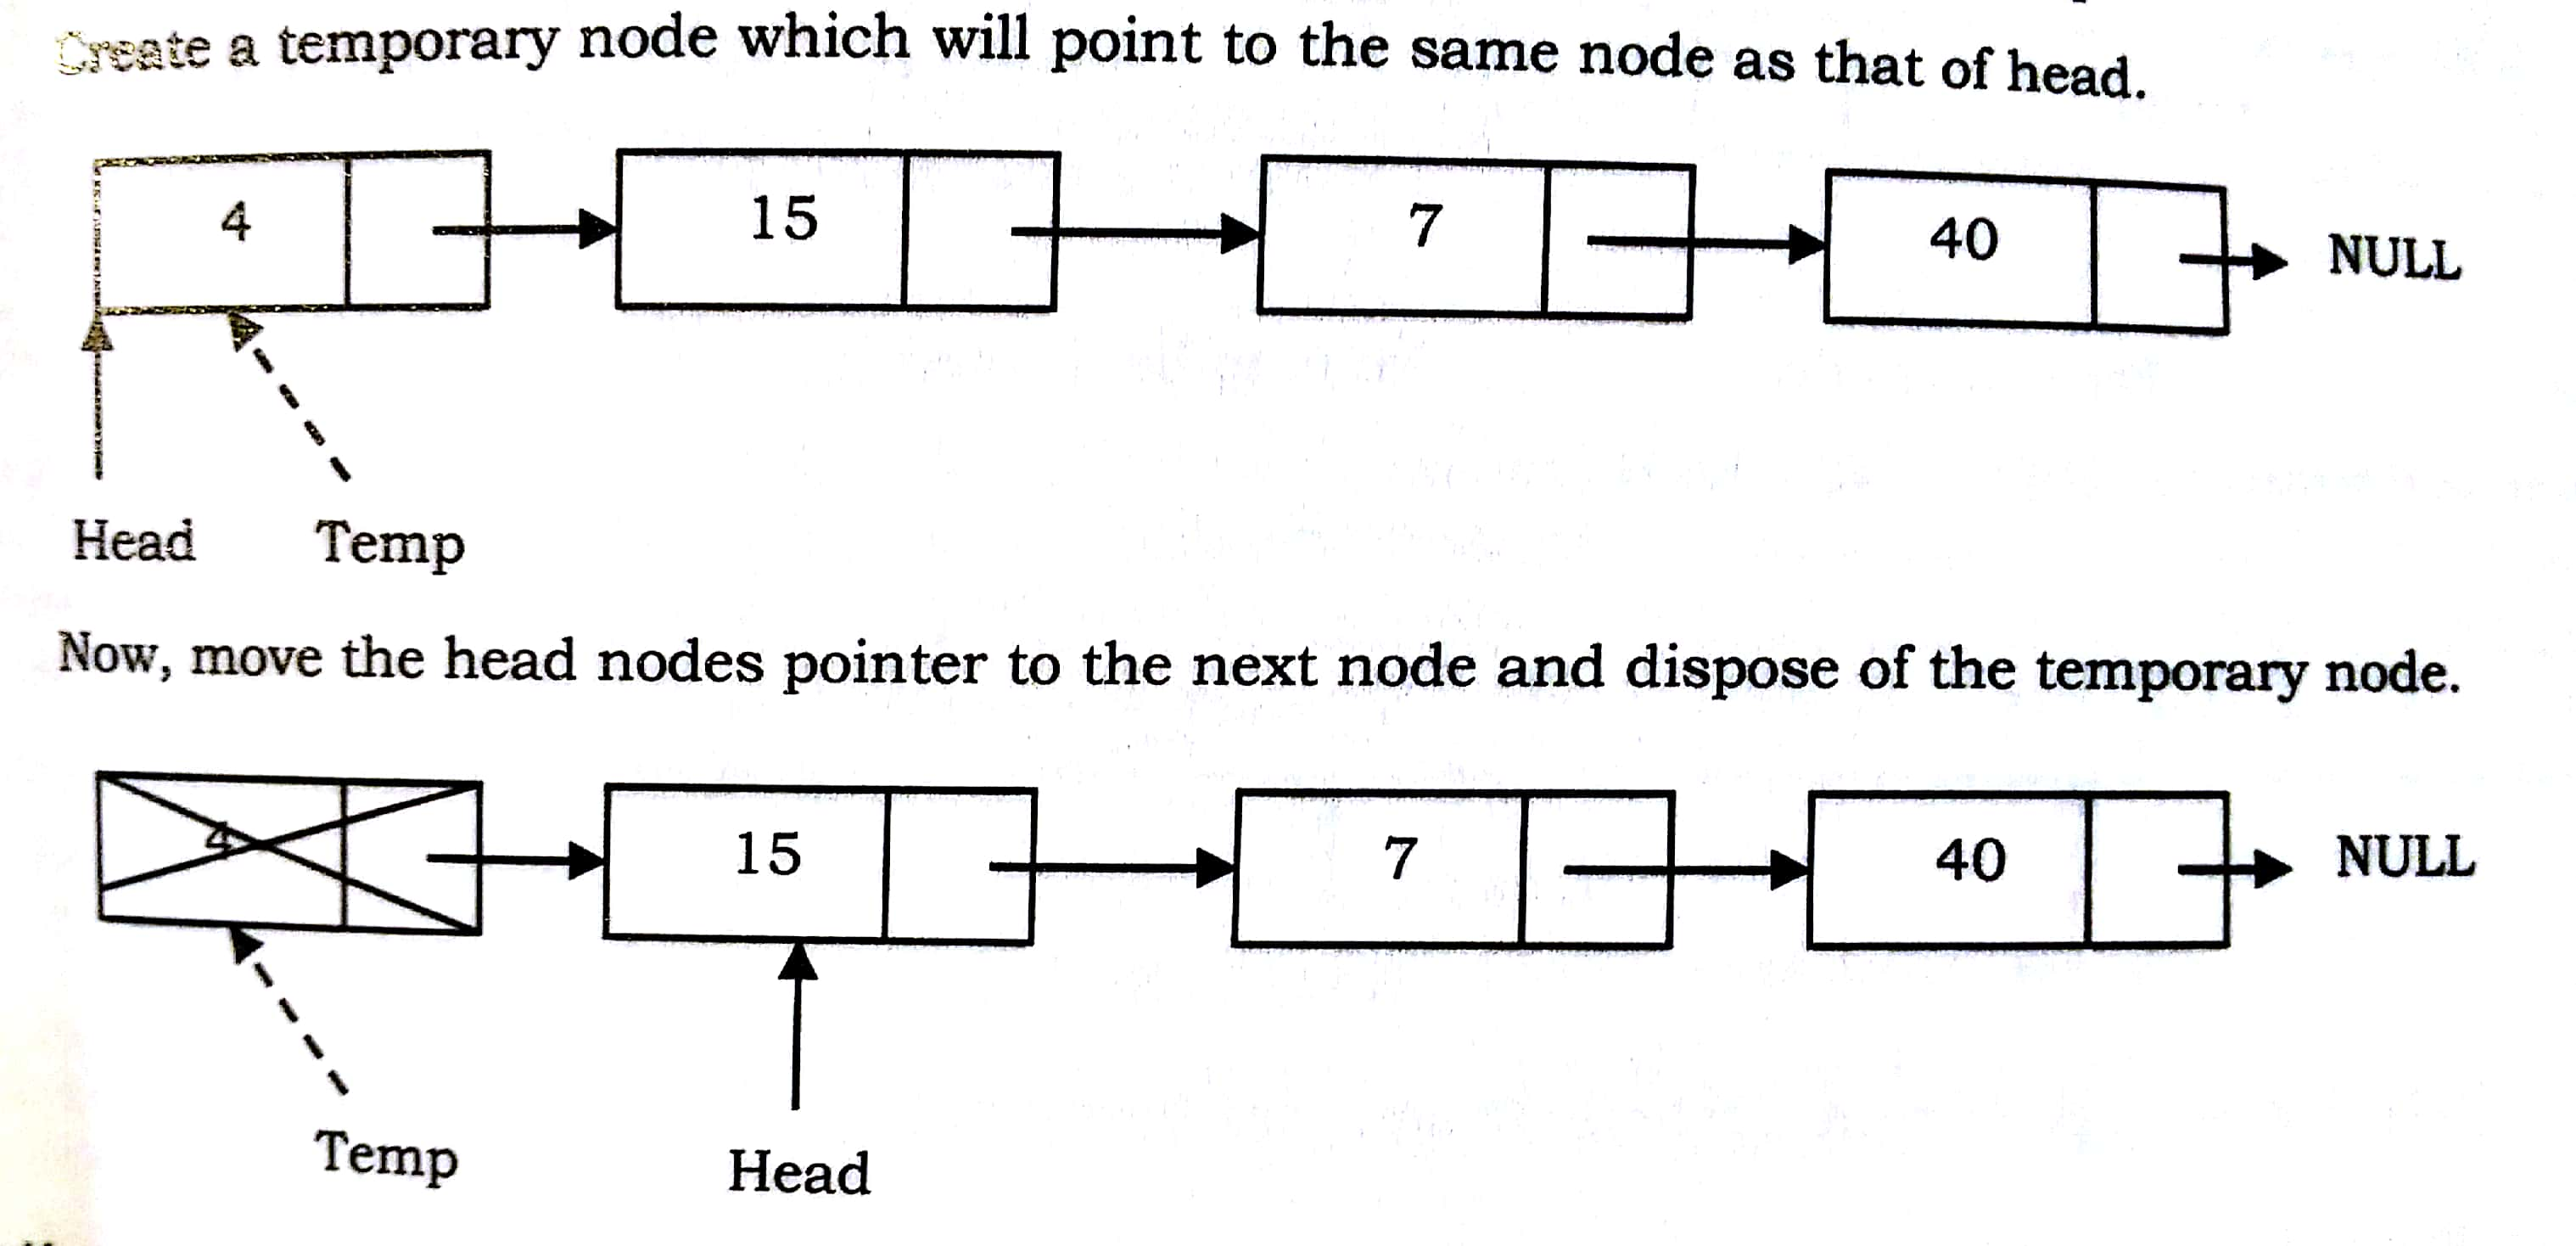
\includegraphics[height=0.50\paperheight, width=0.7\paperwidth]{figs/fig_listas/exclui_inicio}						
			\caption{Exclui o nó no início da lista}	
%%				\label{fig:lista-linear-repre}
		\end{figure} 

\end{frame} 

%----------------------------------------------------------------------------------------------------------

\begin{frame}%%%[allowframebreaks=0.98]

\frametitle{Excluindo um nó no  meio  da lista}

\begin{figure}[!hb]
	\centering
%%		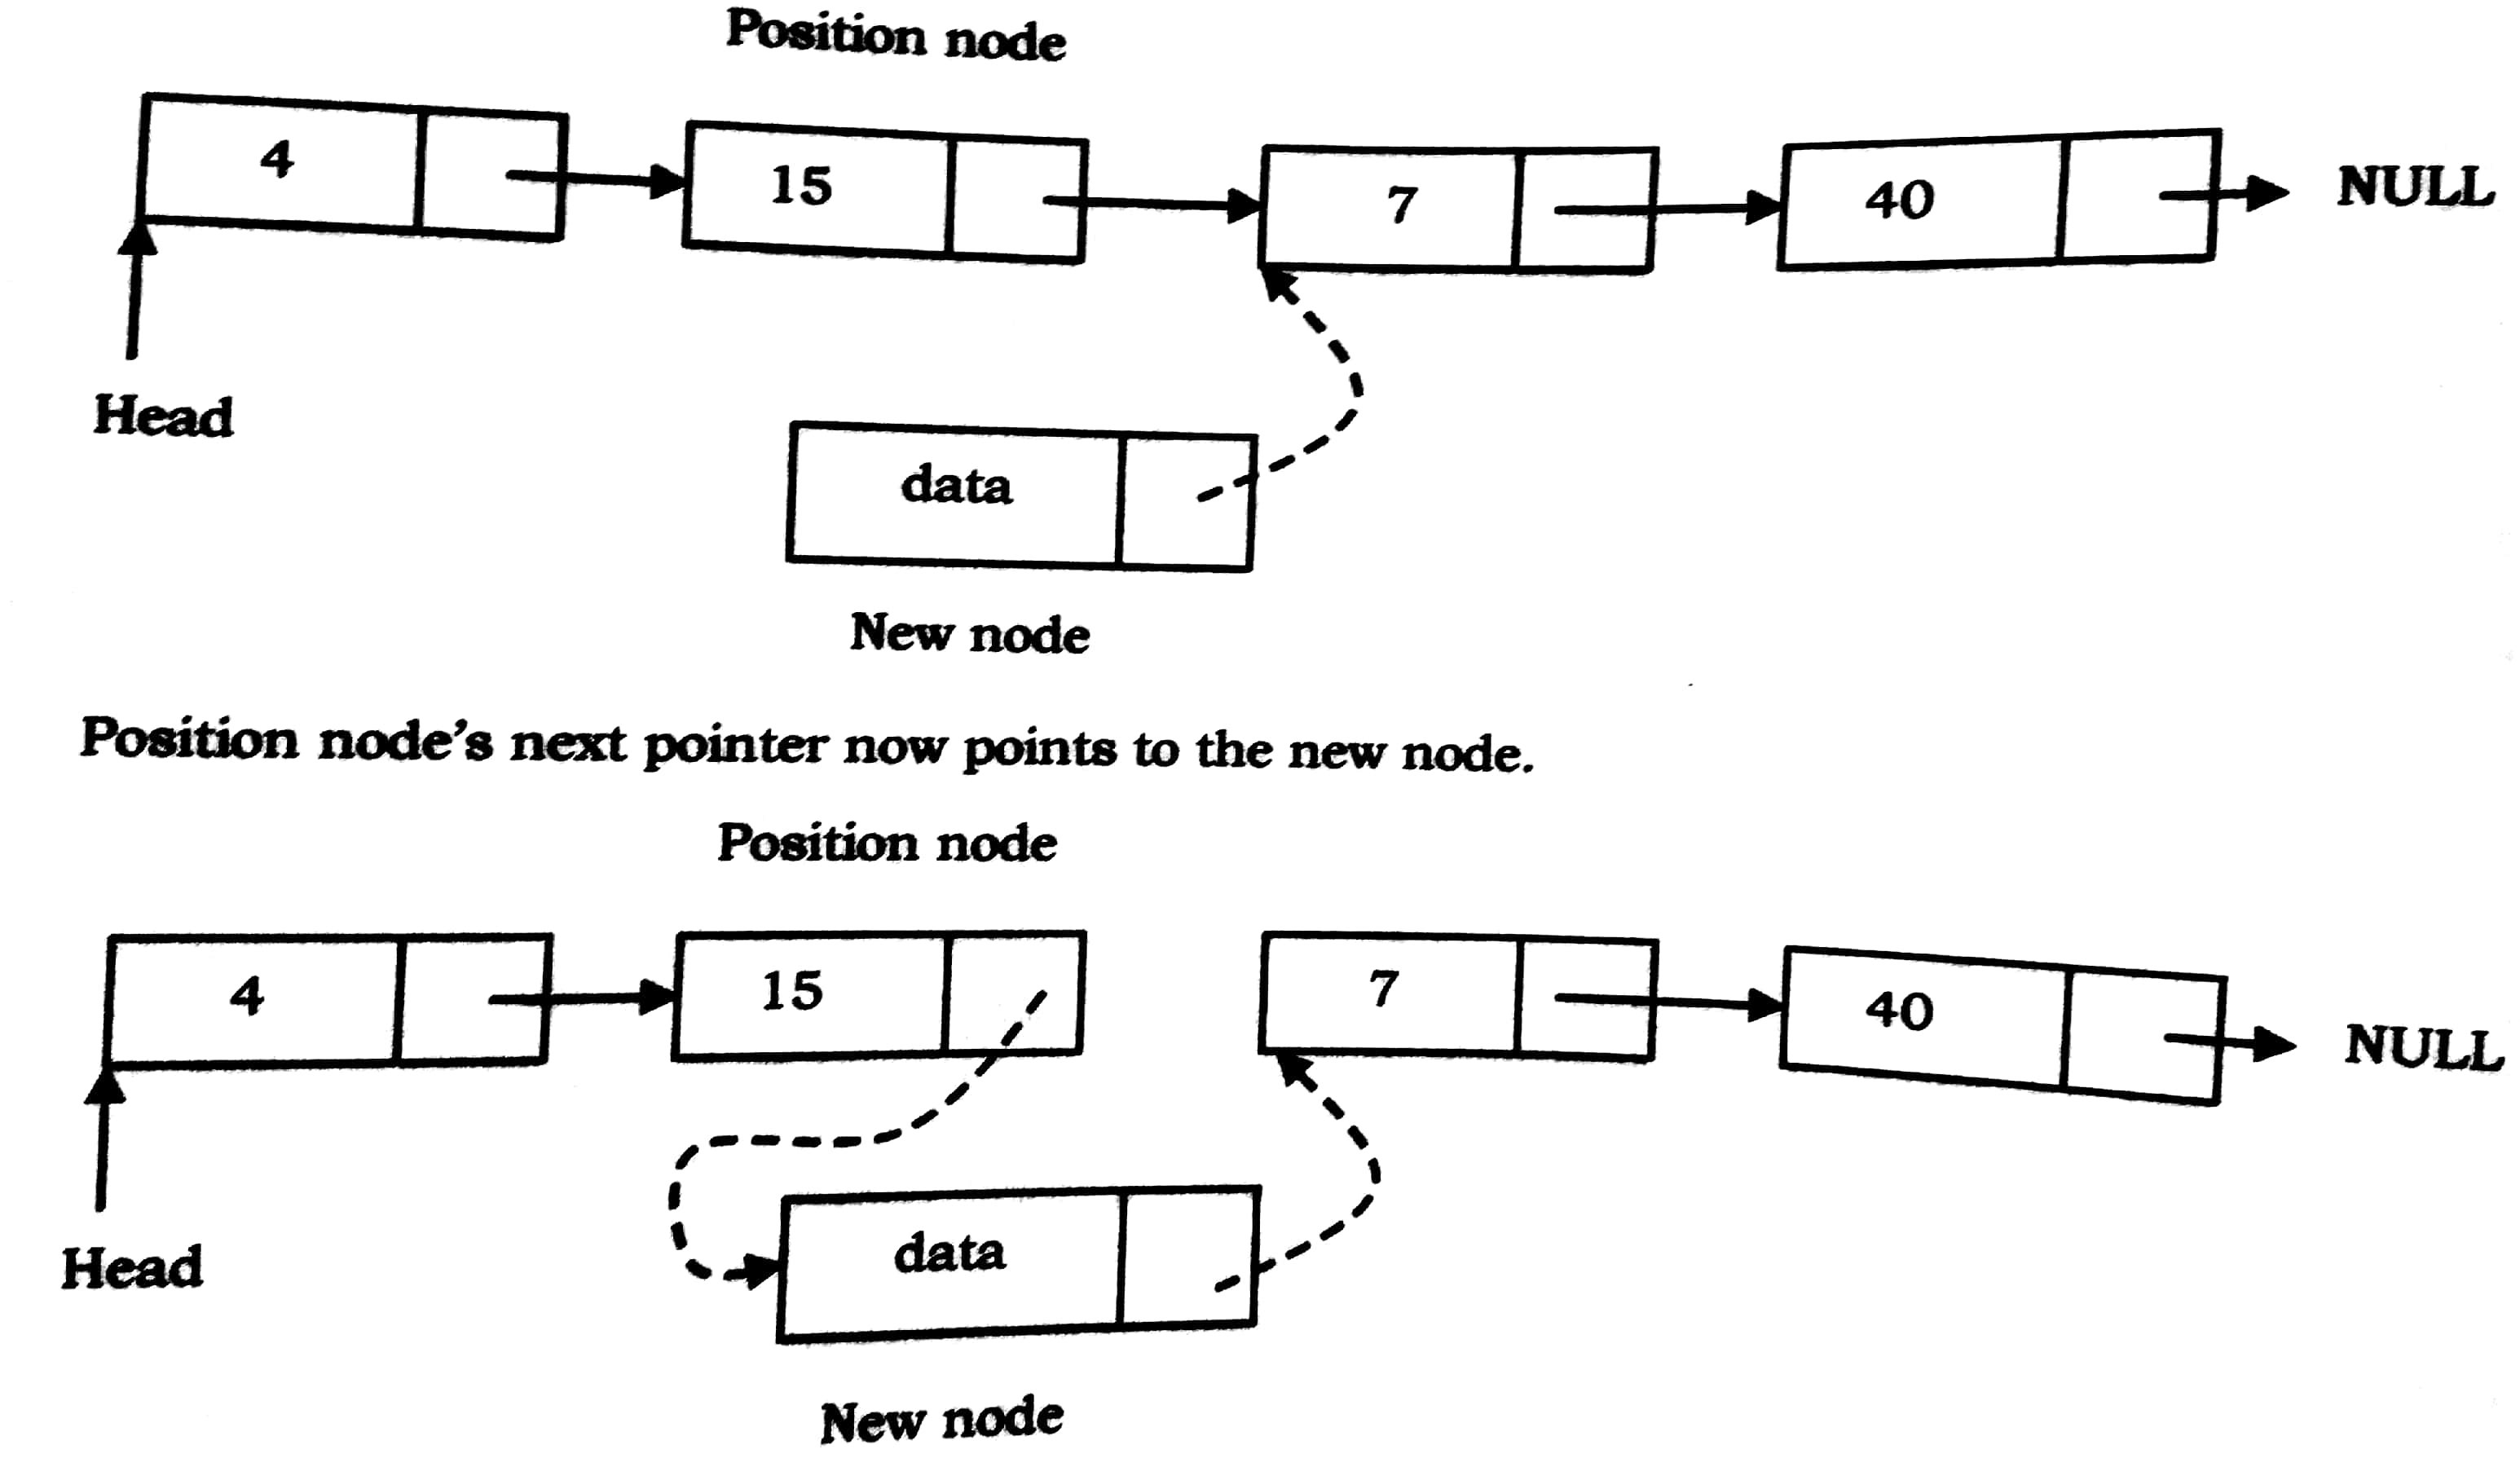
\includegraphics[scale=0.1]{figs/fig_listas/insere_posicao}
	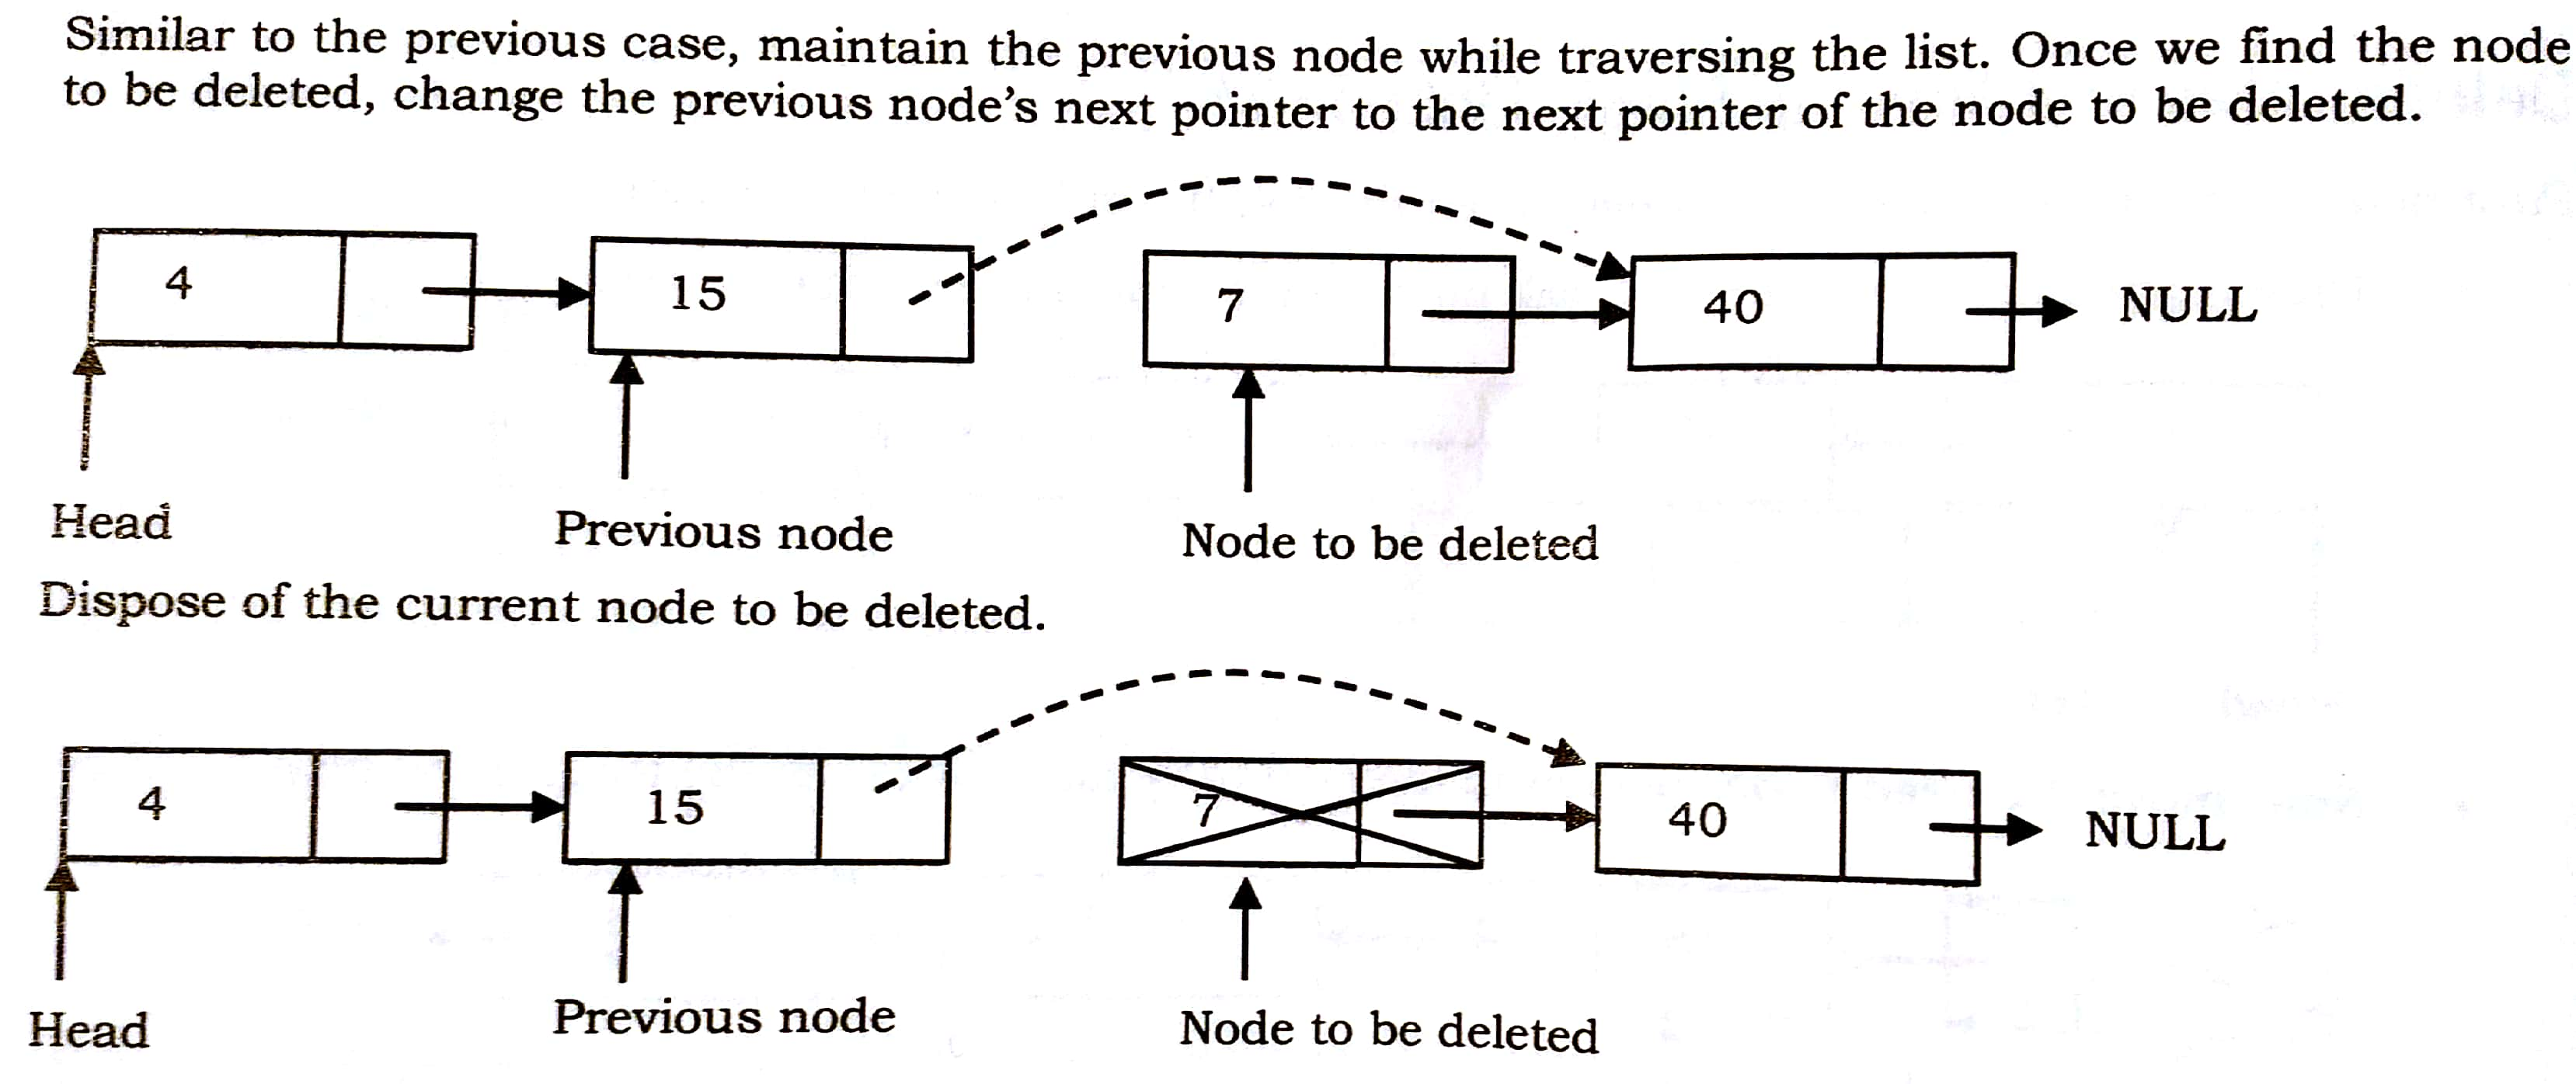
\includegraphics[height=0.50\paperheight, width=0.7\paperwidth]{figs/fig_listas/exclui_no_meio}						
			\caption{Exclui nó no  meio  da lista -- k-ésima posição ou por conteúdo}	
%%				\label{fig:lista-linear-repre}
		\end{figure} 

\end{frame} 

%----------------------------------------------------------------------------------------------------------

\begin{frame}%%%[allowframebreaks=0.98]

\frametitle{Excluindo o último nó da lista}

\begin{figure}[!hb]
	\centering
%%		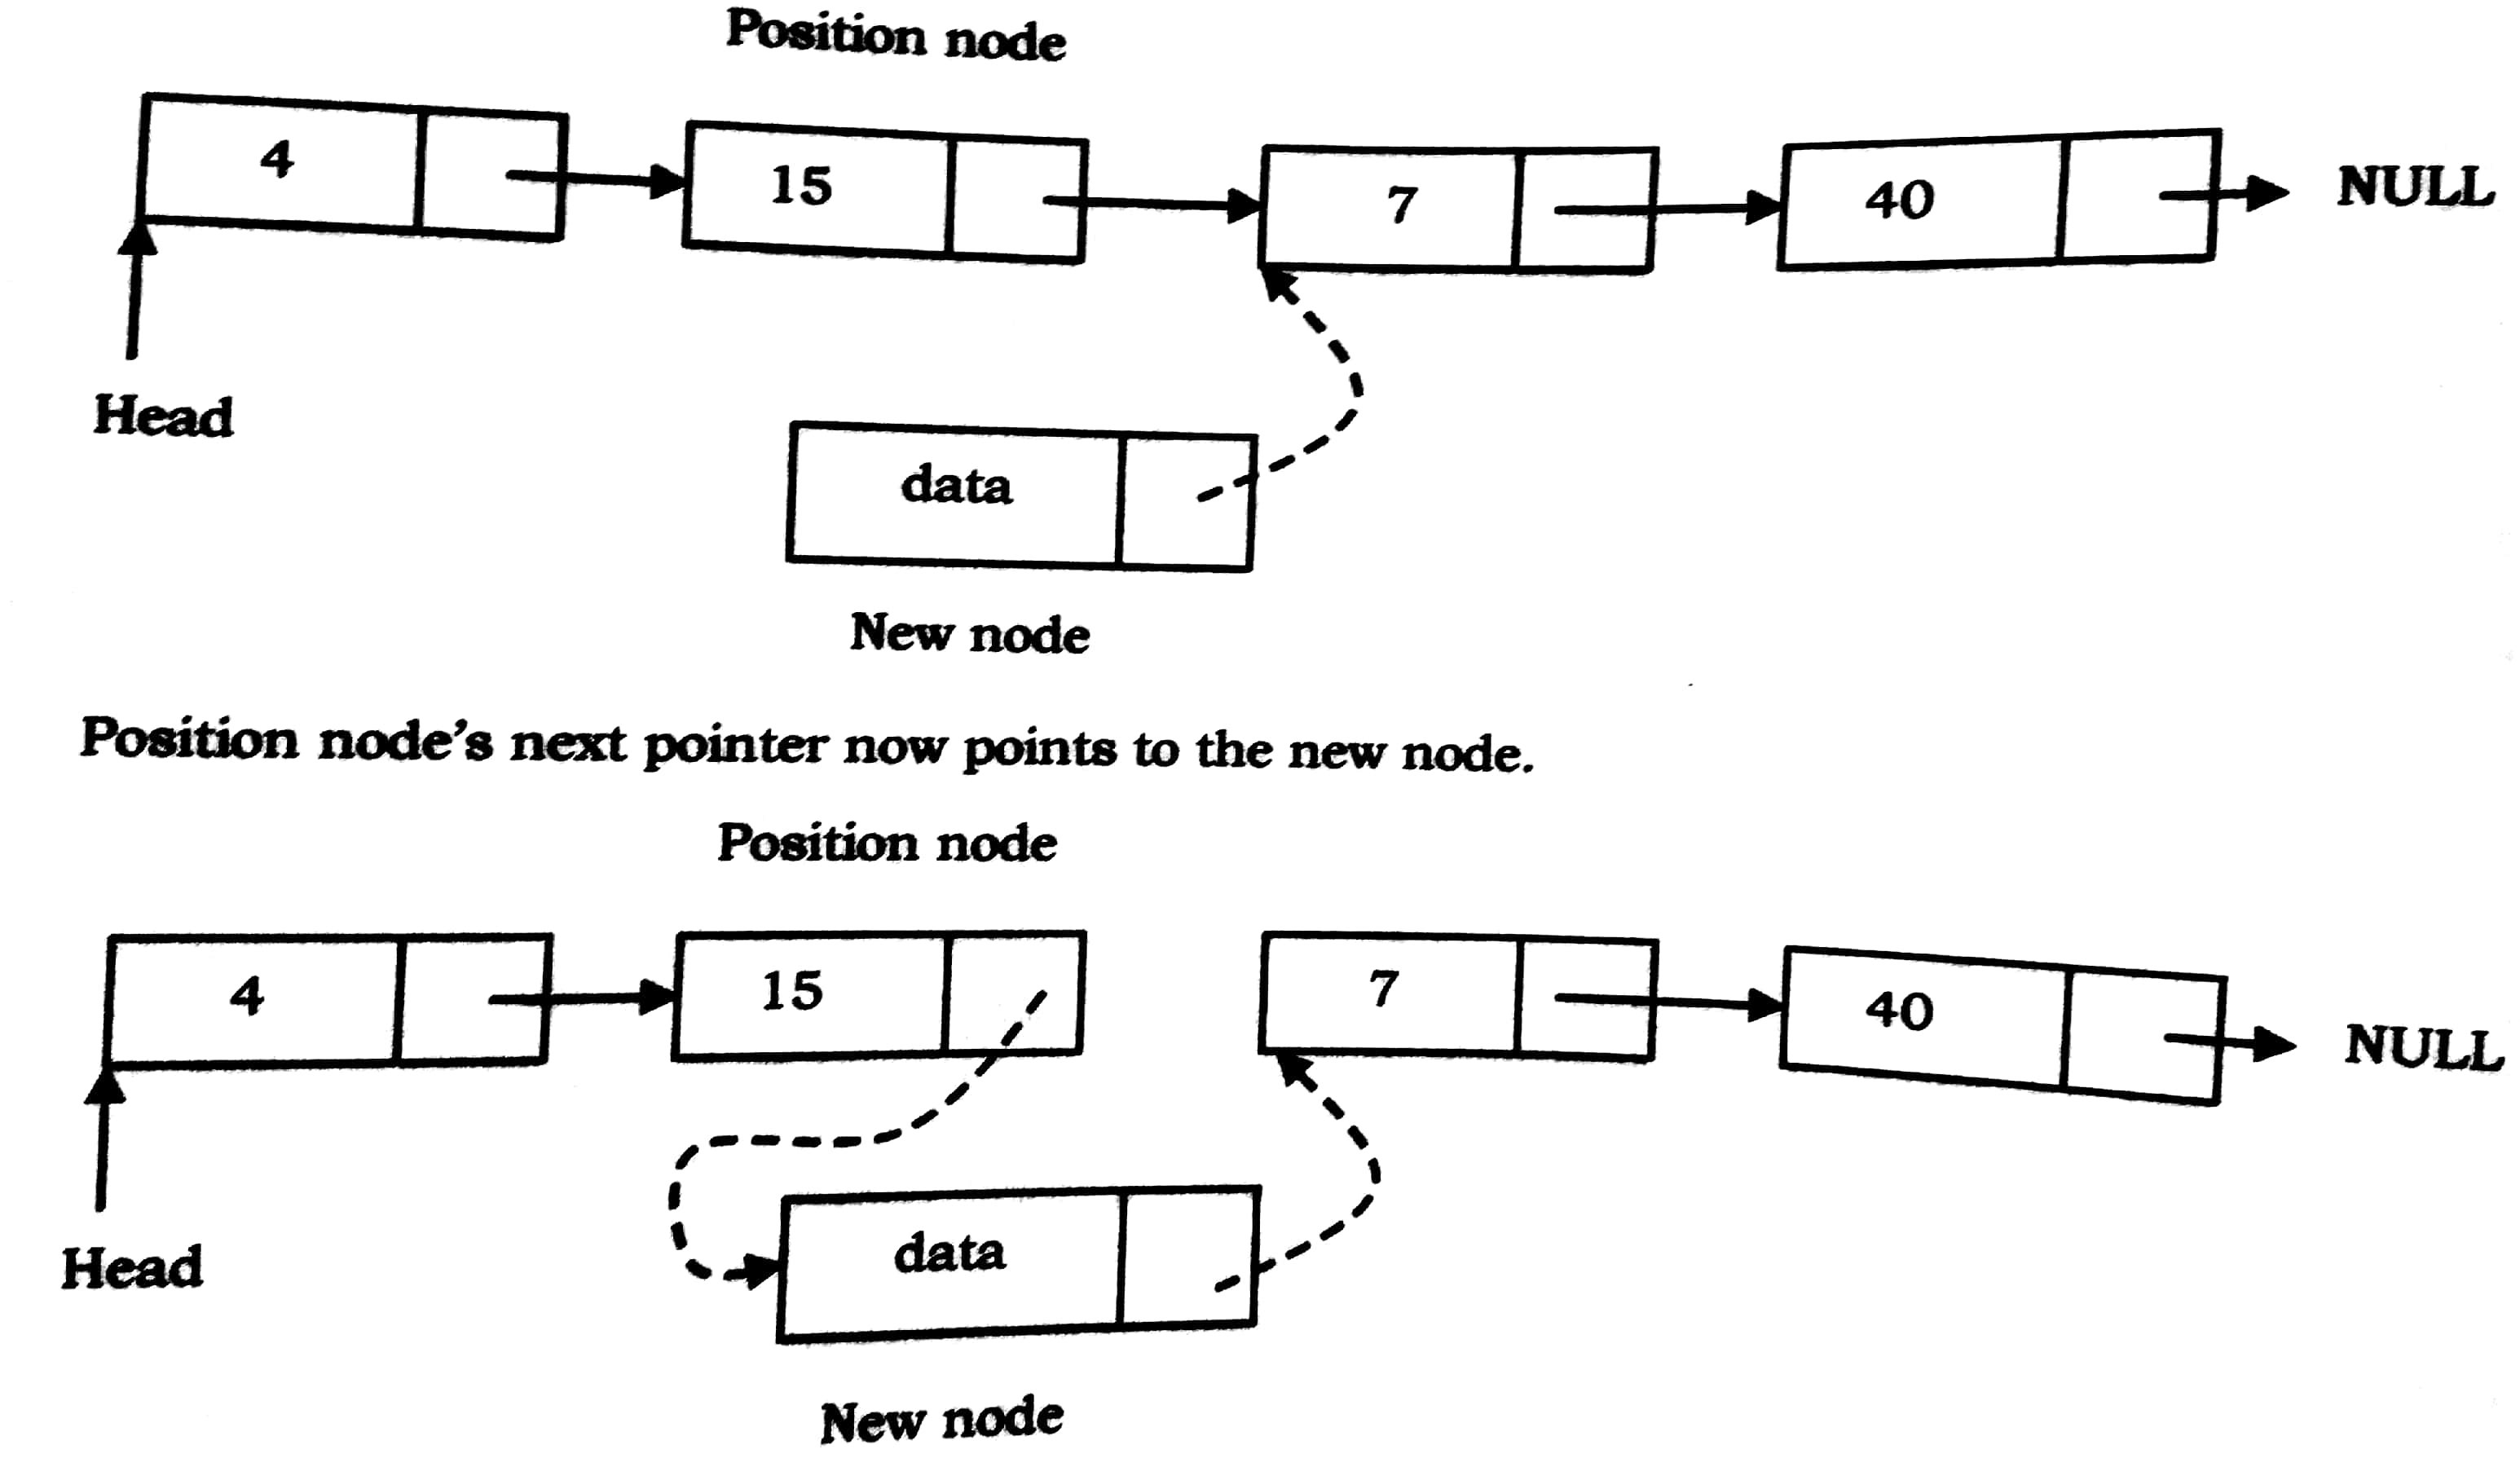
\includegraphics[scale=0.1]{figs/fig_listas/insere_posicao}
	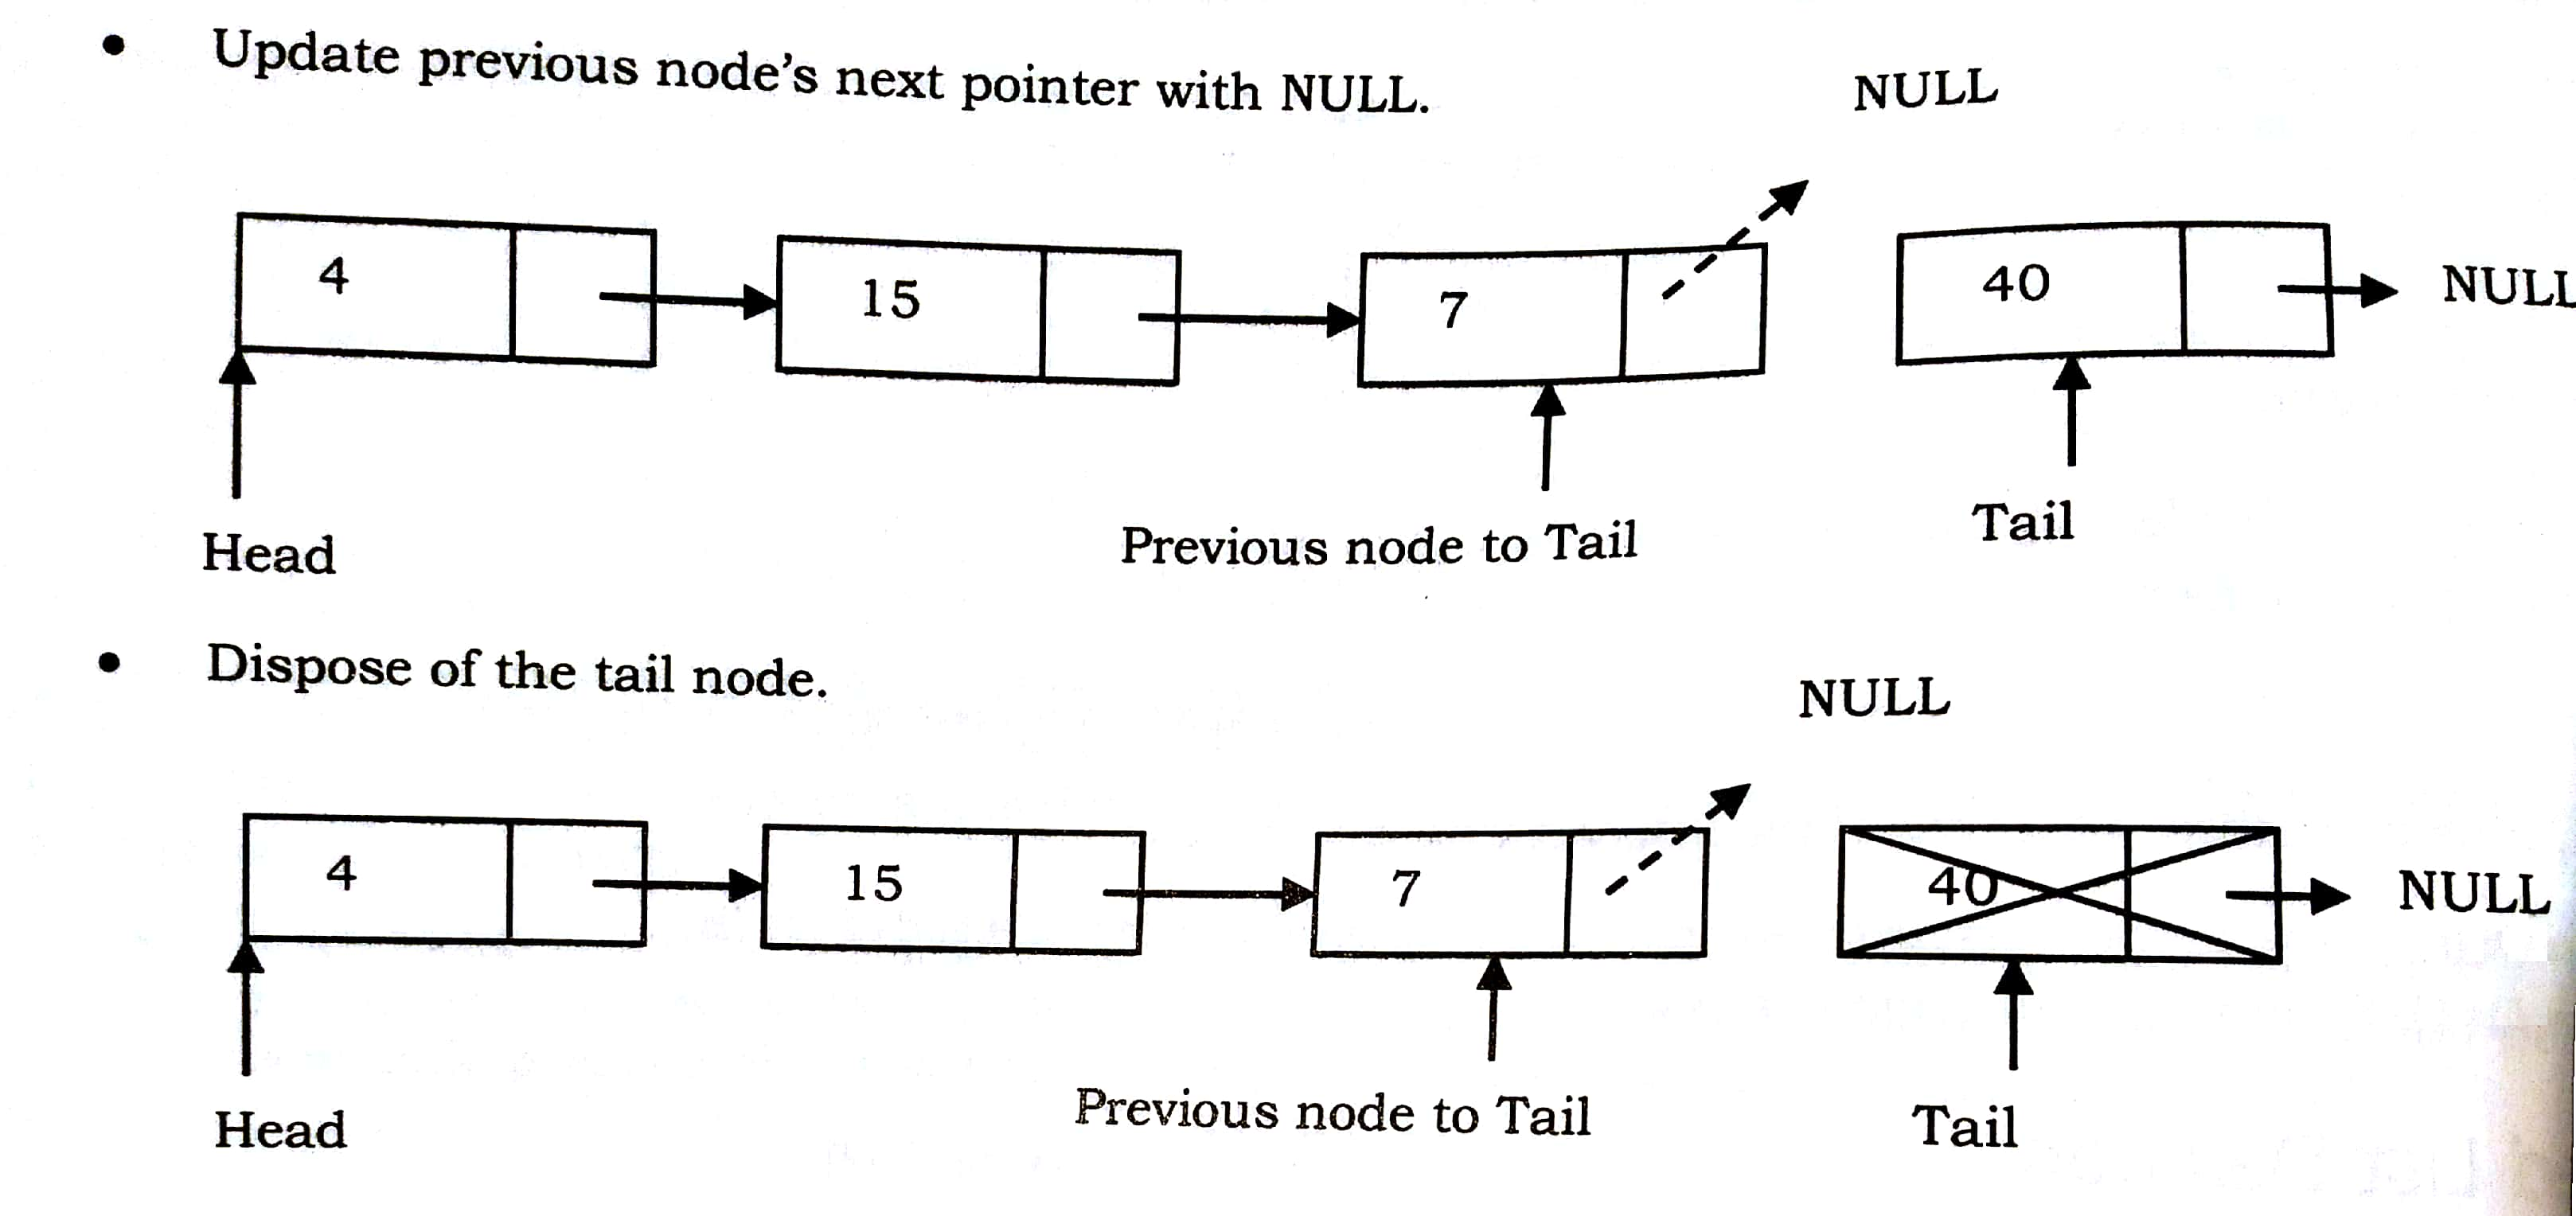
\includegraphics[height=0.50\paperheight, width=0.7\paperwidth]{figs/fig_listas/exclui_ultimo_no}						
			\caption{Exclui o último nó da lista}	
%%				\label{fig:lista-linear-repre}
		\end{figure} 

\end{frame} 


%----------------------------------------------------------------------------------------------------------


%----------------------------------------------------------------------------------------------------------

\begin{frame}%%%[allowframebreaks=0.98]

\frametitle{Listas Duplamente Encadeadas}

\begin{figure}[!hb]
	\centering
%%		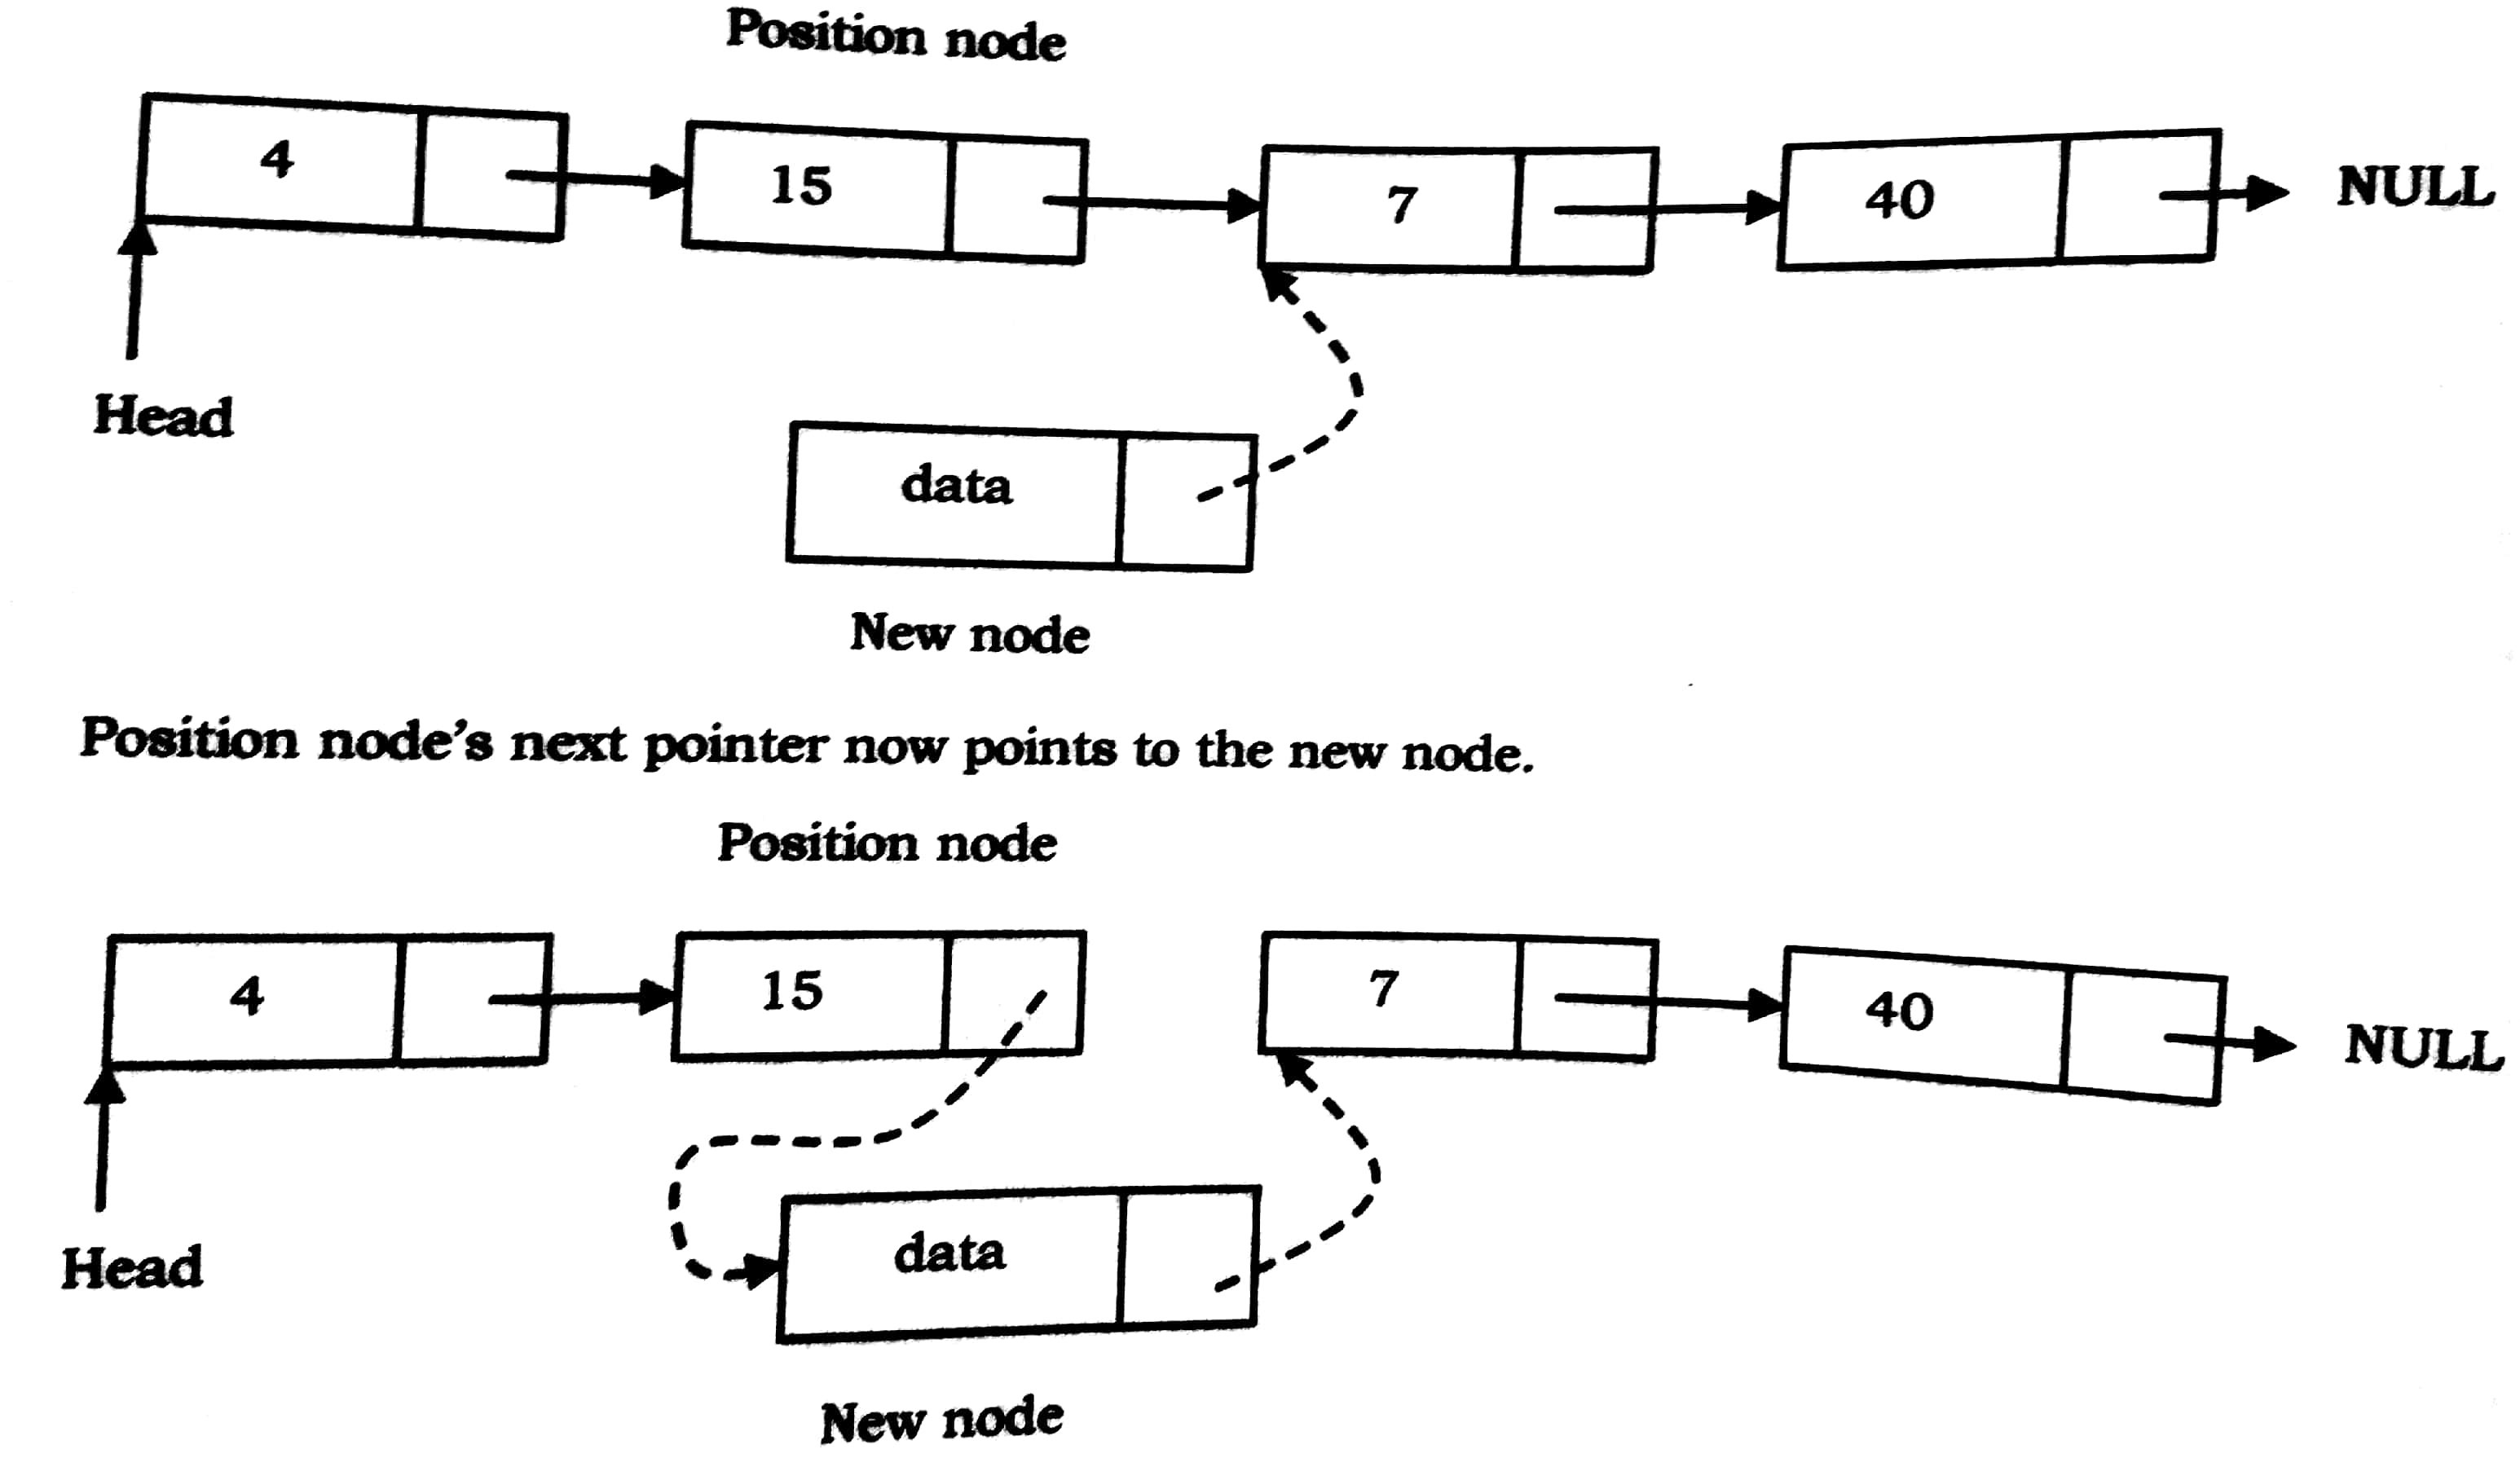
\includegraphics[scale=0.1]{figs/fig_listas/insere_posicao}
%%	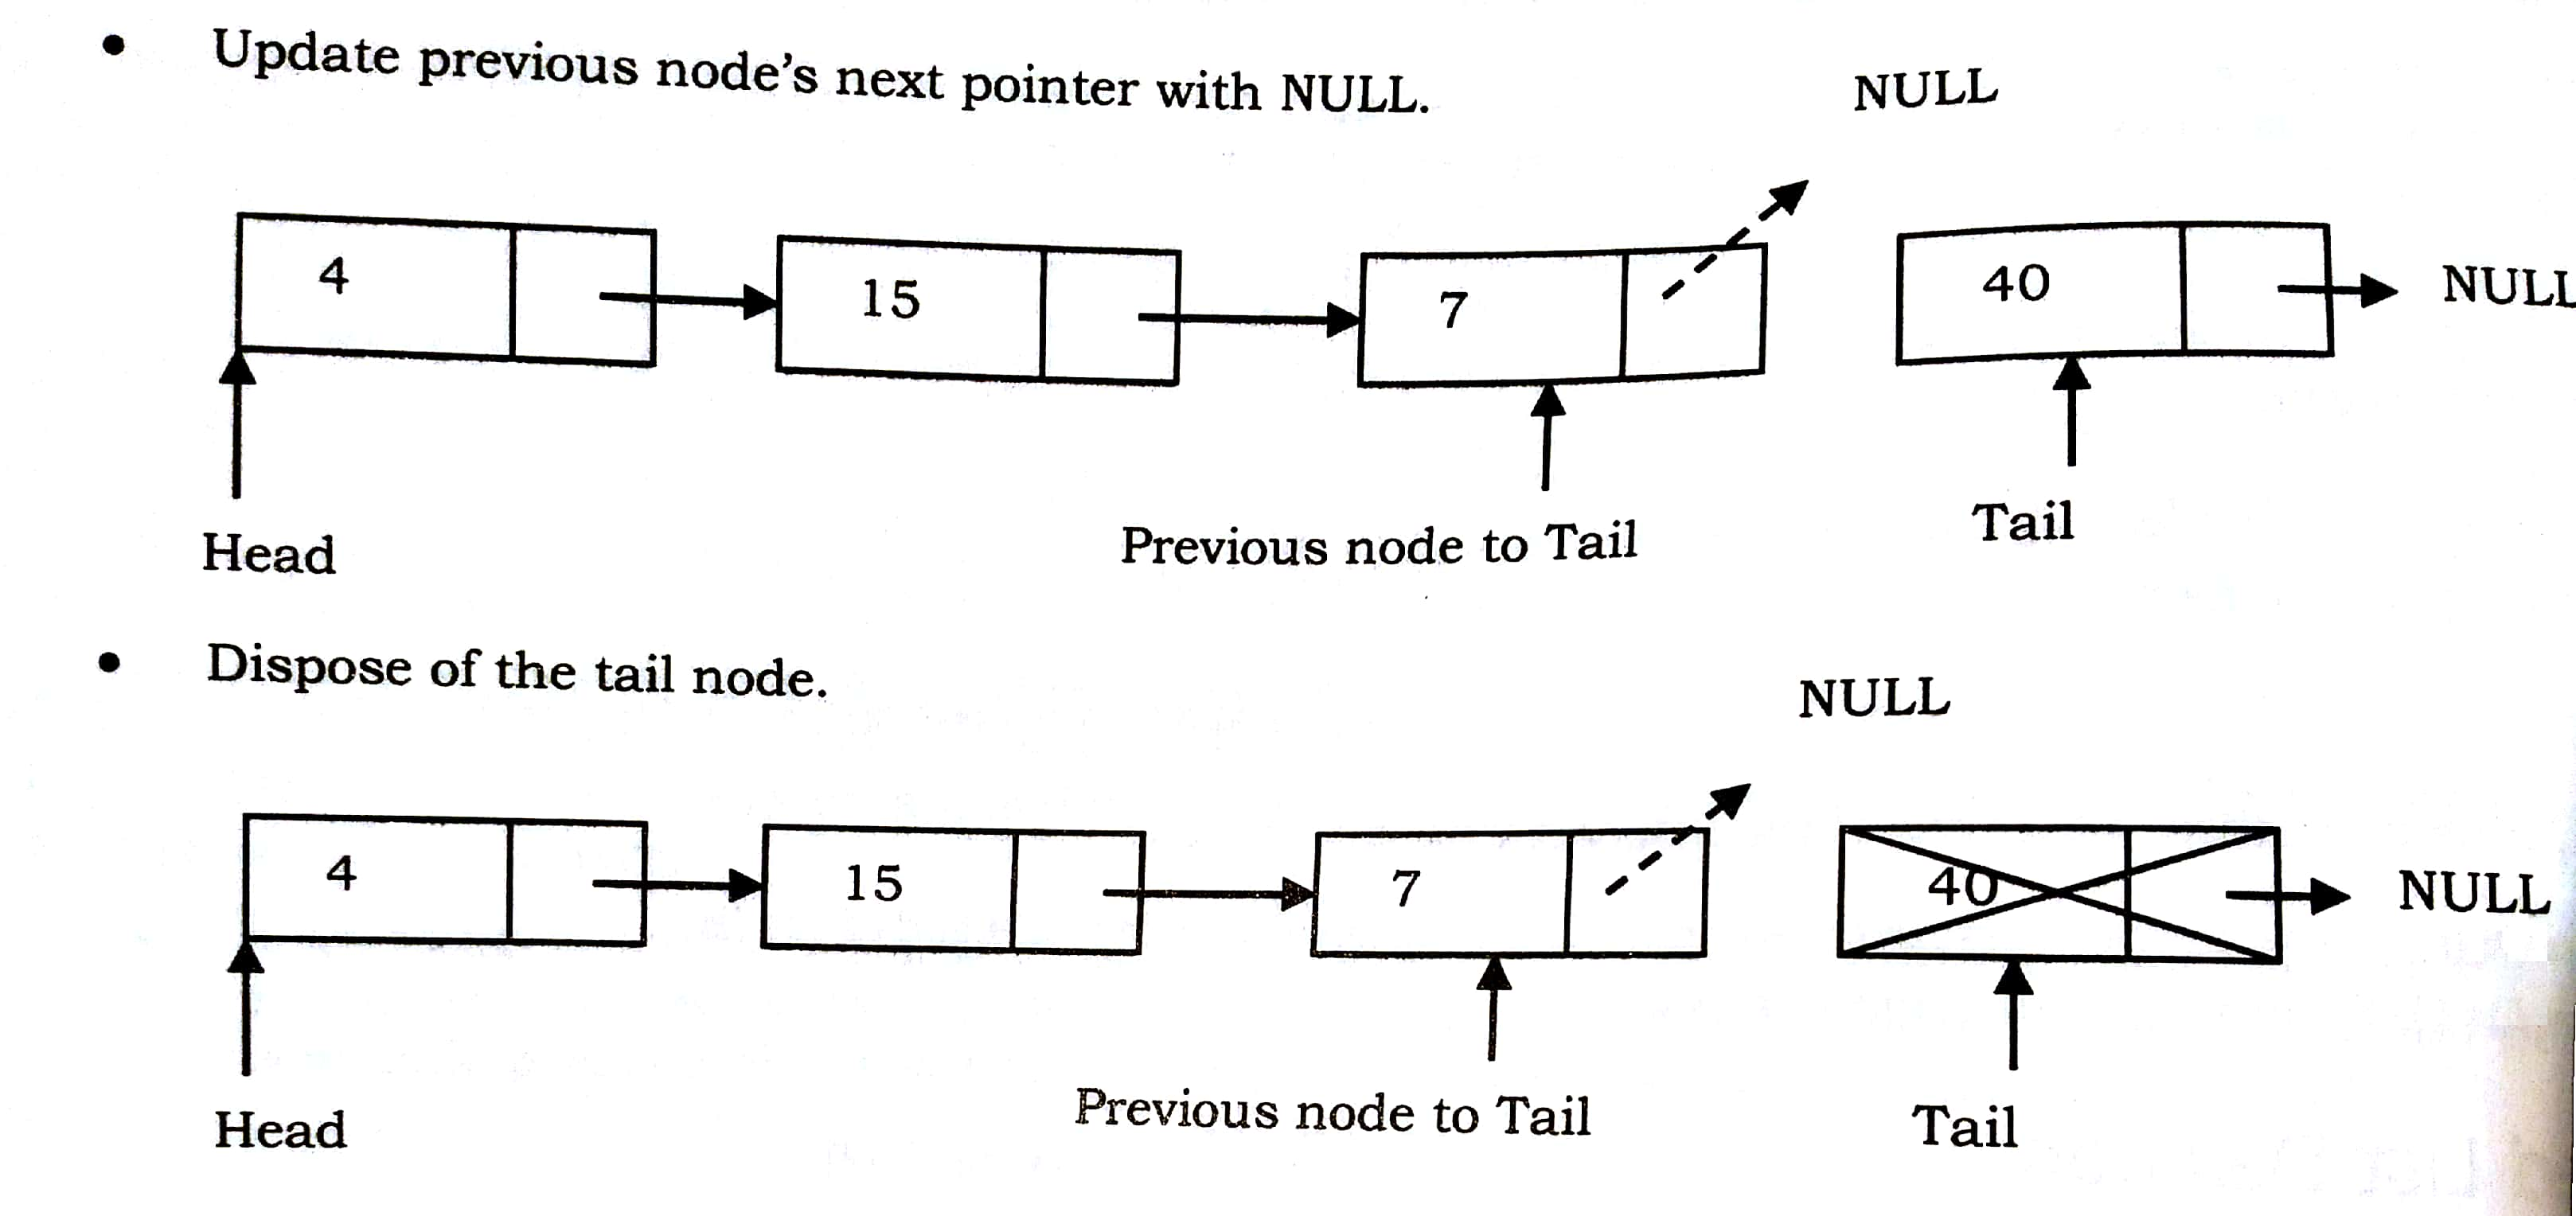
\includegraphics[height=0.50\paperheight, width=0.7\paperwidth]{figs/fig_listas/exclui_ultimo_no}						
			\caption{Listas Duplamente Encadeadas}	
%%				\label{fig:lista-linear-repre}
		\end{figure} 

\end{frame} 

%----------------------------------------------------------------------------------------------------------

\begin{frame}%%%[allowframebreaks=0.98]

\frametitle{Listas Circulares}

\begin{figure}[!hb]
	\centering
%%		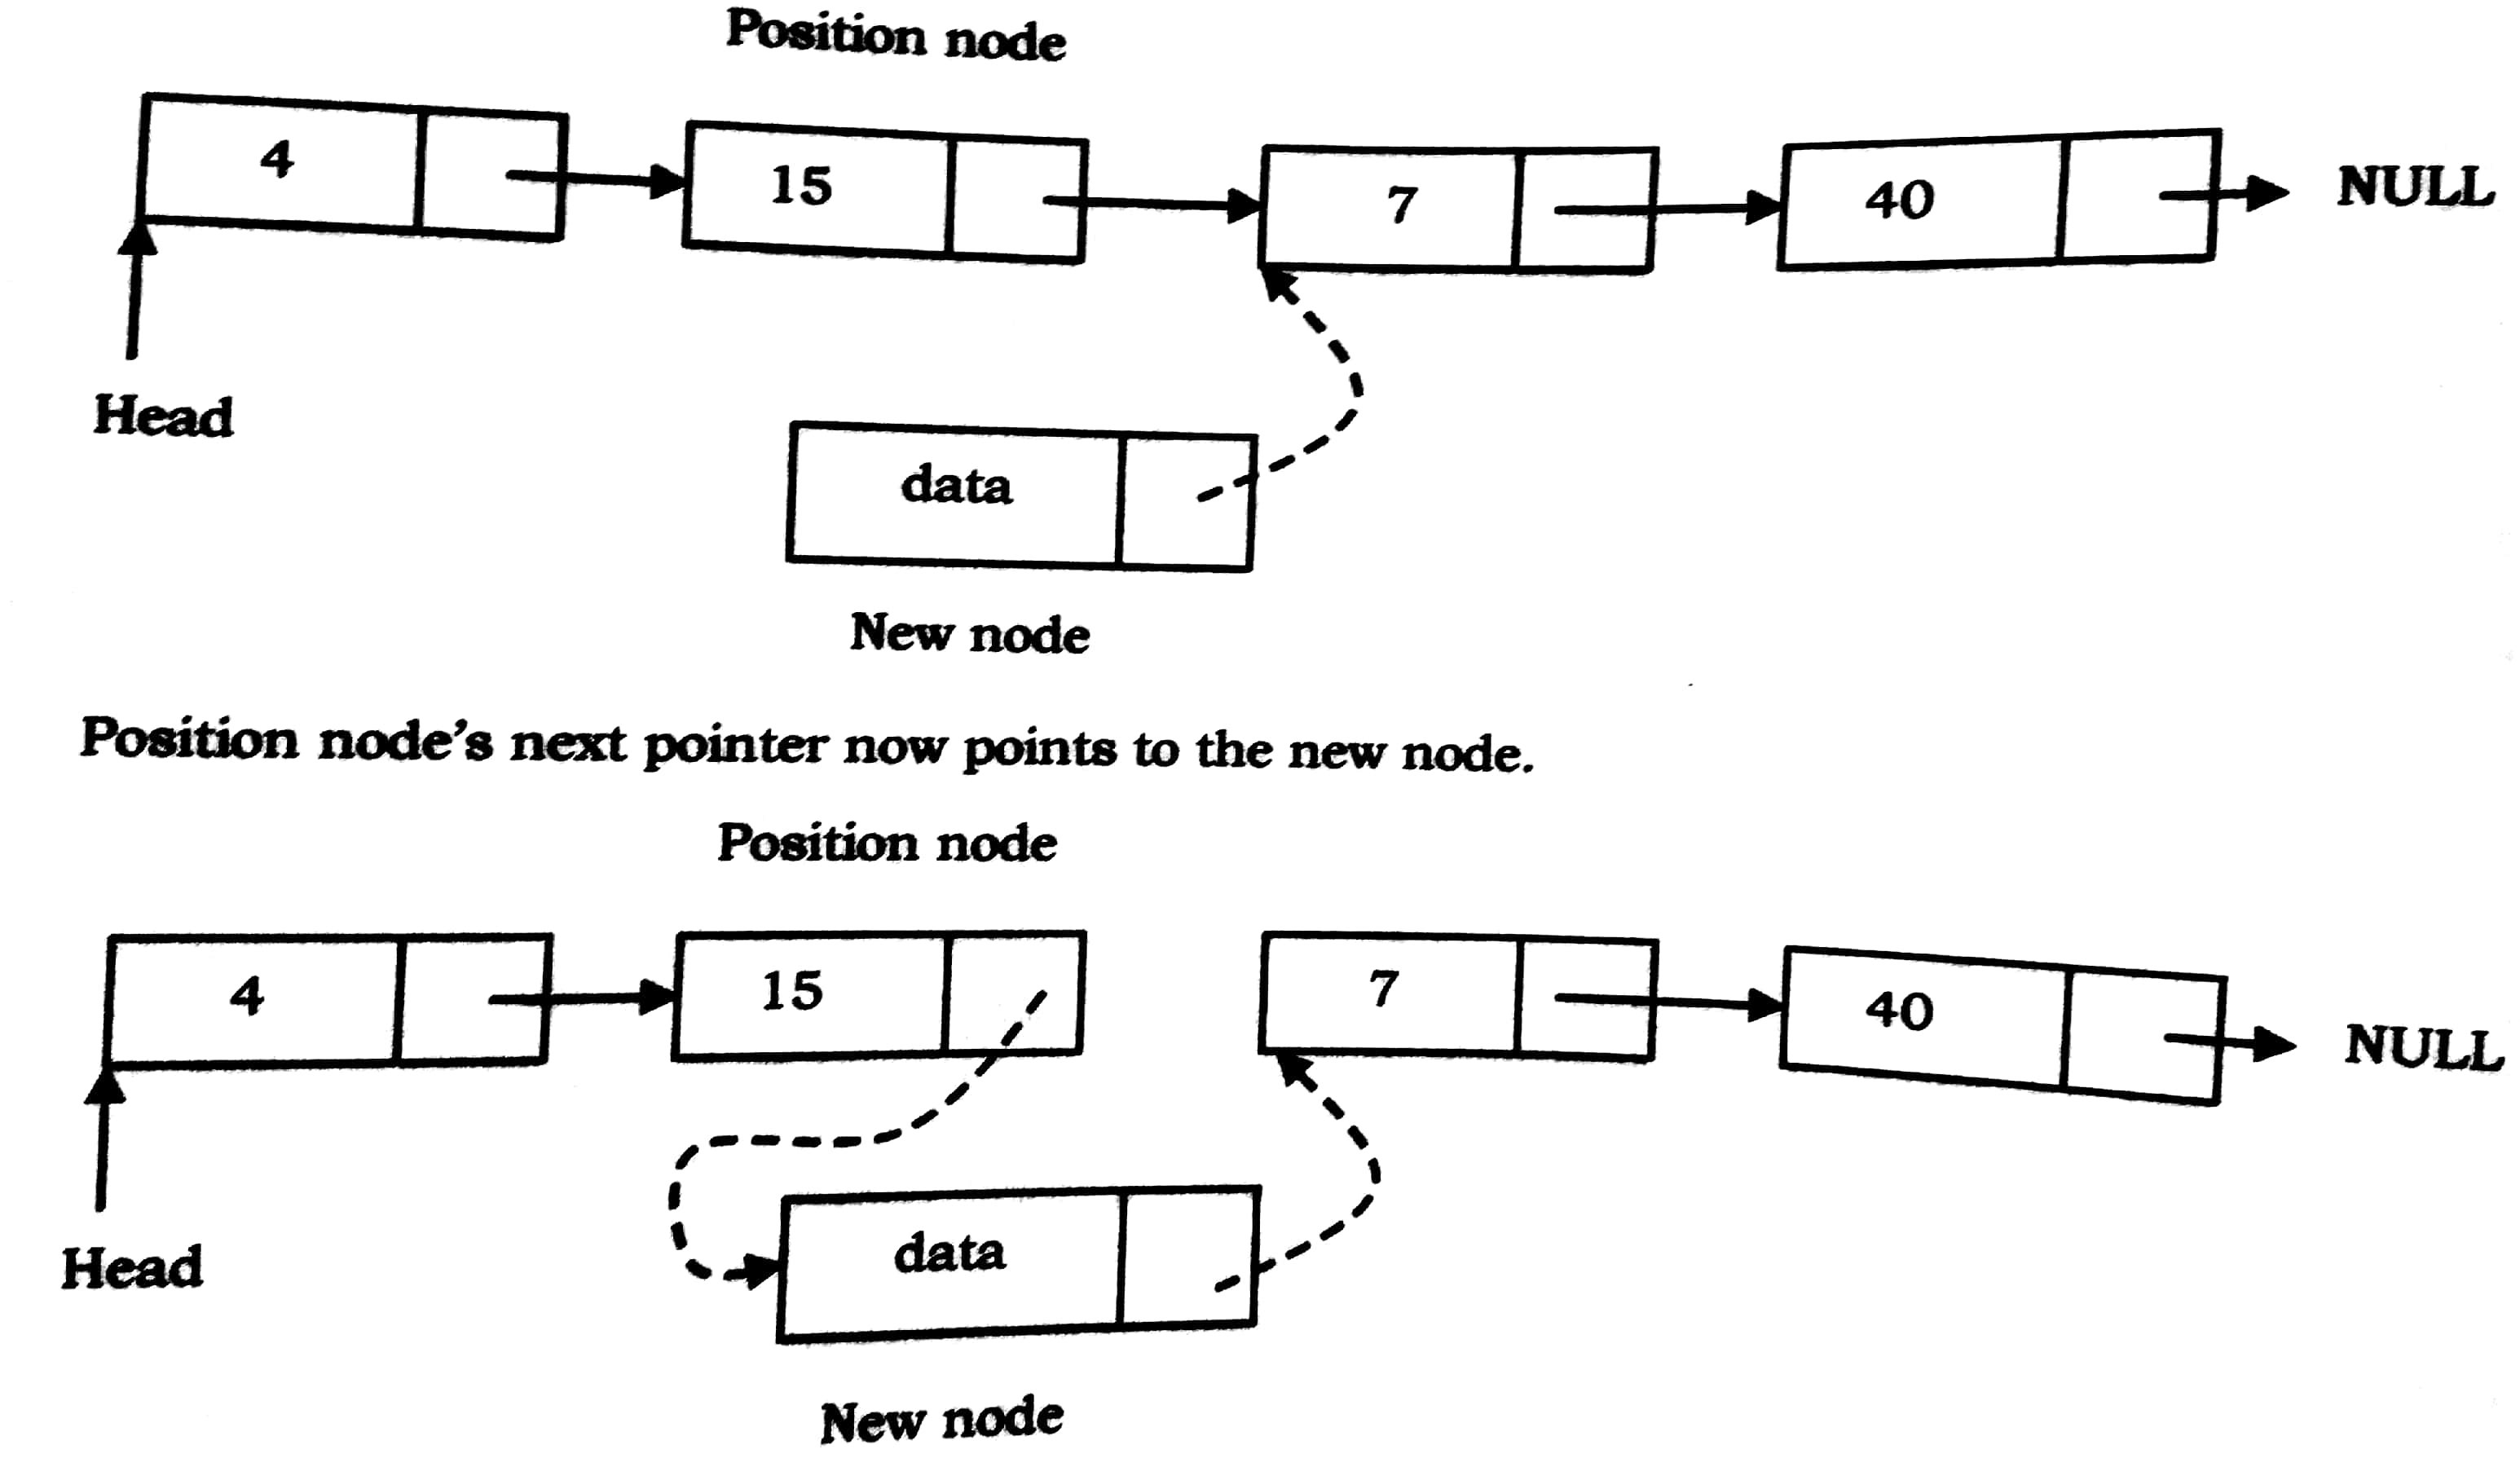
\includegraphics[scale=0.1]{figs/fig_listas/insere_posicao}
%%	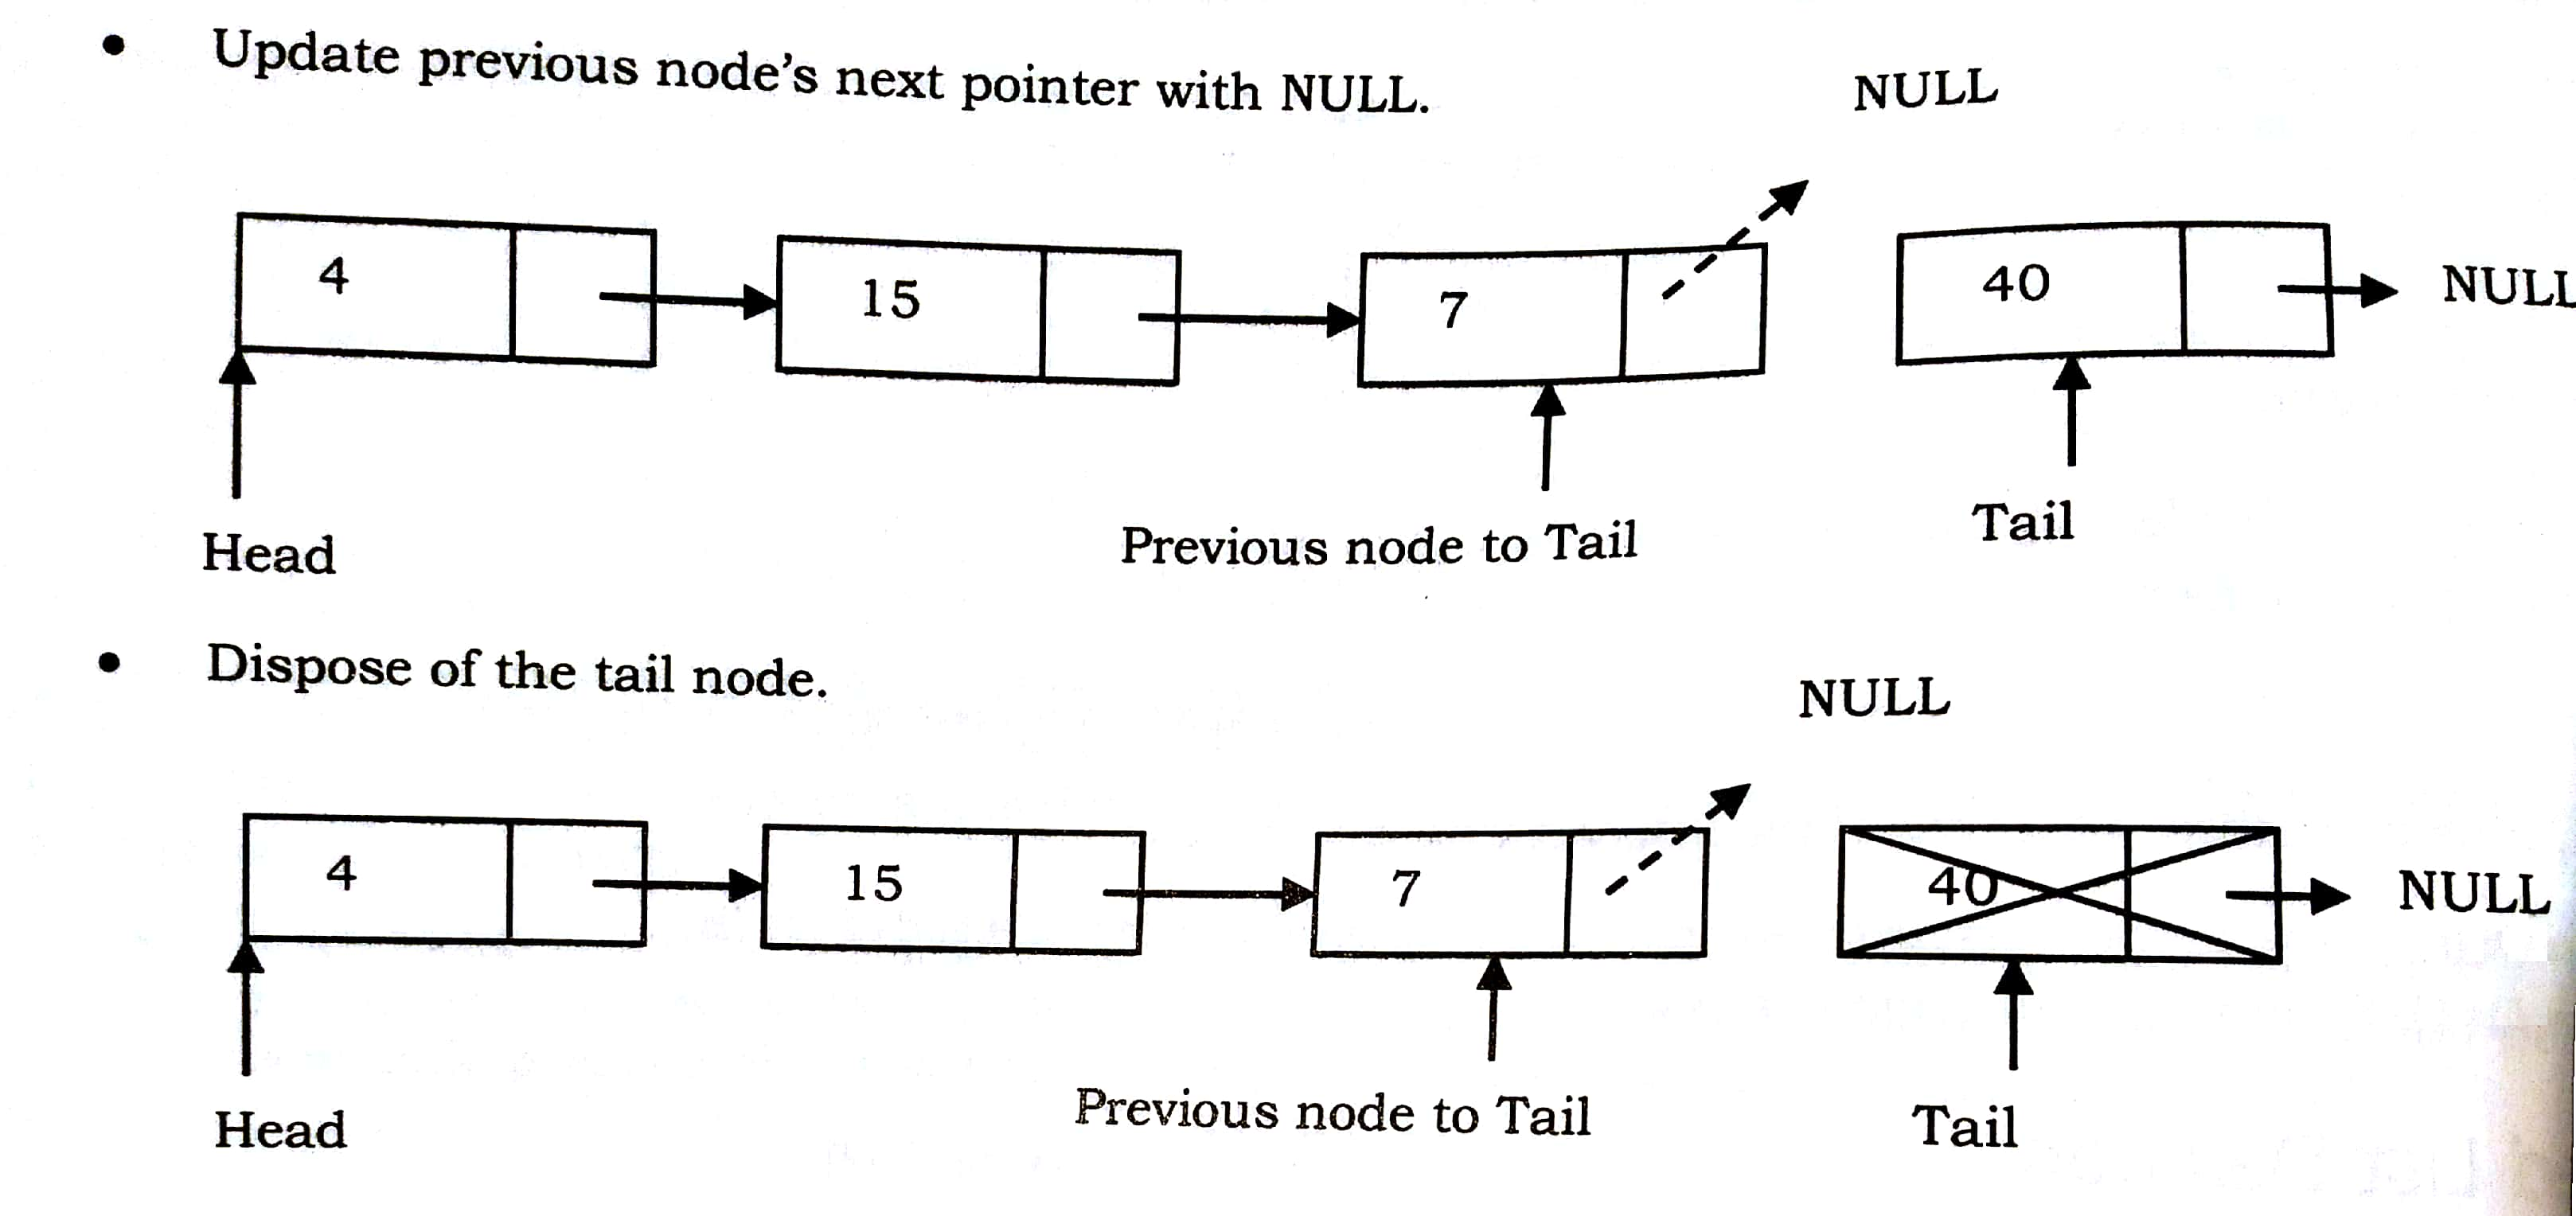
\includegraphics[height=0.50\paperheight, width=0.7\paperwidth]{figs/fig_listas/exclui_ultimo_no}						
			\caption{Listas Circulares}	
%%				\label{fig:lista-linear-repre}
		\end{figure} 

\end{frame} 

%ss------------------------------------------------------

\begin{frame}%%%[allowframebreaks=0.98]

\frametitle{Exercícios}

\begin{block}{Aqui esta \textit{lista} é grande ... }

\begin{itemize}
  \item Inverter a lista
  \item \textit{Merge} de duas listas
  \item 
  \item 
  \item 
  \item 
  
  
  
\end{itemize}


\end{block}


\end{frame} 

%%%%%%%%%%%------------------------------------------------------





\begin{frame}{Referências}
	\begin{enumerate}
	\item Karumanchi, Narashimha (2017). 
	\textit{Data Structures and Algorithms Made Easy -- Data Structures and Algorithms
		and Puzzles}.  CareerMonk.com

\item Tenenbaum, A. M., Langsam, Y., and Augestein, M. J. (1995). Estruturas de Dados Usando C. MAKRON Books, pp. 207-250.
\item Wirth, N. (1989). Algoritmos e Estrutura de dados. LTC, pp. 151-165.
	\end{enumerate}
\end{frame}
%----------------------------------------------------------------------------------------------------------

%%!TEX root = curso_EDA_SLIDES.tex

\section{Recursão}

\begin{frame}
\begin{center}
{\Large Capítulo xxxxx -- Recursão}

Pontos fundamentais a serem cobertos:

\begin{enumerate}
  \item 
  \item 
  \item 
\end{enumerate}

\end{center}

\end{frame}
%--------------------

\begin{frame}[fragile]{Recursão}
\begin{itemize}
	\item Um objeto é dito recursivo se ele consistir parcialmente ou for definido em termos de si próprio. Recursões não são encontradas apenas em matemática mas também no dia a dia. 
	\item Recursão é uma técnica particularmente poderosa em definições matemáticas. Alguns exemplos: números naturais, estrutura de árvore e certas funções:
	
\begin{enumerate}
	\item Números naturais:	
		\begin{enumerate}
			\item 0 é um número natural.
			\item O sucessor de um número natural é um número natural.
		\end{enumerate}
	\item Estruturas de árvores	
		\begin{enumerate}
			\item 0 é uma árvore (chamada árvore vazia).
			\item Se $t_1$ e $t_2$ são árvores, então a estrutura que consiste de um nó com dois ramos $t_1 \ e \ t_2$ também é uma arvore.			
		\end{enumerate}
	\item A função fatorial $n!$
	
\begin{enumerate}
	\item 0! = 1
	\item $n > 0, n! = n * (n - 1)$
\end{enumerate}
\end{enumerate}
\end{itemize}
\end{frame}  

\begin{frame}[fragile]{Recursão}
\begin{itemize}
	\item Se uma função $f$ possuir uma referência explícita a si próprio, então a função é dita \textit{diretamente recursiva}. Se $f$ contiver uma referência a outra função $g$, que por sua vez contém uma referência direta ou indireta a $f$, então $f$ é dita \textit{indiretamente recursiva}.
	\item Em termos matemáticos, a recursão é uma técnica que através de substituições sucessivas reduz o problema a ser resolvido a um caso de solução mais simples (Dividir para conquistar).
\end{itemize}
\end{frame}


\begin{frame}[fragile]{Recursão}
\framesubtitle{Exemplo}
\footnotesize
\begin{lstlisting}[language=C]
/**
 * Calcula a soma dos numeros inteiros 
 * existentes entre in e n inclusive.
 */
int somatorio(int in, int n){   
 int s = in;
 if (s < n)
 {      
   return s + somatorio(s + 1, n);
 }
 return s;
}

public static void main(String args)
{    
   print(somatorio(1, 100));
}
\end{lstlisting}
\end{frame}


\begin{frame}[fragile]{Recursão}
\begin{enumerate}
	\item Há dois requisitos-chave para garantir que a recursão tenha sucesso:	
			\begin{enumerate}
				\item Toda chamada recursiva tem de simplificar os cálculos de alguma maneira.
				\item Tem de haver casos especiais para tratar os cálculos mais simples diretamente.
			\end{enumerate}
	\item Muitas recursões podem ser calculadas com laços. Entretanto, as soluções iterativas para problemas recursivos podem ser mais complexas.
	\item Por exemplo, a permutação de uma palavra.
\end{enumerate}
\end{frame}

\begin{frame}[fragile]{Recursão}
\begin{itemize}
	\item A permutação é um exemplo de recursão que seria difícil de programar utilizando laços simples.
	\item Uma permutação de uma palavra é simplesmente um rearranjo das letras. Por exemplo, a palavra ``eat'' tem seis permutações ($n!$, onde $n$ é o número de letras que formam a palavra).
	\item Como gerar essas permutações?
	\item Simples, primeiro, gere todas as permutações que iniciam com a letra ``e'', depois as que iniciam com a letra ``a'' e finalmente as que iniciam com a letra ``t''.
	\item Mas, como gerar as permutações que iniciam com a letra ``e''?
	\item Gere as permutações da sub-palavra ``at''. Porém, esse é o mesmo problema, mas com uma entrada mais simples, ou seja, uma palavra menor.
	\item Logo, podemos usar a recursão nesse caso.
\end{itemize}
\end{frame}


\begin{frame}[fragile]{Recursão}
\begin{block}{Como pensar recursivo}  
		\begin{enumerate}
			\item Combine várias maneiras de simplificar as entradas.
			\item Combine as soluções de entradas mais simples para uma solução do problema original.
			\item Encontre soluções para as entradas mais simples.
			\item Implemente a solução combinando os casos simples e o passo de redução.
		\end{enumerate}
\end{block}
\end{frame}

\begin{frame}[fragile]{Eficiência da Recursão}
\begin{enumerate}
	\item A recursão pode ser uma ferramenta poderosa para implementar algoritmos complexos.
	\item No entanto, a recursão pode levar a algoritmos que tem um desempenho fraco.
	\item Vejamos quando a recursão é benéfica e quando é ineficiente.	
\end{enumerate}
\end{frame}

\begin{frame}[fragile]{Eficiência da Recursão}
\begin{enumerate}
	\item Considere a sequência de Fibonacci, uma sequência de números inteiros definidos pela equação:
	$$f_1 = 1$$
	$$f_2 = 1$$
	$$f_n = f_{n - 1} + f_{n - 2}$$
	\item Exemplo: $1,1,2,3,5,8,13,21,34,55, \ \cdots$.
	\item Vejamos uma implementação recursiva que calcule qualquer valor de $n$.	
\end{enumerate}
\end{frame}

\begin{frame}[fragile]{Eficiência da Recursão}
% \tiny{
\begin{lstlisting}[language=C]

  int fibonacci(int n) {				
    if (n <= 2)
      return 1;
    else
      return fibonacci(n - 1) + fibonacci(n - 2);		
  }

  void main(void) {
    int i;
    for (i = 1; i <= n; i++) {
      int f = fibonacci(i);
      printf("%d",  f);
    }
  }
}
\end{lstlisting}
% }
\end{frame}

\begin{frame}[fragile]{Eficiência da Recursão}

\begin{enumerate}
	\item Ao executarmos o programa de teste podemos notar que as primeiras chamadas à função \textbf{fibonacci} são bem rápidas. No entanto, para valores maiores, o programa pausa um tempo considerável entre as saídas.
	\item Inicialmente isso não faz sentido, uma vez que podemos calcular de forma rápida com auxílio de uma calculadora esses números, de modo que para o computador não deveria demorar tanto em hipótese alguma.
	\item Para descobrir o problema, vamos inserir mensagens de monitoração das funções e verificar a execução para $n = 6$.
\end{enumerate}
\end{frame}

\begin{frame}[fragile]{Eficiência da Recursão}
\tiny{
Início fibonacci n = 6\\
Início fibonacci n = 5\\
Início fibonacci n = 4\\
Início fibonacci n = 3\\
Início fibonacci n = 2\\
Término fibonacci n = 2, retorno = 1\\
Início fibonacci n = 1\\
Término fibonacci n = 1, retorno = 1\\
Término fibonacci n = 3, retorno = 2\\
Início fibonacci n = 2\\
Término fibonacci n = 2,\ retorno = 1\\
Término fibonacci n = 4, retorno = 3\\
Início fibonacci n = 3\\
Início fibonacci n = 2\\
Término fibonacci n = 2, retorno = 1\\
Início fibonacci n = 1\\
Término fibonacci n = 1, retorno = 1\\
Término fibonacci n = 3, retorno = 2\\
Término fibonacci n = 5, retorno = 5\\
Início fibonacci n = 4\\
Início fibonacci n = 3\\
Início fibonacci n = 2\\
Término fibonacci n = 2, retorno = 1\\
Início fibonacci n = 1\\
Término fibonacci n = 1, retorno = 1\\
Término fibonacci n = 3, retorno = 2\\
Início fibonacci n = 2\\
Término fibonacci n = 2, retorno = 1\\
Término fibonacci n = 4, retorno = 3\\
Término fibonacci n = 6, retorno = 8\\
Fibonacci(6) = 8\\
}
\end{frame}


\begin{frame}[fragile,plain]{Eficiência da Recursão}
\Tree [.f(6) [.f(5) [.f(4) [.f(3) f(2) f(1) ] f(2) ] [.f(3) f(2) f(1) ] ] [.f(4) [.f(3) f(2) f(1) ] f(2) ] ] 

\begin{center} Padrão de chamada de função/método recursivo \textit{fibonacci}. \end{center}
\end{frame}

\begin{frame}[fragile,plain]{Eficiência da Recursão}
\begin{enumerate}
	\item Analisando o rastro de execução do programa fica claro porque o método leva tanto tempo. 
	\item Ele calcula os mesmos valores repetidas vezes.
	\item Pelo exemplo, o calculo de \textbf{fibonacci(6)} chama \textbf{fibonacci(4)} duas vezes, \textbf{fibonacci(3)} três vezes, \textbf{fibonacci(2)} cinco vezes, e \textbf{fibonacci(1)} três vezes. 
	\item Diferente do cálculo que faríamos manualmente.
\end{enumerate}

\Tree [.f(6) [.f(5) [.\textcolor{red}{f(4)} [.\textcolor{blue}{f(3)} \textcolor{green}{f(2)} f(1) ] \textcolor{green}{f(2)} ] [.\textcolor{blue}{f(3)} \textcolor{green}{f(2)} f(1) ] ] [.\textcolor{red}{f(4)} [.\textcolor{blue}{f(3)} \textcolor{green}{f(2)} f(1) ] \textcolor{green}{f(2)} ] ] 
\end{frame}

\begin{frame}[fragile,plain]{Em resumo...}
\begin{block}{Eficiência da Recursão}
As vezes acontece de uma solução recursiva ser executada muito mais lentamente do que sua equivalente iterativa. Entretanto, na maioria dos casos, a solução recursiva é apenas levemente mais lenta.
\end{block}
\begin{block}{}
Em muitos casos, uma solução recursiva é mais fácil de entender e implementar corretamente do que uma solução iterativa.
\end{block}
\end{frame}
 % cap 0
%\section{Introdução}
\section{Árvores}

\begin{frame}

\begin{center}
{\Large Capítulo 06 -- Árvores}
\end{center}

Pontos fundamentais a serem cobertos:
\begin{columns}
\begin{column}{.3\textwidth}
\centering

  \begin{enumerate}
  \item Contexto e motivação

  \item Definição

  \item Implementações

  \item Exercícios 

\end{enumerate}  

\end{column}
\begin{column}{.7\textwidth}
\centering
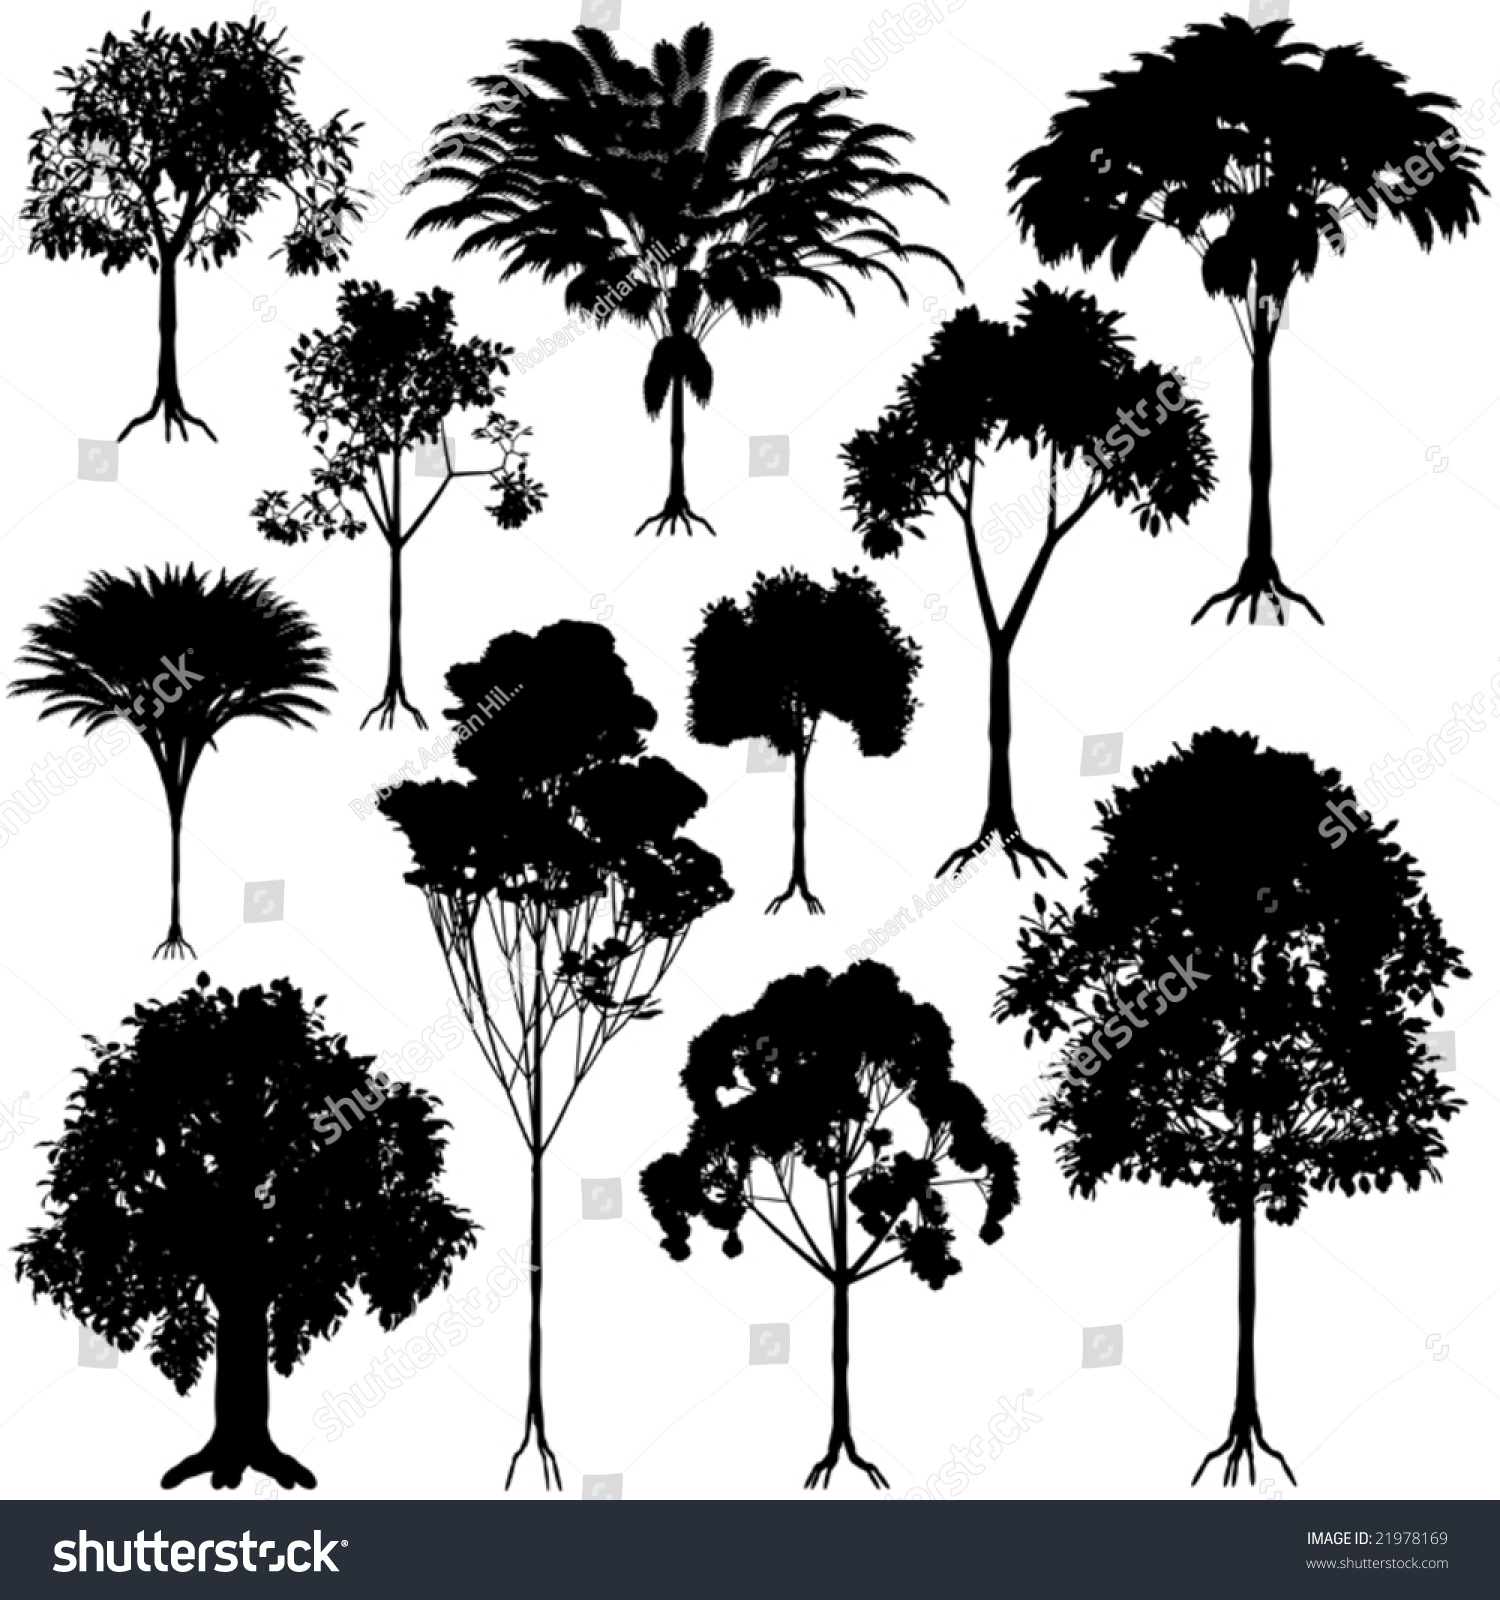
\includegraphics[height=5.3cm, width=7cm]{figs/fig_arvores/arv_CAPA.jpg}
\hspace{+0.25cm}
%\scriptsize\textcolor{red}{[Tizio, Caio et al., Nature (2006)]}
\end{column}
\end{columns}


\end{frame}
%-----------------------------------------------------------------------------
\subsection{Apresentação}

\begin{frame}%[allowframebreaks=0.9, c]

    \frametitle{Definição}
    
    \begin{itemize}
    \item Uma árvore é uma estrutura hierárquica composta por nós e ligações entre eles
    \item Pode ser vista como um grafo acíclico
    \item Cada nó possui somente um pai e zero ou mais filhos
    \item Muitas definições ...
    \end{itemize}
\end{frame}

%---------------------------------------------------------
\begin{frame}%[allowframebreaks=0.9, c]
    \frametitle{Estrutura}
    
    \begin{figure}[tbp]
    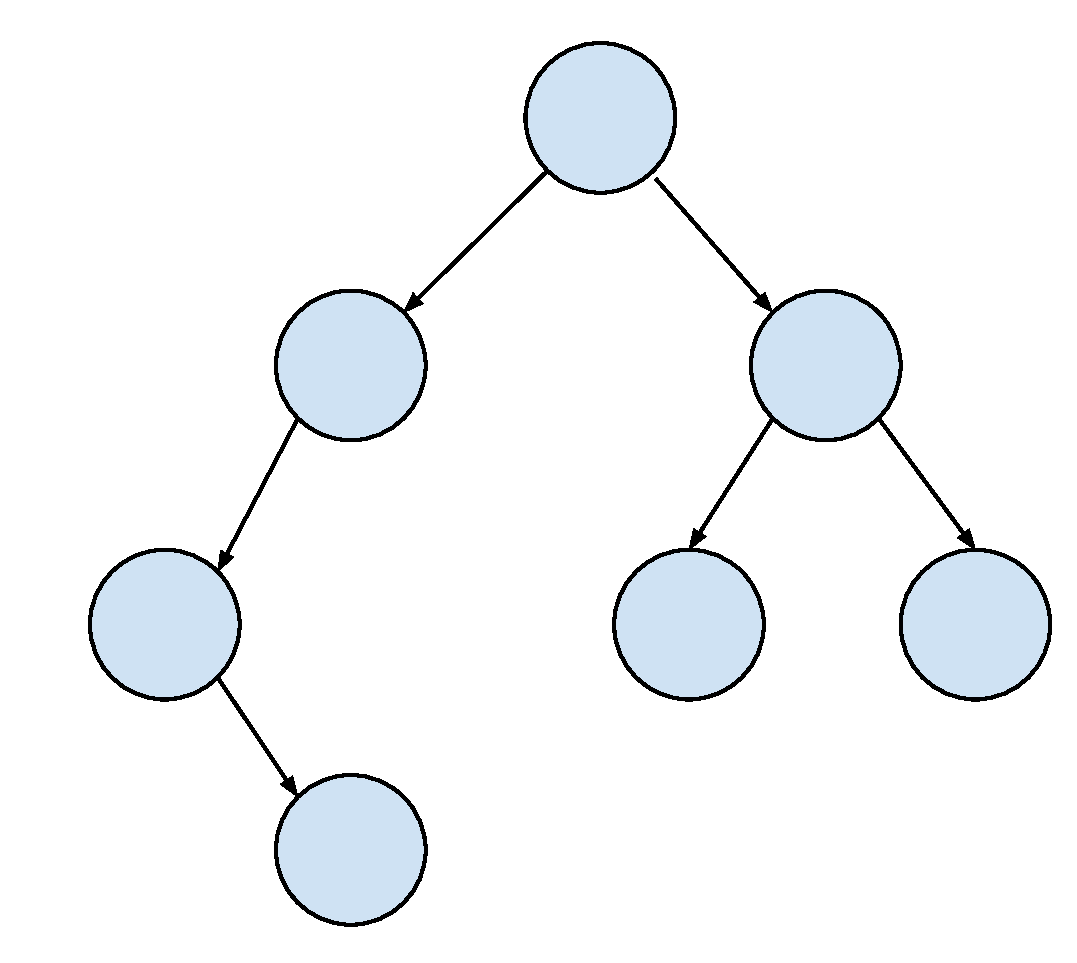
\includegraphics[keepaspectratio=true,width=2.5in]{figs/fig_arvores/arvore.pdf}
    \centering
    \caption{Exemplo de uma árvore}
    \end{figure}
\end{frame}
%---------------------------------------------------------


%---------------------------------------------------------
\begin{frame}
    \frametitle{\textit{Roadmap} para estudo}
    
\begin{block}{mantendo um \textit{foco}:}

\begin{enumerate}
  \item Conceitos de árvores genéricas etc ... 
    \item Árvores Binárias
  \item Árvore Binária de Busca
   \item Árvore AVL (iniciais dos nomes:  \textit{Georgii Adelson-Velsky et Evguenii Landis (en), 
   qui l'ont publié en 1962 sous le titre An Algorithm for the Organization of Information})
   \item Projeto 10\% : 
   \begin{itemize}
     \item  Implemente uma AVL;
    \item   Leia um conjunto de dados numéricos contidos no arquivo fornecido (um valor por linha: string, int, float, char), inserindo-os sequencialmente na AVL implementada;
    \item   Imprima o percurso (valores dos nós) em pré-ordem, em-ordem e pós-ordem, além da altura da árvore
    \item Com a altura dará para ver se a AVL está OK!
   \end{itemize}
  
  \item Vídeos bem legais no Youtube da UNIVEST
  
\end{enumerate}


\end{block}



    \end{frame}

%---------------------------------------------------------
\begin{frame}
    \frametitle{Características -- Requisitos}
    
\begin{itemize}
  
  \item  Como é um nó?
  \item  Qual o grau de um nó?
  \item  Como devem estar estruturados os valores dos nós?
  \item  O que é uma chave do nó?
  \item  O que é a altura?
  \item  Nível?
  \item  Caminhos

\end{itemize}


\end{frame}

%-------------------------------------------------------------------------------------------------------------
\begin{frame}

    \frametitle{Glossário -- 01}
    
     \begin{figure}[!ht]
     \centering
    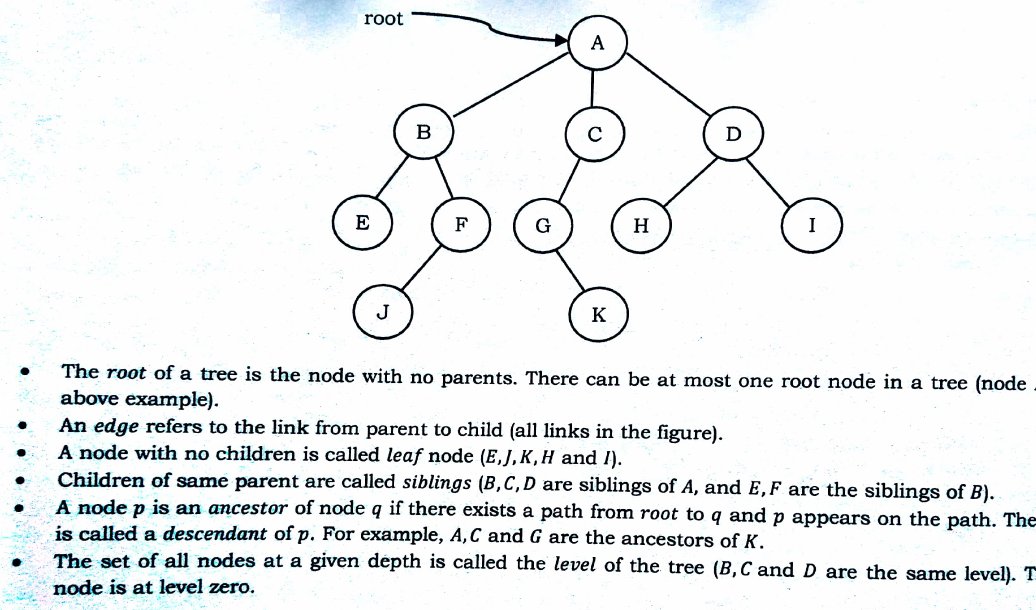
\includegraphics[width=12cm, height=7cm]{figs/fig_arvores/glossario_arv_01.png}
    %\caption{\textcolor{red}{Usando os problemas de árvores genéricas para apresentar Árvores Binárias (AB) }}
    \end{figure}

\end{frame}

%-------------------------------------------------------------------------------------------------------------
\begin{frame}

    \frametitle{Glossário -- 02}
    
     \begin{figure}[!ht]
     \centering
    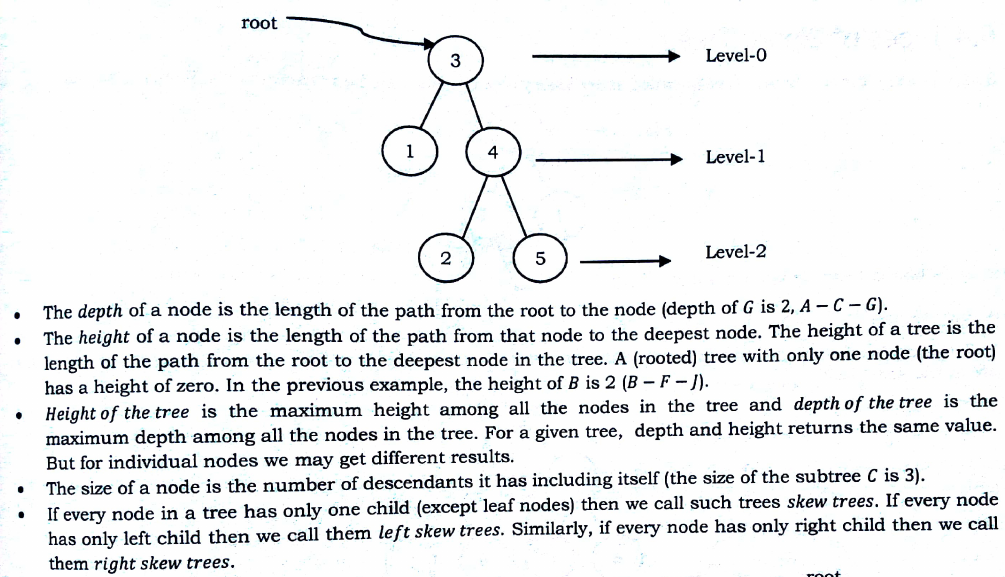
\includegraphics[width=12cm, height=7cm]{figs/fig_arvores/glossario_arv_02.png}
    %\caption{\textcolor{red}{Usando os problemas de árvores genéricas para apresentar Árvores Binárias (AB) }}
    \end{figure}

\end{frame}
%-------------------------------------------------------------------------------------------------------------
\begin{frame}

    \frametitle{Glossário -- 03}
    
     \begin{figure}[!ht]
     \centering
    \includegraphics[width=8cm, height=5cm]{figs/fig_arvores/glossario_arv_03.png}
    %\caption{\textcolor{red}{Usando os problemas de árvores genéricas para apresentar Árvores Binárias (AB) }}
    \end{figure}

\end{frame}

%-------------------------------------------------------------------------------------------------------------

\subsection{Árvores Genéricas}

\begin{frame}

    \frametitle{Árvores Genéricas}
    %%Representação  Computacional de 
     \begin{figure}[!ht]
     \centering
    \includegraphics[width=9cm, height=5cm]{figs/fig_arvores/arv_generica01.jpg}
    \caption{\textcolor{red}{Usando os problemas de árvores genéricas para apresentar Árvores Binárias (AB) }}
    \end{figure}

\end{frame}
%-------------------------------------------------------------------------------------------------------------

\begin{frame}

    \frametitle{Transformando uma Árvore Genérica em Binária}
    
     \begin{figure}[!ht]
     \centering
    \includegraphics[width=10cm, height=5cm]{figs/fig_arvores/arv_generica02.jpg}
    \caption{\textcolor{red}{Usando os problemas de árvores genéricas para apresentar Árvores Binárias(AB)}}
    \end{figure}

\end{frame}

%-------------------------------------------------------------------------------------------------------------

\begin{frame}

    \frametitle{Representação  Computacional de uma Árvore Genérica}
    
     \begin{figure}[!ht]
     \centering
    \includegraphics[width=10cm, height=5cm]{figs/fig_arvores/arv_generica03.jpg}
    \caption{\textcolor{red}{Felizmente há um algoritmo que transforme  Árvores Genéricas em Binárias (AB) }}
    \end{figure}

\end{frame}
%-------------------------------------------------------------------------------------------------------------

\begin{frame}

    \frametitle{Representação  Computacional de uma Árvore Genérica}
    
     \begin{figure}[!ht]
     \centering
    \includegraphics[width=10cm, height=6cm]{figs/fig_arvores/arv_generica04.png}
   \caption{\textcolor{red}{Veja a \textit{struct} ... lembra o quê?}}
    \end{figure}

\end{frame}

%---------------------------------------------------------

\subsection{Aplicações}

\begin{frame}

    \frametitle{Aplicações}

    \begin{itemize}
      \item  Área de compiladores: análise sintática 
      \item  Buscas com complexidade na ordem de: $O(\log n)$ 
     % \item  O uso de Árvores Genéricas foi apenas para motivar as ABBs
      \item  Na área de IA para construção de árvores de decisão: mineração de dados (\textit{big data})
      \item  Organização de taxonomias de conhecimento
      \item  Estruturas hierárquicas em geral      
      
    \end{itemize}    
    
\end{frame}


%---------------------------------------------------------

\begin{frame}

\frametitle{Aplicação  de Árvores}

  \begin{figure}[!ht]
     \centering
    \includegraphics[width=7cm, height=5.5cm]{figs/fig_arvores/aplicacao_decision_tree.png}
    \caption{Árvore de Decisão}
    \end{figure}

\end{frame}

%---------------------------------------------------------

\begin{frame}

    \frametitle{Aplicação  de Árvores}

  \begin{figure}[!ht]
     \centering
    \includegraphics[width=7cm, height=5.5cm]{figs/fig_arvores/aplicacao_expression_tree.png}
    \caption{Árvores de expressões -- binárias -- novamente}
    \end{figure}

\end{frame}

%---------------------------------------------------------

\subsection{Árvore Binária de Busca}

\frame{
    \frametitle{Árvores Binárias de Buscas - ABBs}
    
    
    \begin{itemize}
      \item Árvores Genéricas (AGs): foram utilizadas para motivação as ABBs
      \item Computacionalmente, as ABBs tem um interesse maior que as AGs
      \item Assim, se inicia com ABBs, e seus algoritmos serão adaptados as AGs
    \end{itemize}
    \pause
    
\begin{block}{Definição:}
        
    Árvore onde cada nó possui até 2 filhos. O filho da esquerda só pode conter
    chaves menores do que a do pai, enquanto que o filho da direita só comporta chaves
    maiores do que a do pai.
    \end{block}

}

%---------------------------------------------------------
\frame{
    \frametitle{Árvore Binária de Busca}
    
    \begin{figure}[tbp]
    \includegraphics[keepaspectratio=true,width=3in]{figs/fig_arvores/arvore_binaria_de_busca}
    \centering
    \caption{Exemplo de árvore binária de busca}
    \end{figure}
}

%---------------------------------------------------------
\begin{frame}
    \frametitle{Árvore Binária de Busca}
    
    \begin{figure}[tbp]
    \includegraphics[keepaspectratio=true,width=4in]{figs/fig_arvores/no}
    \centering
    \caption{Estrutura básica / nó}
    \end{figure}

\end{frame}

%---------------------------------------------------------
\frame{
    \frametitle{Operações Básicas}
    
    \begin{block}{Operações Básicas}
    \begin{itemize}
    \item Inserção
    \item Busca
    \item Remoção -- faltando
    \end{itemize}
    \end{block}
    
    \begin{block}{Usos Comuns}
    \begin{itemize}
    \item Dicionários / vetores associativos
    \item Filas de prioridades
    \end{itemize}
    \end{block}
}

%---------------------------------------------------------
\frame{
    \frametitle{Complexidade Computacional}
    
    Quando a árvore está balanceada todas as três operações podem ser implementadas com complexidade
    computacional igual a $O(\log n)$.
    \\ [2em]
    No pior caso (desbalanceamento) estas operações possuem complexidade $O(n)$~\cite{cormen}.
}

%---------------------------------------------------------
\begin{frame}[fragile]
\frametitle{Árvore Binária de Busca - Inserção}
\begin{verbatim}
INSERÇÃO(ARVORE, ITEM) {
    SE ARVORE->CHAVE == NULO
       ARVORE->ITEM = ITEM
       return      //e SE CHAVE jah existente?

    SE ITEM->CHAVE < ARVORE->CHAVE
        SE ARVORE->ESQ = NULO ENTÃO
            ARVORE->ESQ = ARVORE(ITEM)
        SENÃO
            INSERÇÃO(ARVORE->ESQ, ITEM)
    SENÃO
        SE ARVORE->DIR = NULO ENTÃO
            ARVORE->DIR = ARVORE(ITEM)
        SENÃO
            INSERÇÃO(ARVORE->DIR, ITEM)
}
\end{verbatim}
\end{frame}

%---------------------------------------------------------
\frame{
    \frametitle{Árvore Binária de Busca - Inserção}
    
    \begin{figure}[tbp]
    \includegraphics[keepaspectratio=true,width=3in]{figs/fig_arvores/insercao_1}
    \centering
    \caption{Exemplo de inserção da chave 40}
    \end{figure}
}

%---------------------------------------------------------
\frame{
    \frametitle{Árvore Binária de Busca - Inserção}
    
    \begin{figure}[tbp]
    \includegraphics[keepaspectratio=true,width=3in]{figs/fig_arvores/insercao_2}
    \centering
    \caption{Exemplo de inserção da chave 20}
    \end{figure}
}

%---------------------------------------------------------
\begin{frame}[fragile]
\frametitle{Árvore Binária de Busca - Busca}
\begin{verbatim}
BUSCA(ARVORE, CHAVE) {
    SE ARVORE = NULO
        return NULO
        
    SE ARVORE->CHAVE = CHAVE
        return ARVORE
    
    SE CHAVE < ARVORE->CHAVE
        return BUSCA(ARVORE->ESQ, CHAVE)
    SENÃO
        return BUSCA(ARVORE->DIR, CHAVE)
}
\end{verbatim}
\end{frame}

%---------------------------------------------------------
\frame{
    \frametitle{Árvore Binária de Busca -- Remoção}
    
    A remoção de um nó se enquadra em um dos seguintes casos:
    
    \begin{enumerate}
    \item Remoção de um nó folha (nenhum filho)
    \item Remoção de um nó com somente um filho
    \item Remoção de um nó com dois filhos
    \item  \textcolor{red}{Faltam as figuras ainda ....}
    \end{enumerate}

   %% O tratamento de cada caso foi apresentado em sala de aula.
}

%---------------------------------------------------------
\subsection{Balanceamento}

\frame{
    \frametitle{Balanceamento}
    
    Uma árvore binária de busca balanceada garante operações de busca, inserção e
    remoção com complexidade O($\log n$), onde $n$ é o número de nós, o que a torna atrativa
    para diversas aplicações.
    \\[1em]
    Determinadas sequências de inserções ou remoções podem fazer com que uma ABB fique
    desbalanceada, tornando suas operações O($n$).
}

\begin{frame}[fragile]
\frametitle{Cálculo da Altura}
\begin{verbatim}
ALTURA(ARVORE) {
    SE ARVORE = NULO
        return -1
        
    A1 = ALTURA(ARVORE->DIR)
    A2 = ALTURA(ARVORE->ESQ)
    
    return maior(A1, A2) + 1
}
\end{verbatim}
\end{frame}

%---------------------------------------------------------
\begin{frame}
\frametitle{Cálculo da Altura}

\begin{figure}[tbp]
\includegraphics[keepaspectratio=true,width=3in]{figs/fig_arvores/altura1}
\centering
\caption{Exercício: determine a altura de cada subárvore.}
\end{figure}

\end{frame}

%---------------------------------------------------------
\begin{frame}
\frametitle{Cálculo da Altura}

\begin{figure}[tbp]
\includegraphics[keepaspectratio=true,width=3in]{figs/fig_arvores/altura2}
\centering
\caption{Resposta do exercício.}
\end{figure}

\end{frame}

%---------------------------------------------------------
\begin{frame}[fragile]
\frametitle{Cálculo do Fator de Balanceamento}
\begin{verbatim}
FB(ARVORE) {
    A1 = ALTURA(ARVORE->ESQ)
    A2 = ALTURA(ARVORE->DIR)
    return A1 - A2 
}
\end{verbatim}
\end{frame}

%---------------------------------------------------------
\frame{
    \frametitle{Balanceamento}
    
    \begin{itemize}
    \item Uma ABB está balanceada quando cada nó possui um FB igual a -1, 0 ou 1
    \item Uma inserção ou remoção pode tornar uma árvore desbalanceada, necessitando de rotações
    para o seu balanceamento
    \end{itemize}
}

%---------------------------------------------------------
\begin{frame}
    \frametitle{Exemplo de ABB Balanceada}
    
    \begin{figure}[tbp]
    \includegraphics[keepaspectratio=true,width=3in]{figs/fig_arvores/Balanceamento_Arvore}
    \centering
    \end{figure}
\end{frame}

%---------------------------------------------------------
\begin{frame}
    \frametitle{Exemplo de ABB Desbalanceada}
    
    \begin{figure}[tbp]
    \includegraphics[keepaspectratio=true,width=3in]{figs/fig_arvores/Arvore_Desbalanceada}
    \centering
    \end{figure}
\end{frame}

%---------------------------------------------------------
\subsection{Rotações}

\begin{frame}[fragile]
\frametitle{Operação de rotação}

\begin{verbatim}
ROTACAO_DIREITA(RAIZ) {
    PIVO      = RAIZ->ESQ
    RAIZ->ESQ = PIVO->DIR
    PIVO->DIR = RAIZ
    RAIZ      = PIVO
}
\end{verbatim}

\begin{verbatim}
ROTACAO_ESQUERDA(RAIZ) {
    PIVO      = RAIZ->DIR
    RAIZ->DIR = PIVO->ESQ
    PIVO->ESQ = RAIZ
    RAIZ      = PIVO
}
\end{verbatim}
\end{frame}

%---------------------------------------------------------
\begin{frame}
    \frametitle{Rotação para Direita}
    
    \begin{figure}[tbp]
    \includegraphics[keepaspectratio=true,width=2.2in]{figs/fig_arvores/Balanceamento_Arvore2}
    \centering
    \end{figure}
\end{frame}

%---------------------------------------------------------
\begin{frame}
    \frametitle{Rotação para Direita}
    
    \begin{figure}[tbp]
    \includegraphics[keepaspectratio=true,width=3.5in]{figs/fig_arvores/Balanceamento_Arvore3}
    \centering
    \end{figure}
\end{frame}


%---------------------------------------------------------
\begin{frame}
    \frametitle{Rotação para Esquerda}
    
    \begin{figure}[tbp]
    \includegraphics[keepaspectratio=true,width=2.2in]{figs/fig_arvores/Balanceamento_Arvore4}
    \centering
    \end{figure}
\end{frame}

%---------------------------------------------------------
\begin{frame}
    \frametitle{Rotação para Esquerda}
    
    \begin{figure}[tbp]
    \includegraphics[keepaspectratio=true,width=2.2in]{figs/fig_arvores/Balanceamento_Arvore5}
    \centering
    \end{figure}
\end{frame}

%---------------------------------------------------------
\subsection{Árvores AVL}

\begin{frame}
    \frametitle{Árvores AVL}
    
    \begin{itemize}
    \item \textbf{AVL} desenvolvida por G. M. \textbf{A}delson-\textbf{V}elskii and E. M. \textbf{L}andis
    \item Garante o balanceamento da árvore ao realizar rotações após cada inserção ou remoção na ABB
    \end{itemize}
\end{frame}

%---------------------------------------------------------
\begin{frame}[fragile]
\frametitle{Balanceamento - Inserção}
\begin{verbatim}
BALANCEAMENTO(RAIZ) {
    SE FB(RAIZ) = -2 ENTÃO
        SE FB(RAIZ->DIR) = -1 ENTÃO
            ROTACAO_ESQUERDA(RAIZ)
        SENÃO
            ROTACAO_DIREITA(RAIZ->DIR)
            ROTACAO_ESQUERDA(RAIZ)
    SENÃO SE FB(RAIZ) = 2 ENTÃO
        SE FB(RAIZ->ESQ) = 1 ENTÃO
            ROTACAO_DIREITA(RAIZ)
        SENÃO
            ROTACAO_ESQUERDA(RAIZ->DIR)
            ROTACAO_DIREITA(RAIZ)
}
\end{verbatim}
\end{frame}

%---------------------------------------------------------
\begin{frame}[fragile]
\frametitle{Balanceamento - Inserção}

\begin{itemize}
\item Para que a árvore tenha um bom desempenho, é essencial que o balanceamento seja
calculado eficientemente, isto é, sem a necessidade de percorrer toda a árvore após cada
modificação
\item Manter a árvore estritamente balanceada após cada modificação tem seu preço (desempenho).
Árvores AVL são utilizadas normalmente onde o número de consultas é muito maior do que o número de inserções
e remoções e quando a localidade de informação não é importante
\end{itemize}
\end{frame}

%---------------------------------------------------------
\subsection{Árvore de Espalhamento}

\frame{
    \frametitle{Árvore de Espalhamento}
    
    \begin{itemize}
    \item Reestrutura a árvore em cada operação de inserção, busca ou remoção por meio de operações de rotação
    \item Nome original: \emph{splay tree}~\cite{tarjan}. Não confundir com a Árvore N-Ária de Espalhamento (ANE) criada por professores da UDESC
    \end{itemize}
}

%---------------------------------------------------------
\frame{
    \frametitle{Árvore de Espalhamento}
    
    \begin{itemize}
    \item Evita a repetição de casos ruins [O(n)] devido ao seu rebalanceamento natural
    \item Não realiza o cálculo de fatores de balanceamento, simplificando sua implementação
    \item Pior caso para uma operação se mantém O(n), mas, ao considerar uma cadeia de operações,
    \emph{garante} uma complexidade amortizada de O($\log$n) para suas operações básicas
    \end{itemize}
}

%---------------------------------------------------------
\frame{
    \frametitle{Árvore de Espalhamento}
    
    \begin{itemize}
    \item Se baseia na operação de espalhamento, que utiliza rotações para mover uma determinada
    chave até a raiz
    \item A sua complexidade O($\log$ n) em uma análise amortizada é garantida pelas rotações efetuadas, o que
    a difere do uso simples de heurísticas como o \emph{mover para a raíz}
    \end{itemize}
}

%---------------------------------------------------------
\frame{
    \frametitle{Exemplo - Espalhamento pela chave 1}
    
    \begin{figure}[tbp]
    \includegraphics[keepaspectratio=true,width=3.5in]{figs/fig_arvores/Espalhamento}
    \centering
    \end{figure}
}

%---------------------------------------------------------
\frame{
    \frametitle{Operações Básicas}
    
    \begin{description}
    \item[Espalhamento] Move a chave desejada para a raiz por uma
    sequência bem definida de operações de rotação
    \item[Busca] Busca uma chave na árvore
    \item[Inserção] Insere uma nova chave na árvore
    \item[Remoção] Remove uma chave da árvore
    \end{description}
}

%---------------------------------------------------------
\frame{
    \frametitle{Operações Básicas}
    
    \begin{itemize}
    \item Uma árvore de espalhamento é uma árvore binária de busca válida,
    logo operações como os percursos (pré-em-pós) são idênticas as operações
    em uma ABB
    \item As operações de inserção, busca e remoção podem ser definidas com base
    na operação de espalhamento
    \end{itemize}
}

%---------------------------------------------------------
\begin{frame}[fragile]
\frametitle{Árvore de Espalhamento - Busca}
\begin{verbatim}
BUSCA(RAIZ, CHAVE) {
    return ESPALHAMENTO(RAIZ, CHAVE)
}
\end{verbatim}
\end{frame}

%---------------------------------------------------------
\begin{frame}[fragile]
\frametitle{Árvore de Espalhamento - Inserção}
\begin{verbatim}
INSERE(RAIZ, CHAVE) {
    INSERE_ABB(RAIZ, CHAVE)
    return ESPALHAMENTO(RAIZ, CHAVE)
}
\end{verbatim}
\end{frame}

%---------------------------------------------------------
\begin{frame}[fragile]
\frametitle{Árvore de Espalhamento - Remoção}
\begin{verbatim}
REMOVE(RAIZ, CHAVE) {
    RAIZ = ESPALHAMENTO(RAIZ, CHAVE)
    
    SE RAIZ->DIR ENTÃO
        AUX = ESPALHAMENTO(RAIZ->DIR, CHAVE)
        AUX->ESQ = RAIZ->ESQ
    SENÃO
        AUX = RAIZ->ESQ
    
    return AUX
}
\end{verbatim}
\end{frame}

%---------------------------------------------------------
\frame{
    \frametitle{Estratégias de Espalhamento}
    
    Duas estratégias:
    
    \begin{description}
    \item[Bottom-Up] Parte do nó acessado e o movimenta para a raiz da árvore por meio de rotações
    \item[Top-Down] Parte do nó raiz, rotacionando e \emph{removendo do caminho} os nós entre a raiz e o nó desejado, armazenando-os
    em duas árvores auxiliares, remontando a árvore completa na sua etapa final.
    \end{description}
}

%---------------------------------------------------------
\frame{
    \frametitle{Espalhamento Bottom-Up}
    
    \begin{itemize}
    \item Na estratégia Bottom-Up, a operação de espalhamento realiza
    rotações subindo gradativamente de níveis, a partir da chave desejada
    \item Enquanto a chave não estiver na raiz, deve-se verificar qual o
    caso aplicável (ZIG, ZIG-ZIG ou ZIG-ZAG) e realizar as rotações necessárias
    \end{itemize}
}

%---------------------------------------------------------
\frame{
    \frametitle{Caso 1: ZIG}
    
    \begin{figure}[tbp]
    \includegraphics[keepaspectratio=true,width=4.5in]{figs/fig_arvores/Zig}
    \centering
    \end{figure}
}

%---------------------------------------------------------
\frame{
    \frametitle{Caso 2: ZIG-ZIG}
    
    \begin{figure}[tbp]
    \includegraphics[keepaspectratio=true,width=4in]{figs/fig_arvores/Zig-Zig}
    \centering
    \end{figure}
}

%---------------------------------------------------------
\frame{
    \frametitle{Caso 3: ZIG-ZAG}
    
    \begin{figure}[tbp]
    \includegraphics[keepaspectratio=true,width=4in]{figs/fig_arvores/Zig-Zag}
    \centering
    \end{figure}
}

%---------------------------------------------------------
\frame{
    \frametitle{Espalhamento Top-Down}
    
    \begin{itemize}
    \item Na estratégia Top-Down as chaves que estão no caminho da chave desejada
    para a raiz são rotacionadas e removidas para árvores auxiliares
    seguindo uma sequência de operações bem definidas
    \item Quando a chave desejada chega até a raiz, a árvore é remontada pelo
    retorno das chaves removidas
    \end{itemize}
}

%---------------------------------------------------------
\frame{
    \frametitle{Exemplo: Top-Down 1/6}
    
    \begin{figure}[tbp]
    \includegraphics[keepaspectratio=true,width=3.5in]{figs/fig_arvores/Top-Down1}
    \centering
    \end{figure}
}

%---------------------------------------------------------
\frame{
    \frametitle{Exemplo: Top-Down 2/6}
    
    \begin{figure}[tbp]
    \includegraphics[keepaspectratio=true,width=3.5in]{figs/fig_arvores/Top-Down2}
    \centering
    \end{figure}
}

%---------------------------------------------------------
\frame{
    \frametitle{Exemplo: Top-Down 3/6}
    
    \begin{figure}[tbp]
    \includegraphics[keepaspectratio=true,width=3.5in]{figs/fig_arvores/Top-Down3}
    \centering
    \end{figure}
}

%---------------------------------------------------------
\frame{
    \frametitle{Exemplo: Top-Down 4/6}
    
    \begin{figure}[tbp]
    \includegraphics[keepaspectratio=true,width=3.5in]{figs/fig_arvores/Top-Down4}
    \centering
    \end{figure}
}

%---------------------------------------------------------
\frame{
    \frametitle{Exemplo: Top-Down 5/6}
    
    \begin{figure}[tbp]
    \includegraphics[keepaspectratio=true,width=3.5in]{figs/fig_arvores/Top-Down5}
    \centering
    \end{figure}
}

%---------------------------------------------------------
\frame{
    \frametitle{Exemplo: Top-Down 6/6}
    
    \begin{figure}[tbp]
    \includegraphics[keepaspectratio=true,width=3.5in]{figs/fig_arvores/Top-Down6}
    \centering
    \end{figure}
}




%---------------------------------------------------------
\begin{comment}
\section{Árvore B}

\bibliographystyle{unsrt}
\renewcommand\refname{Referências}

\frame{
    \frametitle{Referências}
    \bibliography{pres}
}

\end{comment}

%---------------------------------------------------------
 % cap 6
%%!TEX root = curso_EDA_SLIDES.tex

\section{Tabelas Hash}

\begin{frame}
\begin{center}
{\Large Capítulo xxxxx -- Tabelas Hash}

Pontos fundamentais a serem cobertos:

\begin{enumerate}
  \item 
  \item 
  \item 
\end{enumerate}

\end{center}

\end{frame}
%--------------------

\section{Introdução as Tabelas Hash}

\frame{
    \frametitle{Definição}
    
    Uma tabela hash é uma estrutura utilizada no mapeamento de chaves para seus respectivos valores.
    Por exemplo, um dicionário é uma estrutura que mapeia (relaciona) palavras aos seus significados.
}

\frame{
    \frametitle{Operações Básicas}
    
    Uma tabela hash atua como uma estrutura de dicionário ou vetor associativo, e suporta as seguintes operações básicas~\cite{cormen}:
    
    \begin{itemize}
    \item Inserção
    \item Busca
    \item Remoção
    \end{itemize}
    
    Sob hipóteses razoáveis (veremos adiante), todas as três operações podem ser implementadas com complexidade
    computacional próxima de $O(1)$.
}

\subsection{Tabelas de endereço direto}

\frame{
    \frametitle{Tabelas de endereço direto}
    
    \begin{itemize}
    \item Utilizável quando o universo de chaves é suficientemente pequeno e representado por inteiros
    \item Para uma caso simplificado sem colisões de chaves, equivale ao uso de vetores, onde cada posição do
    vetor corresponde ao espaço na tabela para a entrada de chave igual à posição
    \end{itemize}
}

\frame{
    \frametitle{Exemplo de tabela de endereço direto}
    
    \begin{figure}[tbp]
    \includegraphics[keepaspectratio=true,width=2.25in]{figs/fig_hash/endereco_direto}
    \centering
    \caption{Tabela de endereço direto}
    \end{figure}
}

\begin{frame}[fragile]
\frametitle{Tabela de endereço direto - Inserção}
\begin{verbatim}
INSERÇÃO(TABELA, DADO) {
    TABELA[ DADO->CHAVE ] = DADO
}
\end{verbatim}
\end{frame}

\begin{frame}[fragile]
\frametitle{Tabela de endereço direto - Busca}
\begin{verbatim}
BUSCA(TABELA, CHAVE) {
    return TABELA[ CHAVE ]
}
\end{verbatim}
\end{frame}

\begin{frame}[fragile]
\frametitle{Tabela de endereço direto - Remoção}
\begin{verbatim}
REMOÇÃO(TABELA, CHAVE) {
    TABELA[ CHAVE ] = NULO
}
\end{verbatim}
\end{frame}

\subsection{Tabelas hash}

\frame{
    \frametitle{Tabelas hash}
    
    No endereçamento direto teremos problemas nos seguintes casos:
    
    \begin{itemize}
    \item O universo (a faixa) de chaves é muito grande
    \item Os dados que deverão ser armazenados não possuem chaves numéricas
    \end{itemize}
    
    A solução está no uso de uma função de hash que faça o mapeamento de uma chave para um endereço
    válido de uma tabela.
}

\frame{
    \frametitle{Exemplo de tabela hash}
    
    \begin{figure}[tbp]
    \includegraphics[keepaspectratio=true,width=2.25in]{figs/fig_hash/tabela_hash_1}
    \centering
    \caption{Tabela hash}
    \end{figure}
}

\begin{frame}[fragile]
\frametitle{Tabela hash - Inserção}
\begin{verbatim}
INSERÇÃO(TABELA, DADO) {
    ENDEREÇO = HASH( DADO->CHAVE )
    TABELA[ ENDEREÇO ] = DADO
}
\end{verbatim}
\end{frame}

\begin{frame}[fragile]
\frametitle{Tabela hash - Busca}
\begin{verbatim}
BUSCA(TABELA, CHAVE) {
    ENDEREÇO = HASH( CHAVE )
    return TABELA[ ENDEREÇO ]
}
\end{verbatim}
\end{frame}

\begin{frame}[fragile]
\frametitle{Tabela hash - Remoção}
\begin{verbatim}
REMOÇÃO(TABELA, CHAVE) {
    ENDEREÇO = HASH( CHAVE )
    TABELA[ ENDEREÇO ] = NULO
}
\end{verbatim}
\end{frame}

\section{Funções de Hash}

\frame{
    \frametitle{Funções de hash}
    
    \textbf{Necessidade: mapeamento da chave para um endereço.}
    \\[2em]
    Muitas vezes os dados que serão armazenados não possuem chaves numéricas (ou sua faixa é muito grande) e é necessário
    mapear um dado de outro tipo (como uma cadeia de caracteres) para um endereço.
}

\frame{
    \frametitle{Funções de hash}
    
    \textbf{Necessidade: boa distribuição de endereços.}
    \\[2em]
    Na maioria das situações práticas, salvo aquelas nas quais os dados são conhecidos com antecedência e é possível
    realizar um hashing perfeito, uma função de hash irá retornar o mesmo endereço para diferentes dados em algum momento, gerando uma colisão.
}

\frame{
    \frametitle{Construção de uma boa função de hash}
    Logo, a função de hash utilizada deve:
    
    \begin{itemize}
    \item Mapear a chave para um endereço válido
    \item Ter uma boa distribuição de forma a minimizar as colisões
    \item Ser eficiente
    \end{itemize}
}

\subsection{Funções para chaves inteiras}

\frame{
    \frametitle{Hash de chaves inteiras}
    
    Exemplos de funções de hash para chaves inteiras~\cite{cormen}:
    
    \begin{itemize}
    \item Método da divisão
    \item Método da multiplicação
    \end{itemize}
    
    Aqui definimos $M$ como o número de endereços na tabela.
}

\begin{frame}[fragile]
\frametitle{Funções de hash - método da divisão}
\begin{verbatim}
HASH(CHAVE, M) {
    return CHAVE mod M
}
\end{verbatim}
\end{frame}

\frame{
    \frametitle{Método da divisão}
    
    Características:
    
    \begin{itemize}
    \item Método simples e rápido de ser computado
    \item Pode ter uma distribuição ruim dependendo do valor de $M$\footnote{ex.: $M$ não deve ser uma potência de $2$}
    \end{itemize}
}

\begin{frame}[fragile]
\frametitle{Funções de hash - método da multiplicação}
\begin{verbatim}
HASH(CHAVE, M) {
    AUX = M * ( (CHAVE * TAXA) mod 1)
    return floor( AUX )
}
\end{verbatim}
\end{frame}

\frame{
    \frametitle{Método da multiplicação}
    
    Características:
    
    \begin{itemize}
    \item A distribuição não é dependente do valor de $M$
    \item Funciona com qualquer valor de TAXA, mas a literatura sugere um valor próximo a $$(\sqrt{5}-1)/2 = 0,6180339887...$$
    \end{itemize}
}

\subsection{Funções para cadeias de caracteres}

\frame{
    \frametitle{Para cadeias de caracteres}
    
    \begin{itemize}
    \item Somatório (ruim)
    \item djb2
    \end{itemize}
}

\begin{frame}[fragile]
\frametitle{Funções de hash - somatório}
\begin{verbatim}
HASH(CHAVE, M) {
    AUX = 0
    
    PARA CADA CARACTERE C EM CHAVE {
        AUX = AUX + C
    }
    
    return AUX mod M
}
\end{verbatim}
\end{frame}

\begin{frame}[fragile]
\frametitle{Funções de hash - djb2}
\begin{verbatim}
HASH(CHAVE, M) {
    AUX = 5381
    
    PARA CADA CARACTERE C EM CHAVE {
        AUX = AUX * 33 + C
    }
    
    return AUX mod M
}
\end{verbatim}
\end{frame}

\section{Resolução de Colisões}

\frame{
    \frametitle{Resolução de Colisões}
    
    \begin{itemize}
    \item Salvo situações especiais, chaves diferentes serão mapeadas para a mesma posição,
    causando assim uma \emph{colisão}
    \item Boas funções de \emph{hash} diminuem o número de colisões, mas em uma situação normal elas
    irão ocorrer, logo a tabela deve tratar colisões
    \item Dois métodos comuns: por encadeamento e por endereçamento aberto
    \end{itemize}
}

\subsection{Encadeamento}

\frame{
    \frametitle{Resolução de Colisões por Encadeamento}
    
    \begin{figure}[tbp]
    \includegraphics[keepaspectratio=true,width=3.5in]{figs/fig_hash/encadeamento}
    \centering
    \caption{Resolução de colisões por encadeamento (end = chave mod 5) }
    \end{figure}
}


\begin{frame}[fragile]
\frametitle{Tabela hash (encadeamento) - Inserção}
\begin{verbatim}
INSERÇÃO(TABELA, DADO) {
    ENDEREÇO = HASH( DADO->CHAVE )
    INSERE_LISTA( TABELA[ ENDEREÇO ], DADO )
}
\end{verbatim}
\end{frame}

\begin{frame}[fragile]
\frametitle{Tabela hash (encadeamento) - Busca}
\begin{verbatim}
BUSCA(TABELA, CHAVE) {
    ENDEREÇO = HASH( CHAVE )
    return BUSCA_LISTA( TABELA[ ENDEREÇO ], CHAVE )
}
\end{verbatim}
\end{frame}

\begin{frame}[fragile]
\frametitle{Tabela hash (encadeamento) - Remoção}
\begin{verbatim}
REMOÇÃO(TABELA, CHAVE) {
    ENDEREÇO = HASH( CHAVE )
    REMOVE_LISTA( TABELA[ ENDEREÇO ], CHAVE )
}
\end{verbatim}
\end{frame}

\subsection{Endereçamento aberto}

\frame{
    \frametitle{Endereçamento aberto}
    
    \begin{itemize}
    \item Todos os elementos são armazenados na própria tabela
    \item Quando há uma colisão, escolhe-se uma nova posição para o novo dado
    \item A tabela pode ficar cheia, necessitando de redimensionamento
    \item As operações utilizam o processo de sondagem para encontrar a posição de um elemento
    \end{itemize}
}

\frame{
    \frametitle{Endereçamento aberto}
    
    \begin{figure}[tbp]
    \includegraphics[keepaspectratio=true,width=1.25in]{figs/fig_hash/aberto}
    \centering
    \caption{Endereçamento aberto, onde hash(chave) = chave \% M }
    \end{figure}
}

\begin{frame}[fragile]
\frametitle{Tabela hash (endereçamento aberto) - Inserção}
\begin{verbatim}
INSERÇÃO(TABELA, DADO) {
    I = 0
    
    FAÇA
        ENDEREÇO = HASH'( DADO->CHAVE, I )
        
        SE TABELA[ ENDEREÇO ] ESTÁ VAZIA
            TABELA[ ENDEREÇO ] = DADO
            return
        SENÃO
            I = I + 1
    ATÉ QUE I = M
    
    ERRO("TABELA CHEIA")
}
\end{verbatim}
\end{frame}

\begin{frame}[fragile]
\frametitle{Tabela hash (endereçamento aberto) - Busca}
\begin{verbatim}
BUSCA(TABELA, CHAVE) {
    I = 0
    
    FAÇA
        ENDEREÇO = HASH'( CHAVE, I )
        
        SE TABELA[ ENDEREÇO ] = CHAVE
            return TABELA[ ENDEREÇO ]
        SENÃO
            I = I + 1
    ATÉ QUE TABELA[ENDEREÇO] = VAZIO OU I = M
    
    return NULO
}
\end{verbatim}
\end{frame}

\begin{frame}[fragile]
\frametitle{Tabela hash (endereçamento aberto) - Remoção}
\begin{verbatim}
REMOÇÃO(TABELA, CHAVE) {
    I = 0
    
    FAÇA
        ENDEREÇO = HASH'( CHAVE, I )
        
        SE TABELA[ ENDEREÇO ] = CHAVE
            TABELA[ ENDEREÇO ] = REMOVIDO
            return TRUE
        SENÃO
            I = I + 1
    ATÉ QUE TABELA[ENDEREÇO] = VAZIO OU I = M
    
    return FALSE
}
\end{verbatim}
\end{frame}

\frame{
    \frametitle{Sondagem linear}
    
    \begin{equation}
    hash'(chave, i) = (hash(chave) + i) \% M
    \end{equation}
}

\frame{
    \frametitle{Sondagem quadrática}
    
    \begin{equation}
    hash'(chave, i) = (hash(chave) + c_{1} i + c_{2} i^{2}) \% M
    \end{equation}
}


 % cap 0

\bibliographystyle{plain}
\bibliography{refs_EDA}
 
\end{document}
